\section{نتایج و بحث}

\subsection{مقدمه}

در این فصل، نتایج حاصل از اجرای سامانه پیشنهادی برای تحلیل فعالیت‌های عملکردی شبیه‌سازی‌شده ارائه و بررسی می‌شود. تمرکز این فصل بر سه فعالیتی است که در این مرحله خروجی‌های کامل‌تری برای آن‌ها تولید شده است: ایستادن، بلند شدن از صندلی و پریدن. برای هر فعالیت، داده‌های ثبت‌شده، ساختار ویژگی‌های استخراج‌شده، رفتار داده‌ها در فضای کاهش‌یافته با تحلیل مؤلفه‌های اصلی و عملکرد مدل‌های یادگیری ماشین بررسی شده‌اند.

هدف از این فصل فقط گزارش مقادیر عددی معیارهای ارزیابی نیست، بلکه تحلیل این موضوع است که آیا داده‌های حاصل از حسگرهای اینرسیایی می‌توانند الگوهای حرکتی مربوط به سطوح عملکردی مختلف را از یکدیگر تفکیک کنند یا خیر. به همین دلیل، در کنار نمودارهای عملکرد مدل‌ها، شکل‌هایی مانند نمونه سیگنال، توزیع کلاس‌ها، نقشه همبستگی ویژگی‌ها، پراکندگی داده‌ها در فضای \lr{PCA}، ماتریس‌های درهم‌ریختگی، بازخوانی کلاس‌ها و اهمیت ویژگی‌ها نیز بررسی شده‌اند.

در این فصل، برای جلوگیری از تکرار دستی مسیر شکل‌ها و حفظ قابلیت به‌روزرسانی، تمام شکل‌های تولیدشده توسط فایل
\lr{Python/Plot/plot\_report\_figures.py}
از طریق فایل
\lr{generated\_plot\_figures.tex}
وارد گزارش شده‌اند. بنابراین، هر بار که خروجی‌های تصویری با اجرای مجدد کد تولید شوند، این فصل نیز با همان مسیرها و شکل‌های جدید قابل به‌روزرسانی خواهد بود.

\subsection{چارچوب ارزیابی مدل‌ها}

در این پژوهش، مسئله پیش‌بینی سطح عملکردی به صورت یک مسئله طبقه‌بندی چندکلاسه تعریف شده است. هر فعالیت در سه سطح عملکردی شبیه‌سازی‌شده بررسی شده و مدل‌ها تلاش می‌کنند بر اساس ویژگی‌های استخراج‌شده از سیگنال‌های حسگرهای اینرسیایی، کلاس مربوط به هر نمونه را پیش‌بینی کنند. سه مدل اصلی مورد استفاده در این بخش عبارت‌اند از:

\begin{enumerate}
	\item مدل \lr{K-Nearest Neighbors (KNN)}
	\item مدل \lr{Support Vector Machine (SVM)}
	\item مدل \lr{Random Forest}
\end{enumerate}

عملکرد مدل‌ها با معیارهای \lr{Accuracy}، \lr{Precision}، \lr{Recall}، \lr{Specificity} و \lr{F1} ارزیابی شد. از آنجا که مسئله دارای چند کلاس است، معیار \lr{F1} اهمیت ویژه‌ای دارد، زیرا همزمان اثر Precision و Recall را در نظر می‌گیرد و برای مقایسه کلی مدل‌ها مناسب‌تر از اتکا به دقت تنها است. در کنار معیارهای میانگین، ماتریس‌های درهم‌ریختگی و نمودار Recall هر کلاس نیز استفاده شدند تا مشخص شود خطاها بیشتر در کدام سطح عملکردی رخ داده‌اند.

یکی از محورهای اصلی تحلیل، بررسی اثر کاهش بعد با استفاده از \lr{PCA} بود. در یک حالت، مدل‌ها با ویژگی‌های اولیه آموزش داده شدند و در حالت دیگر، ویژگی‌ها پس از کاهش بعد با حفظ ۹۵ درصد واریانس بررسی شدند. همچنین برای بررسی دقیق‌تر، اثر تعداد مؤلفه‌های اصلی بر عملکرد مدل \lr{SVM} و سپس بر عملکرد هر سه مدل مقایسه شد. این تحلیل نشان می‌دهد که انتخاب تعداد مؤلفه‌ها باید به صورت فعالیت‌محور و مدل‌محور انجام شود و الزاماً یک مقدار ثابت برای همه فعالیت‌ها بهترین انتخاب نیست.

% TODO: عددهای جدول زیر را بعد از نهایی شدن Excelها وارد کن.
\begin{table}[H]
	\centering
	\caption{خلاصه مسیرهای نتایج مورد استفاده در فصل نتایج و بحث}
	\label{tab:chapter4_result_paths}
	\begin{tabular}{p{3.2cm}p{3.2cm}p{6cm}p{2cm}}
		\toprule
		فعالیت & نوع داده & مسیر کلی نتایج & وضعیت عددی \\
		\midrule
		ایستادن & داده‌های اصلی & \lr{Results/Stand/Normal} &  \\
		بلند شدن از صندلی & داده‌های اصلی & \lr{Results/Sit\_To\_Stand/Normal} &  \\
		بلند شدن از صندلی & داده‌های جداسازی‌شده & \lr{Results/Sit\_To\_Stand/DetectedAction} &  \\
		پریدن & داده‌های اصلی & \lr{Results/Jump/Normal} &  \\
		پریدن & داده‌های جداسازی‌شده & \lr{Results/Jump/DetectedAction} &  \\
		\bottomrule
	\end{tabular}
\end{table}

\subsection{گزارش تصویری کامل نتایج}

در ادامه، تمام شکل‌های تولیدشده برای فعالیت‌های بررسی‌شده آورده شده‌اند. این شکل‌ها برای هر فعالیت و هر حالت داده، شامل نمونه سیگنال، توزیع کلاس‌ها، همبستگی ویژگی‌ها، تحلیل \lr{PCA}، مقایسه مدل‌ها، ماتریس‌های درهم‌ریختگی، Recall هر کلاس، اهمیت ویژگی‌ها و بررسی اثر تعداد مؤلفه‌های اصلی هستند.

% Auto-generated by Python/Plot/plot_report_figures.py
% Paste this file with: % Auto-generated by Python/Plot/plot_report_figures.py
% Paste this file with: % Auto-generated by Python/Plot/plot_report_figures.py
% Paste this file with: \input{Chapters/generated_plot_figures}

\subsection*{نمودارهای فعالیت ایستادن}

\subsubsection*{داده‌های اصلی}

\begin{figure}[H]
    \centering
    
\includegraphics[width=0.85\linewidth]{Images/Generated/TaskResults/Stand/Normal/signal_sample.png}
    \caption{نمونه سیگنال‌های ثبت‌شده در فعالیت ایستادن (داده‌های اصلی).}
    \label{fig:stand_normal_signal_sample}
\end{figure}

\noindent\textbf{توضیح شکل:} این شکل نمایی از ماهیت زمانی سیگنال‌های حسگرها را برای فعالیت مورد نظر نشان می‌دهد.
\vspace{0.8em}

\begin{figure}[H]
    \centering
    
\includegraphics[width=0.85\linewidth]{Images/Generated/TaskResults/Stand/Normal/class_distribution.png}
    \caption{توزیع تعداد نمونه‌ها در سطوح عملکردی فعالیت ایستادن.}
    \label{fig:stand_normal_class_distribution}
\end{figure}

\noindent\textbf{توضیح شکل:} این نمودار برای بررسی تعادل داده‌ها بین کلاس‌های صفر، یک و دو استفاده می‌شود.
\vspace{0.8em}

\begin{figure}[H]
    \centering
    
\includegraphics[width=0.85\linewidth]{Images/Generated/TaskResults/Stand/Normal/feature_correlation_heatmap.png}
    \caption{نقشه همبستگی 20 ویژگی با بیشترین واریانس در فعالیت ایستادن.}
    \label{fig:stand_normal_feature_correlation}
\end{figure}

\noindent\textbf{توضیح شکل:} این نمودار وجود اطلاعات تکراری در فضای ویژگی را نشان می‌دهد و استفاده از کاهش بعد را توجیه می‌کند.
\vspace{0.8em}

\begin{figure}[H]
    \centering
    
\includegraphics[width=0.85\linewidth]{Images/Generated/TaskResults/Stand/Normal/pca_variance_curve.png}
    \caption{درصد واریانس توضیح‌داده‌شده و واریانس تجمعی مؤلفه‌های اصلی در فعالیت ایستادن.}
    \label{fig:stand_normal_pca_variance}
\end{figure}

\noindent\textbf{توضیح شکل:} این شکل مبنای انتخاب آستانه ۹۵ درصد و تعیین تعداد مؤلفه‌های نگه‌داشته‌شده را نشان می‌دهد.
\vspace{0.8em}

\begin{figure}[H]
    \centering
    
\includegraphics[width=0.85\linewidth]{Images/Generated/TaskResults/Stand/Normal/pca_scatter_pc1_pc2.png}
    \caption{پراکندگی نمونه‌های فعالیت ایستادن در فضای دو مؤلفه اصلی اول.}
    \label{fig:stand_normal_pca_scatter}
\end{figure}

\noindent\textbf{توضیح شکل:} این شکل یک تصویر اولیه از جدایی یا هم‌پوشانی کلاس‌ها در فضای کاهش‌یافته ارائه می‌دهد.
\vspace{0.8em}

\begin{figure}[H]
    \centering
    
\includegraphics[width=0.85\linewidth]{Images/Generated/TaskResults/Stand/Normal/model_comparison_f1.png}
    \caption{مقایسه عملکرد مدل‌ها بر اساس معیار \lr{F1} در فعالیت ایستادن.}
    \label{fig:stand_normal_model_comparison_f1}
\end{figure}

\noindent\textbf{توضیح شکل:} این نمودار اثر استفاده یا عدم استفاده از کاهش بعد را برای هر مدل نشان می‌دهد.
\vspace{0.8em}

\begin{figure}[H]
    \centering
    
\includegraphics[width=0.85\linewidth]{Images/Generated/TaskResults/Stand/Normal/model_ranking_f1.png}
    \caption{رتبه‌بندی مدل‌ها بر اساس معیار \lr{F1} در فعالیت ایستادن.}
    \label{fig:stand_normal_model_ranking_f1}
\end{figure}

\noindent\textbf{توضیح شکل:} این شکل جمع‌بندی سریعی از برتری نسبی مدل‌ها ارائه می‌دهد.
\vspace{0.8em}

\begin{figure}[H]
    \centering
    
\includegraphics[width=0.85\linewidth]{Images/Generated/TaskResults/Stand/Normal/f1_gain_pca_vs_no_pca.png}
    \caption{تغییر معیار \lr{F1} پس از اعمال \lr{PCA95} در فعالیت ایستادن.}
    \label{fig:stand_normal_f1_gain_pca}
\end{figure}

\noindent\textbf{توضیح شکل:} این شکل نشان می‌دهد کاهش بعد برای هر مدل سودمند بوده یا موجب افت عملکرد شده است.
\vspace{0.8em}

\begin{figure}[H]
    \centering
    
\includegraphics[width=0.85\linewidth]{Images/Generated/TaskResults/Stand/Normal/metric_boxplots.png}
    \caption{پراکندگی معیارهای ارزیابی در تکرارهای اعتبارسنجی برای فعالیت ایستادن.}
    \label{fig:stand_normal_metric_boxplots}
\end{figure}

\noindent\textbf{توضیح شکل:} این شکل پایداری مدل‌ها را در foldهای مختلف نشان می‌دهد.
\vspace{0.8em}

\begin{figure}[H]
    \centering
    
\includegraphics[width=0.85\linewidth]{Images/Generated/TaskResults/Stand/Normal/confusion_matrices_no_pca.png}
    \caption{ماتریس درهم‌ریختگی نرمال‌شده مدل‌ها در فعالیت ایستادن (no_pca).}
    \label{fig:stand_normal_confusion_no_pca}
\end{figure}

\noindent\textbf{توضیح شکل:} این شکل مشخص می‌کند خطاهای اصلی بین کدام کلاس‌های عملکردی رخ داده است.
\vspace{0.8em}

\begin{figure}[H]
    \centering
    
\includegraphics[width=0.85\linewidth]{Images/Generated/TaskResults/Stand/Normal/per_class_recall_no_pca.png}
    \caption{مقایسه \lr{Recall} هر کلاس در فعالیت ایستادن (no_pca).}
    \label{fig:stand_normal_per_class_recall_no_pca}
\end{figure}

\noindent\textbf{توضیح شکل:} این نمودار حساسیت مدل‌ها نسبت به هر سطح عملکردی را نشان می‌دهد.
\vspace{0.8em}

\begin{figure}[H]
    \centering
    
\includegraphics[width=0.85\linewidth]{Images/Generated/TaskResults/Stand/Normal/confusion_matrices_pca95.png}
    \caption{ماتریس درهم‌ریختگی نرمال‌شده مدل‌ها در فعالیت ایستادن (pca95).}
    \label{fig:stand_normal_confusion_pca95}
\end{figure}

\noindent\textbf{توضیح شکل:} این شکل مشخص می‌کند خطاهای اصلی بین کدام کلاس‌های عملکردی رخ داده است.
\vspace{0.8em}

\begin{figure}[H]
    \centering
    
\includegraphics[width=0.85\linewidth]{Images/Generated/TaskResults/Stand/Normal/per_class_recall_pca95.png}
    \caption{مقایسه \lr{Recall} هر کلاس در فعالیت ایستادن (pca95).}
    \label{fig:stand_normal_per_class_recall_pca95}
\end{figure}

\noindent\textbf{توضیح شکل:} این نمودار حساسیت مدل‌ها نسبت به هر سطح عملکردی را نشان می‌دهد.
\vspace{0.8em}

\begin{figure}[H]
    \centering
    
\includegraphics[width=0.85\linewidth]{Images/Generated/TaskResults/Stand/Normal/rf_top_feature_importance.png}
    \caption{20 ویژگی برتر بر اساس اهمیت در مدل \lr{Random Forest} برای فعالیت ایستادن.}
    \label{fig:stand_normal_rf_importance}
\end{figure}

\noindent\textbf{توضیح شکل:} این شکل نشان می‌دهد کدام حسگرها، محورها و شاخص‌های آماری نقش بیشتری در تصمیم‌گیری مدل داشته‌اند.
\vspace{0.8em}

\begin{figure}[H]
    \centering
    
\includegraphics[width=0.85\linewidth]{Images/Generated/TaskResults/Stand/Normal/class_centroid_feature_heatmap.png}
    \caption{میانگین نرمال‌شده ویژگی‌های برتر در کلاس‌های مختلف فعالیت ایستادن.}
    \label{fig:stand_normal_class_centroid_heatmap}
\end{figure}

\noindent\textbf{توضیح شکل:} این نقشه حرارتی الگوی میانگین ویژگی‌ها را در هر سطح عملکردی نمایش می‌دهد.
\vspace{0.8em}

\begin{figure}[H]
    \centering
    
\includegraphics[width=0.85\linewidth]{Images/Generated/TaskResults/Stand/Normal/svm_metrics_vs_pca_components.png}
    \caption{تغییر عملکرد مدل \lr{SVM} نسبت به تعداد مؤلفه‌های اصلی در فعالیت ایستادن.}
    \label{fig:stand_normal_svm_metrics_vs_pca_components}
\end{figure}

\noindent\textbf{توضیح شکل:} این نمودار برای انتخاب بازه مناسب تعداد مؤلفه‌های اصلی استفاده می‌شود.
\vspace{0.8em}

\begin{figure}[H]
    \centering
    
\includegraphics[width=0.85\linewidth]{Images/Generated/TaskResults/Stand/Normal/models_f1_vs_pca_components.png}
    \caption{مقایسه مدل‌ها نسبت به تعداد مؤلفه‌های اصلی در فعالیت ایستادن.}
    \label{fig:stand_normal_models_f1_vs_pca_components}
\end{figure}

\noindent\textbf{توضیح شکل:} این نمودار نشان می‌دهد انتخاب تعداد مؤلفه‌ها و انتخاب مدل باید هم‌زمان انجام شود.
\vspace{0.8em}

\subsection*{نمودارهای فعالیت بلند شدن از صندلی}

\subsubsection*{داده‌های اصلی}

\begin{figure}[H]
    \centering
    
\includegraphics[width=0.85\linewidth]{Images/Generated/TaskResults/Sit_To_Stand/Normal/signal_sample.png}
    \caption{نمونه سیگنال‌های ثبت‌شده در فعالیت بلند شدن از صندلی (داده‌های اصلی).}
    \label{fig:sit_to_stand_normal_signal_sample}
\end{figure}

\noindent\textbf{توضیح شکل:} این شکل نمایی از ماهیت زمانی سیگنال‌های حسگرها را برای فعالیت مورد نظر نشان می‌دهد.
\vspace{0.8em}

\begin{figure}[H]
    \centering
    
\includegraphics[width=0.85\linewidth]{Images/Generated/TaskResults/Sit_To_Stand/Normal/class_distribution.png}
    \caption{توزیع تعداد نمونه‌ها در سطوح عملکردی فعالیت بلند شدن از صندلی.}
    \label{fig:sit_to_stand_normal_class_distribution}
\end{figure}

\noindent\textbf{توضیح شکل:} این نمودار برای بررسی تعادل داده‌ها بین کلاس‌های صفر، یک و دو استفاده می‌شود.
\vspace{0.8em}

\begin{figure}[H]
    \centering
    
\includegraphics[width=0.85\linewidth]{Images/Generated/TaskResults/Sit_To_Stand/Normal/feature_correlation_heatmap.png}
    \caption{نقشه همبستگی 20 ویژگی با بیشترین واریانس در فعالیت بلند شدن از صندلی.}
    \label{fig:sit_to_stand_normal_feature_correlation}
\end{figure}

\noindent\textbf{توضیح شکل:} این نمودار وجود اطلاعات تکراری در فضای ویژگی را نشان می‌دهد و استفاده از کاهش بعد را توجیه می‌کند.
\vspace{0.8em}

\begin{figure}[H]
    \centering
    
\includegraphics[width=0.85\linewidth]{Images/Generated/TaskResults/Sit_To_Stand/Normal/pca_variance_curve.png}
    \caption{درصد واریانس توضیح‌داده‌شده و واریانس تجمعی مؤلفه‌های اصلی در فعالیت بلند شدن از صندلی.}
    \label{fig:sit_to_stand_normal_pca_variance}
\end{figure}

\noindent\textbf{توضیح شکل:} این شکل مبنای انتخاب آستانه ۹۵ درصد و تعیین تعداد مؤلفه‌های نگه‌داشته‌شده را نشان می‌دهد.
\vspace{0.8em}

\begin{figure}[H]
    \centering
    
\includegraphics[width=0.85\linewidth]{Images/Generated/TaskResults/Sit_To_Stand/Normal/pca_scatter_pc1_pc2.png}
    \caption{پراکندگی نمونه‌های فعالیت بلند شدن از صندلی در فضای دو مؤلفه اصلی اول.}
    \label{fig:sit_to_stand_normal_pca_scatter}
\end{figure}

\noindent\textbf{توضیح شکل:} این شکل یک تصویر اولیه از جدایی یا هم‌پوشانی کلاس‌ها در فضای کاهش‌یافته ارائه می‌دهد.
\vspace{0.8em}

\begin{figure}[H]
    \centering
    
\includegraphics[width=0.85\linewidth]{Images/Generated/TaskResults/Sit_To_Stand/Normal/model_comparison_f1.png}
    \caption{مقایسه عملکرد مدل‌ها بر اساس معیار \lr{F1} در فعالیت بلند شدن از صندلی.}
    \label{fig:sit_to_stand_normal_model_comparison_f1}
\end{figure}

\noindent\textbf{توضیح شکل:} این نمودار اثر استفاده یا عدم استفاده از کاهش بعد را برای هر مدل نشان می‌دهد.
\vspace{0.8em}

\begin{figure}[H]
    \centering
    
\includegraphics[width=0.85\linewidth]{Images/Generated/TaskResults/Sit_To_Stand/Normal/model_ranking_f1.png}
    \caption{رتبه‌بندی مدل‌ها بر اساس معیار \lr{F1} در فعالیت بلند شدن از صندلی.}
    \label{fig:sit_to_stand_normal_model_ranking_f1}
\end{figure}

\noindent\textbf{توضیح شکل:} این شکل جمع‌بندی سریعی از برتری نسبی مدل‌ها ارائه می‌دهد.
\vspace{0.8em}

\begin{figure}[H]
    \centering
    
\includegraphics[width=0.85\linewidth]{Images/Generated/TaskResults/Sit_To_Stand/Normal/f1_gain_pca_vs_no_pca.png}
    \caption{تغییر معیار \lr{F1} پس از اعمال \lr{PCA95} در فعالیت بلند شدن از صندلی.}
    \label{fig:sit_to_stand_normal_f1_gain_pca}
\end{figure}

\noindent\textbf{توضیح شکل:} این شکل نشان می‌دهد کاهش بعد برای هر مدل سودمند بوده یا موجب افت عملکرد شده است.
\vspace{0.8em}

\begin{figure}[H]
    \centering
    
\includegraphics[width=0.85\linewidth]{Images/Generated/TaskResults/Sit_To_Stand/Normal/metric_boxplots.png}
    \caption{پراکندگی معیارهای ارزیابی در تکرارهای اعتبارسنجی برای فعالیت بلند شدن از صندلی.}
    \label{fig:sit_to_stand_normal_metric_boxplots}
\end{figure}

\noindent\textbf{توضیح شکل:} این شکل پایداری مدل‌ها را در foldهای مختلف نشان می‌دهد.
\vspace{0.8em}

\begin{figure}[H]
    \centering
    
\includegraphics[width=0.85\linewidth]{Images/Generated/TaskResults/Sit_To_Stand/Normal/confusion_matrices_no_pca.png}
    \caption{ماتریس درهم‌ریختگی نرمال‌شده مدل‌ها در فعالیت بلند شدن از صندلی (no_pca).}
    \label{fig:sit_to_stand_normal_confusion_no_pca}
\end{figure}

\noindent\textbf{توضیح شکل:} این شکل مشخص می‌کند خطاهای اصلی بین کدام کلاس‌های عملکردی رخ داده است.
\vspace{0.8em}

\begin{figure}[H]
    \centering
    
\includegraphics[width=0.85\linewidth]{Images/Generated/TaskResults/Sit_To_Stand/Normal/per_class_recall_no_pca.png}
    \caption{مقایسه \lr{Recall} هر کلاس در فعالیت بلند شدن از صندلی (no_pca).}
    \label{fig:sit_to_stand_normal_per_class_recall_no_pca}
\end{figure}

\noindent\textbf{توضیح شکل:} این نمودار حساسیت مدل‌ها نسبت به هر سطح عملکردی را نشان می‌دهد.
\vspace{0.8em}

\begin{figure}[H]
    \centering
    
\includegraphics[width=0.85\linewidth]{Images/Generated/TaskResults/Sit_To_Stand/Normal/confusion_matrices_pca95.png}
    \caption{ماتریس درهم‌ریختگی نرمال‌شده مدل‌ها در فعالیت بلند شدن از صندلی (pca95).}
    \label{fig:sit_to_stand_normal_confusion_pca95}
\end{figure}

\noindent\textbf{توضیح شکل:} این شکل مشخص می‌کند خطاهای اصلی بین کدام کلاس‌های عملکردی رخ داده است.
\vspace{0.8em}

\begin{figure}[H]
    \centering
    
\includegraphics[width=0.85\linewidth]{Images/Generated/TaskResults/Sit_To_Stand/Normal/per_class_recall_pca95.png}
    \caption{مقایسه \lr{Recall} هر کلاس در فعالیت بلند شدن از صندلی (pca95).}
    \label{fig:sit_to_stand_normal_per_class_recall_pca95}
\end{figure}

\noindent\textbf{توضیح شکل:} این نمودار حساسیت مدل‌ها نسبت به هر سطح عملکردی را نشان می‌دهد.
\vspace{0.8em}

\begin{figure}[H]
    \centering
    
\includegraphics[width=0.85\linewidth]{Images/Generated/TaskResults/Sit_To_Stand/Normal/rf_top_feature_importance.png}
    \caption{20 ویژگی برتر بر اساس اهمیت در مدل \lr{Random Forest} برای فعالیت بلند شدن از صندلی.}
    \label{fig:sit_to_stand_normal_rf_importance}
\end{figure}

\noindent\textbf{توضیح شکل:} این شکل نشان می‌دهد کدام حسگرها، محورها و شاخص‌های آماری نقش بیشتری در تصمیم‌گیری مدل داشته‌اند.
\vspace{0.8em}

\begin{figure}[H]
    \centering
    
\includegraphics[width=0.85\linewidth]{Images/Generated/TaskResults/Sit_To_Stand/Normal/class_centroid_feature_heatmap.png}
    \caption{میانگین نرمال‌شده ویژگی‌های برتر در کلاس‌های مختلف فعالیت بلند شدن از صندلی.}
    \label{fig:sit_to_stand_normal_class_centroid_heatmap}
\end{figure}

\noindent\textbf{توضیح شکل:} این نقشه حرارتی الگوی میانگین ویژگی‌ها را در هر سطح عملکردی نمایش می‌دهد.
\vspace{0.8em}

\begin{figure}[H]
    \centering
    
\includegraphics[width=0.85\linewidth]{Images/Generated/TaskResults/Sit_To_Stand/Normal/svm_metrics_vs_pca_components.png}
    \caption{تغییر عملکرد مدل \lr{SVM} نسبت به تعداد مؤلفه‌های اصلی در فعالیت بلند شدن از صندلی.}
    \label{fig:sit_to_stand_normal_svm_metrics_vs_pca_components}
\end{figure}

\noindent\textbf{توضیح شکل:} این نمودار برای انتخاب بازه مناسب تعداد مؤلفه‌های اصلی استفاده می‌شود.
\vspace{0.8em}

\begin{figure}[H]
    \centering
    
\includegraphics[width=0.85\linewidth]{Images/Generated/TaskResults/Sit_To_Stand/Normal/models_f1_vs_pca_components.png}
    \caption{مقایسه مدل‌ها نسبت به تعداد مؤلفه‌های اصلی در فعالیت بلند شدن از صندلی.}
    \label{fig:sit_to_stand_normal_models_f1_vs_pca_components}
\end{figure}

\noindent\textbf{توضیح شکل:} این نمودار نشان می‌دهد انتخاب تعداد مؤلفه‌ها و انتخاب مدل باید هم‌زمان انجام شود.
\vspace{0.8em}

\subsubsection*{داده‌های جداسازی‌شده با تشخیص فعالیت}

\begin{figure}[H]
    \centering
    
\includegraphics[width=0.85\linewidth]{Images/Generated/TaskResults/Sit_To_Stand/DetectedAction/signal_sample.png}
    \caption{نمونه سیگنال‌های ثبت‌شده در فعالیت بلند شدن از صندلی (داده‌های جداسازی‌شده با تشخیص فعالیت).}
    \label{fig:sit_to_stand_detectedaction_signal_sample}
\end{figure}

\noindent\textbf{توضیح شکل:} این شکل نمایی از ماهیت زمانی سیگنال‌های حسگرها را برای فعالیت مورد نظر نشان می‌دهد.
\vspace{0.8em}

\begin{figure}[H]
    \centering
    
\includegraphics[width=0.85\linewidth]{Images/Generated/TaskResults/Sit_To_Stand/DetectedAction/class_distribution.png}
    \caption{توزیع تعداد نمونه‌ها در سطوح عملکردی فعالیت بلند شدن از صندلی.}
    \label{fig:sit_to_stand_detectedaction_class_distribution}
\end{figure}

\noindent\textbf{توضیح شکل:} این نمودار برای بررسی تعادل داده‌ها بین کلاس‌های صفر، یک و دو استفاده می‌شود.
\vspace{0.8em}

\begin{figure}[H]
    \centering
    
\includegraphics[width=0.85\linewidth]{Images/Generated/TaskResults/Sit_To_Stand/DetectedAction/feature_correlation_heatmap.png}
    \caption{نقشه همبستگی 20 ویژگی با بیشترین واریانس در فعالیت بلند شدن از صندلی.}
    \label{fig:sit_to_stand_detectedaction_feature_correlation}
\end{figure}

\noindent\textbf{توضیح شکل:} این نمودار وجود اطلاعات تکراری در فضای ویژگی را نشان می‌دهد و استفاده از کاهش بعد را توجیه می‌کند.
\vspace{0.8em}

\begin{figure}[H]
    \centering
    
\includegraphics[width=0.85\linewidth]{Images/Generated/TaskResults/Sit_To_Stand/DetectedAction/pca_variance_curve.png}
    \caption{درصد واریانس توضیح‌داده‌شده و واریانس تجمعی مؤلفه‌های اصلی در فعالیت بلند شدن از صندلی.}
    \label{fig:sit_to_stand_detectedaction_pca_variance}
\end{figure}

\noindent\textbf{توضیح شکل:} این شکل مبنای انتخاب آستانه ۹۵ درصد و تعیین تعداد مؤلفه‌های نگه‌داشته‌شده را نشان می‌دهد.
\vspace{0.8em}

\begin{figure}[H]
    \centering
    
\includegraphics[width=0.85\linewidth]{Images/Generated/TaskResults/Sit_To_Stand/DetectedAction/pca_scatter_pc1_pc2.png}
    \caption{پراکندگی نمونه‌های فعالیت بلند شدن از صندلی در فضای دو مؤلفه اصلی اول.}
    \label{fig:sit_to_stand_detectedaction_pca_scatter}
\end{figure}

\noindent\textbf{توضیح شکل:} این شکل یک تصویر اولیه از جدایی یا هم‌پوشانی کلاس‌ها در فضای کاهش‌یافته ارائه می‌دهد.
\vspace{0.8em}

\begin{figure}[H]
    \centering
    
\includegraphics[width=0.85\linewidth]{Images/Generated/TaskResults/Sit_To_Stand/DetectedAction/model_comparison_f1.png}
    \caption{مقایسه عملکرد مدل‌ها بر اساس معیار \lr{F1} در فعالیت بلند شدن از صندلی.}
    \label{fig:sit_to_stand_detectedaction_model_comparison_f1}
\end{figure}

\noindent\textbf{توضیح شکل:} این نمودار اثر استفاده یا عدم استفاده از کاهش بعد را برای هر مدل نشان می‌دهد.
\vspace{0.8em}

\begin{figure}[H]
    \centering
    
\includegraphics[width=0.85\linewidth]{Images/Generated/TaskResults/Sit_To_Stand/DetectedAction/model_ranking_f1.png}
    \caption{رتبه‌بندی مدل‌ها بر اساس معیار \lr{F1} در فعالیت بلند شدن از صندلی.}
    \label{fig:sit_to_stand_detectedaction_model_ranking_f1}
\end{figure}

\noindent\textbf{توضیح شکل:} این شکل جمع‌بندی سریعی از برتری نسبی مدل‌ها ارائه می‌دهد.
\vspace{0.8em}

\begin{figure}[H]
    \centering
    
\includegraphics[width=0.85\linewidth]{Images/Generated/TaskResults/Sit_To_Stand/DetectedAction/f1_gain_pca_vs_no_pca.png}
    \caption{تغییر معیار \lr{F1} پس از اعمال \lr{PCA95} در فعالیت بلند شدن از صندلی.}
    \label{fig:sit_to_stand_detectedaction_f1_gain_pca}
\end{figure}

\noindent\textbf{توضیح شکل:} این شکل نشان می‌دهد کاهش بعد برای هر مدل سودمند بوده یا موجب افت عملکرد شده است.
\vspace{0.8em}

\begin{figure}[H]
    \centering
    
\includegraphics[width=0.85\linewidth]{Images/Generated/TaskResults/Sit_To_Stand/DetectedAction/metric_boxplots.png}
    \caption{پراکندگی معیارهای ارزیابی در تکرارهای اعتبارسنجی برای فعالیت بلند شدن از صندلی.}
    \label{fig:sit_to_stand_detectedaction_metric_boxplots}
\end{figure}

\noindent\textbf{توضیح شکل:} این شکل پایداری مدل‌ها را در foldهای مختلف نشان می‌دهد.
\vspace{0.8em}

\begin{figure}[H]
    \centering
    
\includegraphics[width=0.85\linewidth]{Images/Generated/TaskResults/Sit_To_Stand/DetectedAction/confusion_matrices_no_pca.png}
    \caption{ماتریس درهم‌ریختگی نرمال‌شده مدل‌ها در فعالیت بلند شدن از صندلی (no_pca).}
    \label{fig:sit_to_stand_detectedaction_confusion_no_pca}
\end{figure}

\noindent\textbf{توضیح شکل:} این شکل مشخص می‌کند خطاهای اصلی بین کدام کلاس‌های عملکردی رخ داده است.
\vspace{0.8em}

\begin{figure}[H]
    \centering
    
\includegraphics[width=0.85\linewidth]{Images/Generated/TaskResults/Sit_To_Stand/DetectedAction/per_class_recall_no_pca.png}
    \caption{مقایسه \lr{Recall} هر کلاس در فعالیت بلند شدن از صندلی (no_pca).}
    \label{fig:sit_to_stand_detectedaction_per_class_recall_no_pca}
\end{figure}

\noindent\textbf{توضیح شکل:} این نمودار حساسیت مدل‌ها نسبت به هر سطح عملکردی را نشان می‌دهد.
\vspace{0.8em}

\begin{figure}[H]
    \centering
    
\includegraphics[width=0.85\linewidth]{Images/Generated/TaskResults/Sit_To_Stand/DetectedAction/confusion_matrices_pca95.png}
    \caption{ماتریس درهم‌ریختگی نرمال‌شده مدل‌ها در فعالیت بلند شدن از صندلی (pca95).}
    \label{fig:sit_to_stand_detectedaction_confusion_pca95}
\end{figure}

\noindent\textbf{توضیح شکل:} این شکل مشخص می‌کند خطاهای اصلی بین کدام کلاس‌های عملکردی رخ داده است.
\vspace{0.8em}

\begin{figure}[H]
    \centering
    
\includegraphics[width=0.85\linewidth]{Images/Generated/TaskResults/Sit_To_Stand/DetectedAction/per_class_recall_pca95.png}
    \caption{مقایسه \lr{Recall} هر کلاس در فعالیت بلند شدن از صندلی (pca95).}
    \label{fig:sit_to_stand_detectedaction_per_class_recall_pca95}
\end{figure}

\noindent\textbf{توضیح شکل:} این نمودار حساسیت مدل‌ها نسبت به هر سطح عملکردی را نشان می‌دهد.
\vspace{0.8em}

\begin{figure}[H]
    \centering
    
\includegraphics[width=0.85\linewidth]{Images/Generated/TaskResults/Sit_To_Stand/DetectedAction/rf_top_feature_importance.png}
    \caption{20 ویژگی برتر بر اساس اهمیت در مدل \lr{Random Forest} برای فعالیت بلند شدن از صندلی.}
    \label{fig:sit_to_stand_detectedaction_rf_importance}
\end{figure}

\noindent\textbf{توضیح شکل:} این شکل نشان می‌دهد کدام حسگرها، محورها و شاخص‌های آماری نقش بیشتری در تصمیم‌گیری مدل داشته‌اند.
\vspace{0.8em}

\begin{figure}[H]
    \centering
    
\includegraphics[width=0.85\linewidth]{Images/Generated/TaskResults/Sit_To_Stand/DetectedAction/class_centroid_feature_heatmap.png}
    \caption{میانگین نرمال‌شده ویژگی‌های برتر در کلاس‌های مختلف فعالیت بلند شدن از صندلی.}
    \label{fig:sit_to_stand_detectedaction_class_centroid_heatmap}
\end{figure}

\noindent\textbf{توضیح شکل:} این نقشه حرارتی الگوی میانگین ویژگی‌ها را در هر سطح عملکردی نمایش می‌دهد.
\vspace{0.8em}

\begin{figure}[H]
    \centering
    
\includegraphics[width=0.85\linewidth]{Images/Generated/TaskResults/Sit_To_Stand/DetectedAction/svm_metrics_vs_pca_components.png}
    \caption{تغییر عملکرد مدل \lr{SVM} نسبت به تعداد مؤلفه‌های اصلی در فعالیت بلند شدن از صندلی.}
    \label{fig:sit_to_stand_detectedaction_svm_metrics_vs_pca_components}
\end{figure}

\noindent\textbf{توضیح شکل:} این نمودار برای انتخاب بازه مناسب تعداد مؤلفه‌های اصلی استفاده می‌شود.
\vspace{0.8em}

\begin{figure}[H]
    \centering
    
\includegraphics[width=0.85\linewidth]{Images/Generated/TaskResults/Sit_To_Stand/DetectedAction/models_f1_vs_pca_components.png}
    \caption{مقایسه مدل‌ها نسبت به تعداد مؤلفه‌های اصلی در فعالیت بلند شدن از صندلی.}
    \label{fig:sit_to_stand_detectedaction_models_f1_vs_pca_components}
\end{figure}

\noindent\textbf{توضیح شکل:} این نمودار نشان می‌دهد انتخاب تعداد مؤلفه‌ها و انتخاب مدل باید هم‌زمان انجام شود.
\vspace{0.8em}

\subsection*{نمودارهای فعالیت پریدن}

\subsubsection*{داده‌های اصلی}

\begin{figure}[H]
    \centering
    
\includegraphics[width=0.85\linewidth]{Images/Generated/TaskResults/Jump/Normal/signal_sample.png}
    \caption{نمونه سیگنال‌های ثبت‌شده در فعالیت پریدن (داده‌های اصلی).}
    \label{fig:jump_normal_signal_sample}
\end{figure}

\noindent\textbf{توضیح شکل:} این شکل نمایی از ماهیت زمانی سیگنال‌های حسگرها را برای فعالیت مورد نظر نشان می‌دهد.
\vspace{0.8em}

\begin{figure}[H]
    \centering
    
\includegraphics[width=0.85\linewidth]{Images/Generated/TaskResults/Jump/Normal/class_distribution.png}
    \caption{توزیع تعداد نمونه‌ها در سطوح عملکردی فعالیت پریدن.}
    \label{fig:jump_normal_class_distribution}
\end{figure}

\noindent\textbf{توضیح شکل:} این نمودار برای بررسی تعادل داده‌ها بین کلاس‌های صفر، یک و دو استفاده می‌شود.
\vspace{0.8em}

\begin{figure}[H]
    \centering
    
\includegraphics[width=0.85\linewidth]{Images/Generated/TaskResults/Jump/Normal/feature_correlation_heatmap.png}
    \caption{نقشه همبستگی 20 ویژگی با بیشترین واریانس در فعالیت پریدن.}
    \label{fig:jump_normal_feature_correlation}
\end{figure}

\noindent\textbf{توضیح شکل:} این نمودار وجود اطلاعات تکراری در فضای ویژگی را نشان می‌دهد و استفاده از کاهش بعد را توجیه می‌کند.
\vspace{0.8em}

\begin{figure}[H]
    \centering
    
\includegraphics[width=0.85\linewidth]{Images/Generated/TaskResults/Jump/Normal/pca_variance_curve.png}
    \caption{درصد واریانس توضیح‌داده‌شده و واریانس تجمعی مؤلفه‌های اصلی در فعالیت پریدن.}
    \label{fig:jump_normal_pca_variance}
\end{figure}

\noindent\textbf{توضیح شکل:} این شکل مبنای انتخاب آستانه ۹۵ درصد و تعیین تعداد مؤلفه‌های نگه‌داشته‌شده را نشان می‌دهد.
\vspace{0.8em}

\begin{figure}[H]
    \centering
    
\includegraphics[width=0.85\linewidth]{Images/Generated/TaskResults/Jump/Normal/pca_scatter_pc1_pc2.png}
    \caption{پراکندگی نمونه‌های فعالیت پریدن در فضای دو مؤلفه اصلی اول.}
    \label{fig:jump_normal_pca_scatter}
\end{figure}

\noindent\textbf{توضیح شکل:} این شکل یک تصویر اولیه از جدایی یا هم‌پوشانی کلاس‌ها در فضای کاهش‌یافته ارائه می‌دهد.
\vspace{0.8em}

\begin{figure}[H]
    \centering
    
\includegraphics[width=0.85\linewidth]{Images/Generated/TaskResults/Jump/Normal/model_comparison_f1.png}
    \caption{مقایسه عملکرد مدل‌ها بر اساس معیار \lr{F1} در فعالیت پریدن.}
    \label{fig:jump_normal_model_comparison_f1}
\end{figure}

\noindent\textbf{توضیح شکل:} این نمودار اثر استفاده یا عدم استفاده از کاهش بعد را برای هر مدل نشان می‌دهد.
\vspace{0.8em}

\begin{figure}[H]
    \centering
    
\includegraphics[width=0.85\linewidth]{Images/Generated/TaskResults/Jump/Normal/model_ranking_f1.png}
    \caption{رتبه‌بندی مدل‌ها بر اساس معیار \lr{F1} در فعالیت پریدن.}
    \label{fig:jump_normal_model_ranking_f1}
\end{figure}

\noindent\textbf{توضیح شکل:} این شکل جمع‌بندی سریعی از برتری نسبی مدل‌ها ارائه می‌دهد.
\vspace{0.8em}

\begin{figure}[H]
    \centering
    
\includegraphics[width=0.85\linewidth]{Images/Generated/TaskResults/Jump/Normal/f1_gain_pca_vs_no_pca.png}
    \caption{تغییر معیار \lr{F1} پس از اعمال \lr{PCA95} در فعالیت پریدن.}
    \label{fig:jump_normal_f1_gain_pca}
\end{figure}

\noindent\textbf{توضیح شکل:} این شکل نشان می‌دهد کاهش بعد برای هر مدل سودمند بوده یا موجب افت عملکرد شده است.
\vspace{0.8em}

\begin{figure}[H]
    \centering
    
\includegraphics[width=0.85\linewidth]{Images/Generated/TaskResults/Jump/Normal/metric_boxplots.png}
    \caption{پراکندگی معیارهای ارزیابی در تکرارهای اعتبارسنجی برای فعالیت پریدن.}
    \label{fig:jump_normal_metric_boxplots}
\end{figure}

\noindent\textbf{توضیح شکل:} این شکل پایداری مدل‌ها را در foldهای مختلف نشان می‌دهد.
\vspace{0.8em}

\begin{figure}[H]
    \centering
    
\includegraphics[width=0.85\linewidth]{Images/Generated/TaskResults/Jump/Normal/confusion_matrices_no_pca.png}
    \caption{ماتریس درهم‌ریختگی نرمال‌شده مدل‌ها در فعالیت پریدن (no_pca).}
    \label{fig:jump_normal_confusion_no_pca}
\end{figure}

\noindent\textbf{توضیح شکل:} این شکل مشخص می‌کند خطاهای اصلی بین کدام کلاس‌های عملکردی رخ داده است.
\vspace{0.8em}

\begin{figure}[H]
    \centering
    
\includegraphics[width=0.85\linewidth]{Images/Generated/TaskResults/Jump/Normal/per_class_recall_no_pca.png}
    \caption{مقایسه \lr{Recall} هر کلاس در فعالیت پریدن (no_pca).}
    \label{fig:jump_normal_per_class_recall_no_pca}
\end{figure}

\noindent\textbf{توضیح شکل:} این نمودار حساسیت مدل‌ها نسبت به هر سطح عملکردی را نشان می‌دهد.
\vspace{0.8em}

\begin{figure}[H]
    \centering
    
\includegraphics[width=0.85\linewidth]{Images/Generated/TaskResults/Jump/Normal/confusion_matrices_pca95.png}
    \caption{ماتریس درهم‌ریختگی نرمال‌شده مدل‌ها در فعالیت پریدن (pca95).}
    \label{fig:jump_normal_confusion_pca95}
\end{figure}

\noindent\textbf{توضیح شکل:} این شکل مشخص می‌کند خطاهای اصلی بین کدام کلاس‌های عملکردی رخ داده است.
\vspace{0.8em}

\begin{figure}[H]
    \centering
    
\includegraphics[width=0.85\linewidth]{Images/Generated/TaskResults/Jump/Normal/per_class_recall_pca95.png}
    \caption{مقایسه \lr{Recall} هر کلاس در فعالیت پریدن (pca95).}
    \label{fig:jump_normal_per_class_recall_pca95}
\end{figure}

\noindent\textbf{توضیح شکل:} این نمودار حساسیت مدل‌ها نسبت به هر سطح عملکردی را نشان می‌دهد.
\vspace{0.8em}

\begin{figure}[H]
    \centering
    
\includegraphics[width=0.85\linewidth]{Images/Generated/TaskResults/Jump/Normal/rf_top_feature_importance.png}
    \caption{20 ویژگی برتر بر اساس اهمیت در مدل \lr{Random Forest} برای فعالیت پریدن.}
    \label{fig:jump_normal_rf_importance}
\end{figure}

\noindent\textbf{توضیح شکل:} این شکل نشان می‌دهد کدام حسگرها، محورها و شاخص‌های آماری نقش بیشتری در تصمیم‌گیری مدل داشته‌اند.
\vspace{0.8em}

\begin{figure}[H]
    \centering
    
\includegraphics[width=0.85\linewidth]{Images/Generated/TaskResults/Jump/Normal/class_centroid_feature_heatmap.png}
    \caption{میانگین نرمال‌شده ویژگی‌های برتر در کلاس‌های مختلف فعالیت پریدن.}
    \label{fig:jump_normal_class_centroid_heatmap}
\end{figure}

\noindent\textbf{توضیح شکل:} این نقشه حرارتی الگوی میانگین ویژگی‌ها را در هر سطح عملکردی نمایش می‌دهد.
\vspace{0.8em}

\begin{figure}[H]
    \centering
    
\includegraphics[width=0.85\linewidth]{Images/Generated/TaskResults/Jump/Normal/svm_metrics_vs_pca_components.png}
    \caption{تغییر عملکرد مدل \lr{SVM} نسبت به تعداد مؤلفه‌های اصلی در فعالیت پریدن.}
    \label{fig:jump_normal_svm_metrics_vs_pca_components}
\end{figure}

\noindent\textbf{توضیح شکل:} این نمودار برای انتخاب بازه مناسب تعداد مؤلفه‌های اصلی استفاده می‌شود.
\vspace{0.8em}

\begin{figure}[H]
    \centering
    
\includegraphics[width=0.85\linewidth]{Images/Generated/TaskResults/Jump/Normal/models_f1_vs_pca_components.png}
    \caption{مقایسه مدل‌ها نسبت به تعداد مؤلفه‌های اصلی در فعالیت پریدن.}
    \label{fig:jump_normal_models_f1_vs_pca_components}
\end{figure}

\noindent\textbf{توضیح شکل:} این نمودار نشان می‌دهد انتخاب تعداد مؤلفه‌ها و انتخاب مدل باید هم‌زمان انجام شود.
\vspace{0.8em}

\subsubsection*{داده‌های جداسازی‌شده با تشخیص فعالیت}

\begin{figure}[H]
    \centering
    
\includegraphics[width=0.85\linewidth]{Images/Generated/TaskResults/Jump/DetectedAction/signal_sample.png}
    \caption{نمونه سیگنال‌های ثبت‌شده در فعالیت پریدن (داده‌های جداسازی‌شده با تشخیص فعالیت).}
    \label{fig:jump_detectedaction_signal_sample}
\end{figure}

\noindent\textbf{توضیح شکل:} این شکل نمایی از ماهیت زمانی سیگنال‌های حسگرها را برای فعالیت مورد نظر نشان می‌دهد.
\vspace{0.8em}

\begin{figure}[H]
    \centering
    
\includegraphics[width=0.85\linewidth]{Images/Generated/TaskResults/Jump/DetectedAction/class_distribution.png}
    \caption{توزیع تعداد نمونه‌ها در سطوح عملکردی فعالیت پریدن.}
    \label{fig:jump_detectedaction_class_distribution}
\end{figure}

\noindent\textbf{توضیح شکل:} این نمودار برای بررسی تعادل داده‌ها بین کلاس‌های صفر، یک و دو استفاده می‌شود.
\vspace{0.8em}

\begin{figure}[H]
    \centering
    
\includegraphics[width=0.85\linewidth]{Images/Generated/TaskResults/Jump/DetectedAction/feature_correlation_heatmap.png}
    \caption{نقشه همبستگی 20 ویژگی با بیشترین واریانس در فعالیت پریدن.}
    \label{fig:jump_detectedaction_feature_correlation}
\end{figure}

\noindent\textbf{توضیح شکل:} این نمودار وجود اطلاعات تکراری در فضای ویژگی را نشان می‌دهد و استفاده از کاهش بعد را توجیه می‌کند.
\vspace{0.8em}

\begin{figure}[H]
    \centering
    
\includegraphics[width=0.85\linewidth]{Images/Generated/TaskResults/Jump/DetectedAction/pca_variance_curve.png}
    \caption{درصد واریانس توضیح‌داده‌شده و واریانس تجمعی مؤلفه‌های اصلی در فعالیت پریدن.}
    \label{fig:jump_detectedaction_pca_variance}
\end{figure}

\noindent\textbf{توضیح شکل:} این شکل مبنای انتخاب آستانه ۹۵ درصد و تعیین تعداد مؤلفه‌های نگه‌داشته‌شده را نشان می‌دهد.
\vspace{0.8em}

\begin{figure}[H]
    \centering
    
\includegraphics[width=0.85\linewidth]{Images/Generated/TaskResults/Jump/DetectedAction/pca_scatter_pc1_pc2.png}
    \caption{پراکندگی نمونه‌های فعالیت پریدن در فضای دو مؤلفه اصلی اول.}
    \label{fig:jump_detectedaction_pca_scatter}
\end{figure}

\noindent\textbf{توضیح شکل:} این شکل یک تصویر اولیه از جدایی یا هم‌پوشانی کلاس‌ها در فضای کاهش‌یافته ارائه می‌دهد.
\vspace{0.8em}

\begin{figure}[H]
    \centering
    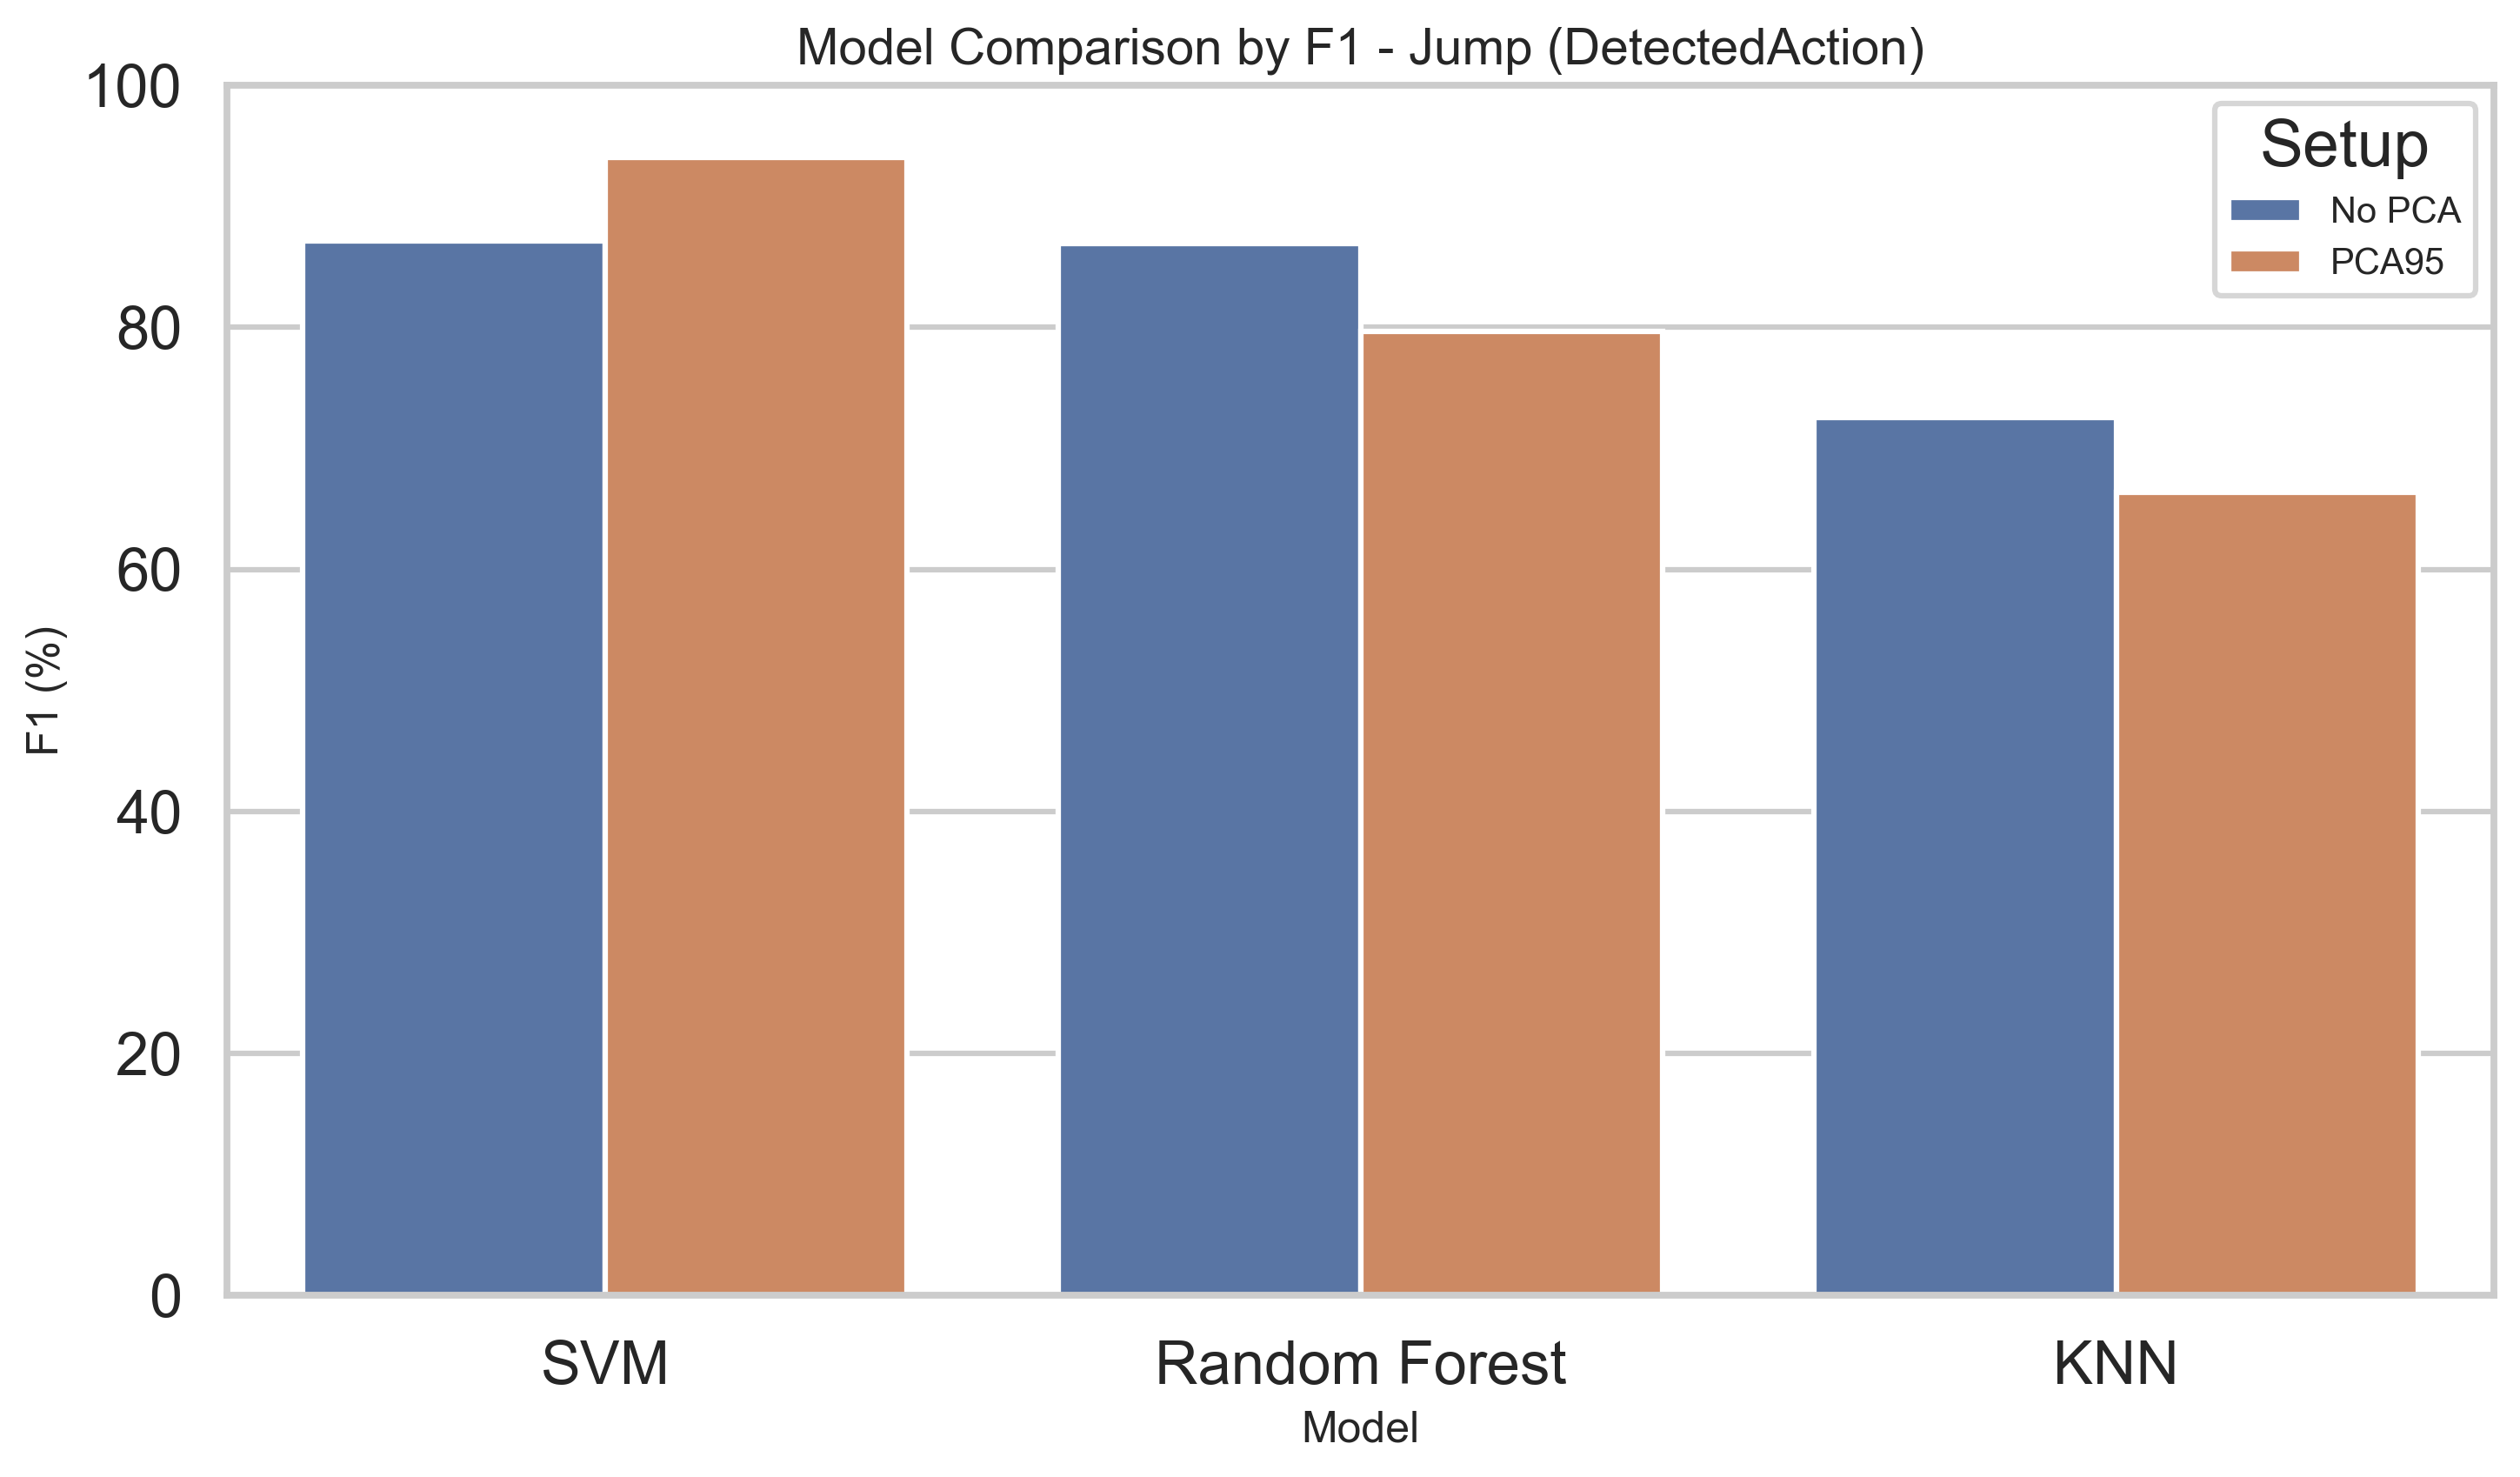
\includegraphics[width=0.85\linewidth]{Images/Generated/TaskResults/Jump/DetectedAction/model_comparison_f1.png}
    \caption{مقایسه عملکرد مدل‌ها بر اساس معیار \lr{F1} در فعالیت پریدن.}
    \label{fig:jump_detectedaction_model_comparison_f1}
\end{figure}

\noindent\textbf{توضیح شکل:} این نمودار اثر استفاده یا عدم استفاده از کاهش بعد را برای هر مدل نشان می‌دهد.
\vspace{0.8em}

\begin{figure}[H]
    \centering
    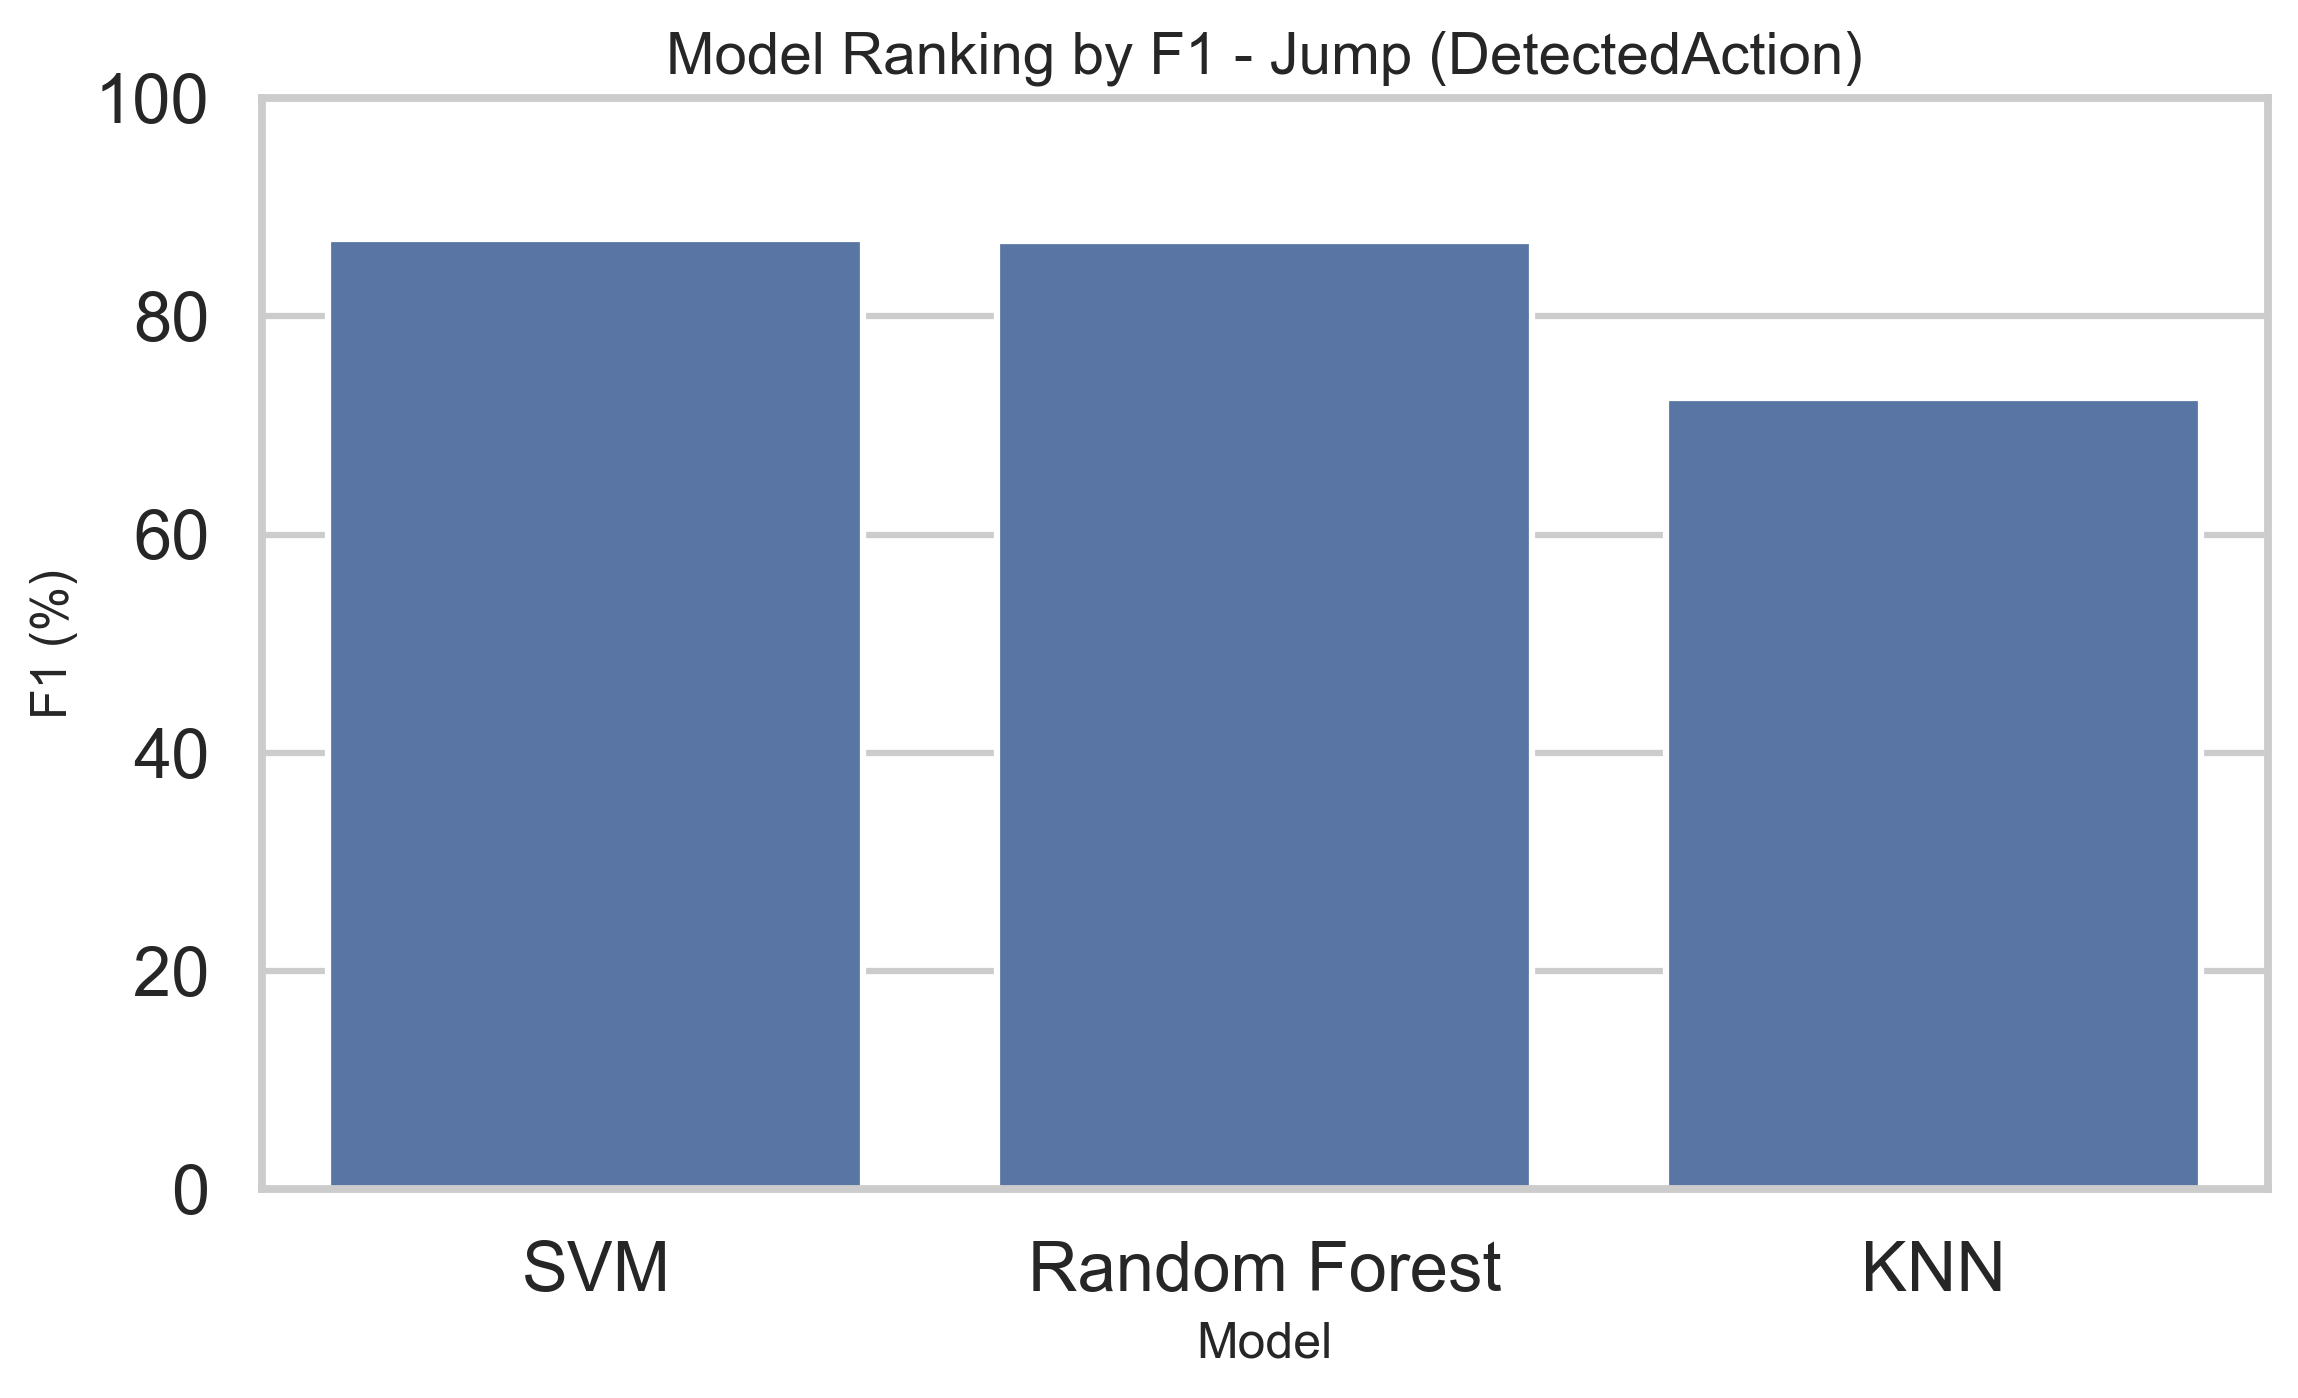
\includegraphics[width=0.85\linewidth]{Images/Generated/TaskResults/Jump/DetectedAction/model_ranking_f1.png}
    \caption{رتبه‌بندی مدل‌ها بر اساس معیار \lr{F1} در فعالیت پریدن.}
    \label{fig:jump_detectedaction_model_ranking_f1}
\end{figure}

\noindent\textbf{توضیح شکل:} این شکل جمع‌بندی سریعی از برتری نسبی مدل‌ها ارائه می‌دهد.
\vspace{0.8em}

\begin{figure}[H]
    \centering
    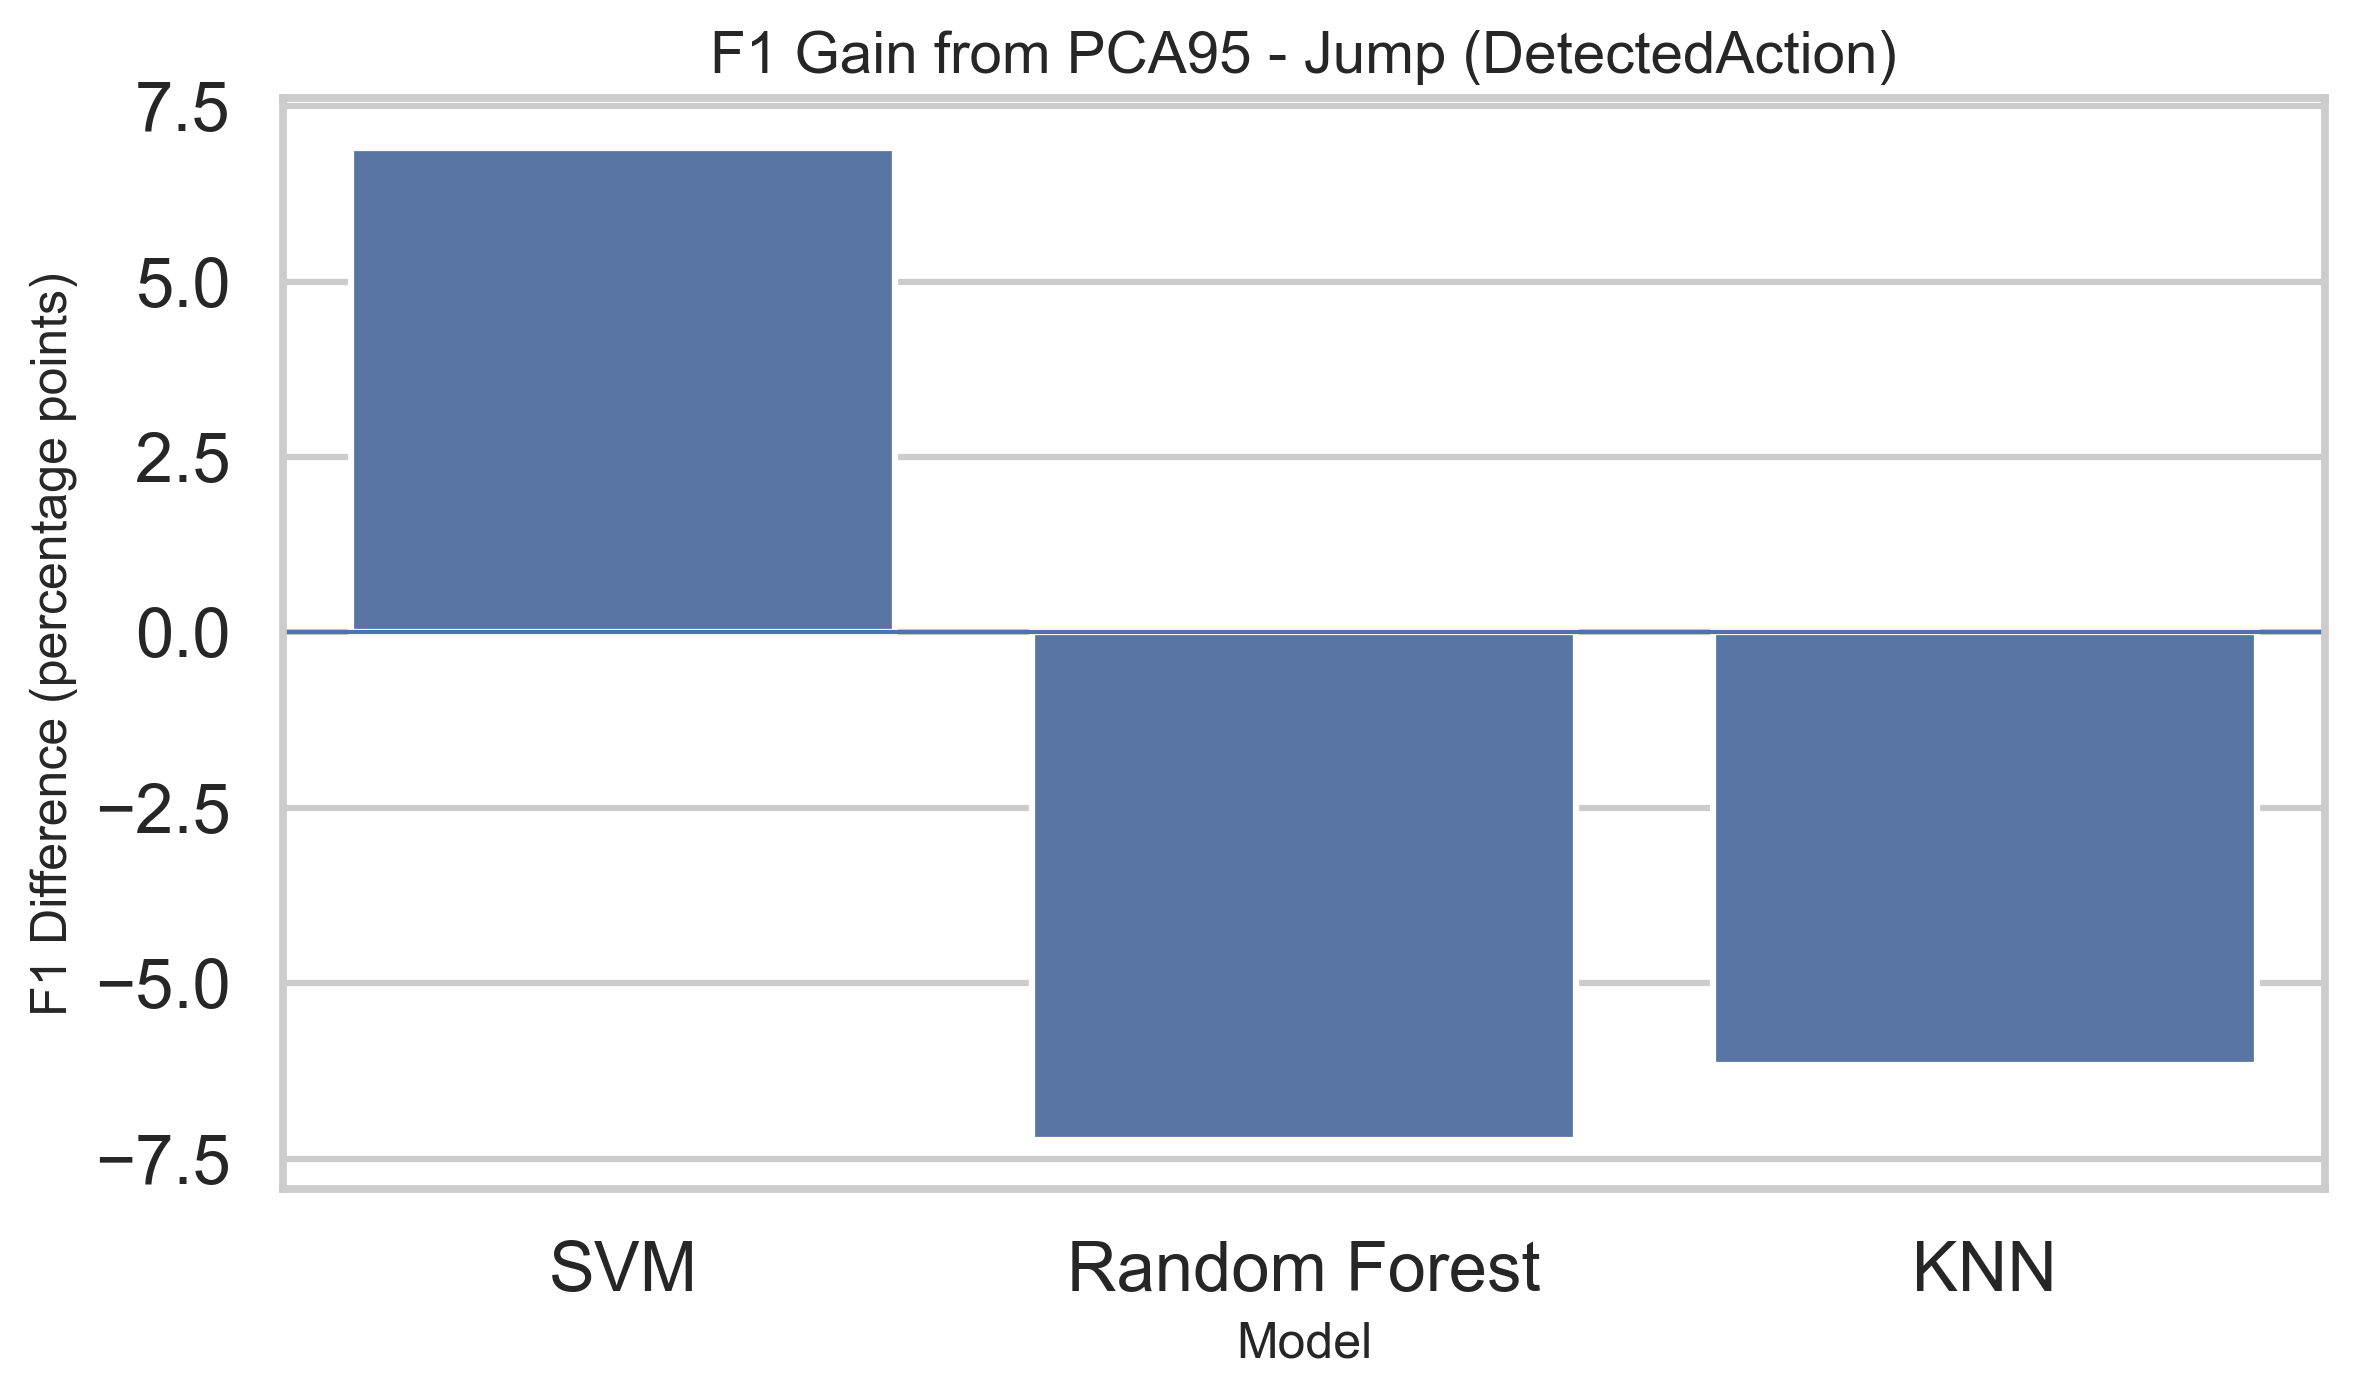
\includegraphics[width=0.85\linewidth]{Images/Generated/TaskResults/Jump/DetectedAction/f1_gain_pca_vs_no_pca.png}
    \caption{تغییر معیار \lr{F1} پس از اعمال \lr{PCA95} در فعالیت پریدن.}
    \label{fig:jump_detectedaction_f1_gain_pca}
\end{figure}

\noindent\textbf{توضیح شکل:} این شکل نشان می‌دهد کاهش بعد برای هر مدل سودمند بوده یا موجب افت عملکرد شده است.
\vspace{0.8em}

\begin{figure}[H]
    \centering
    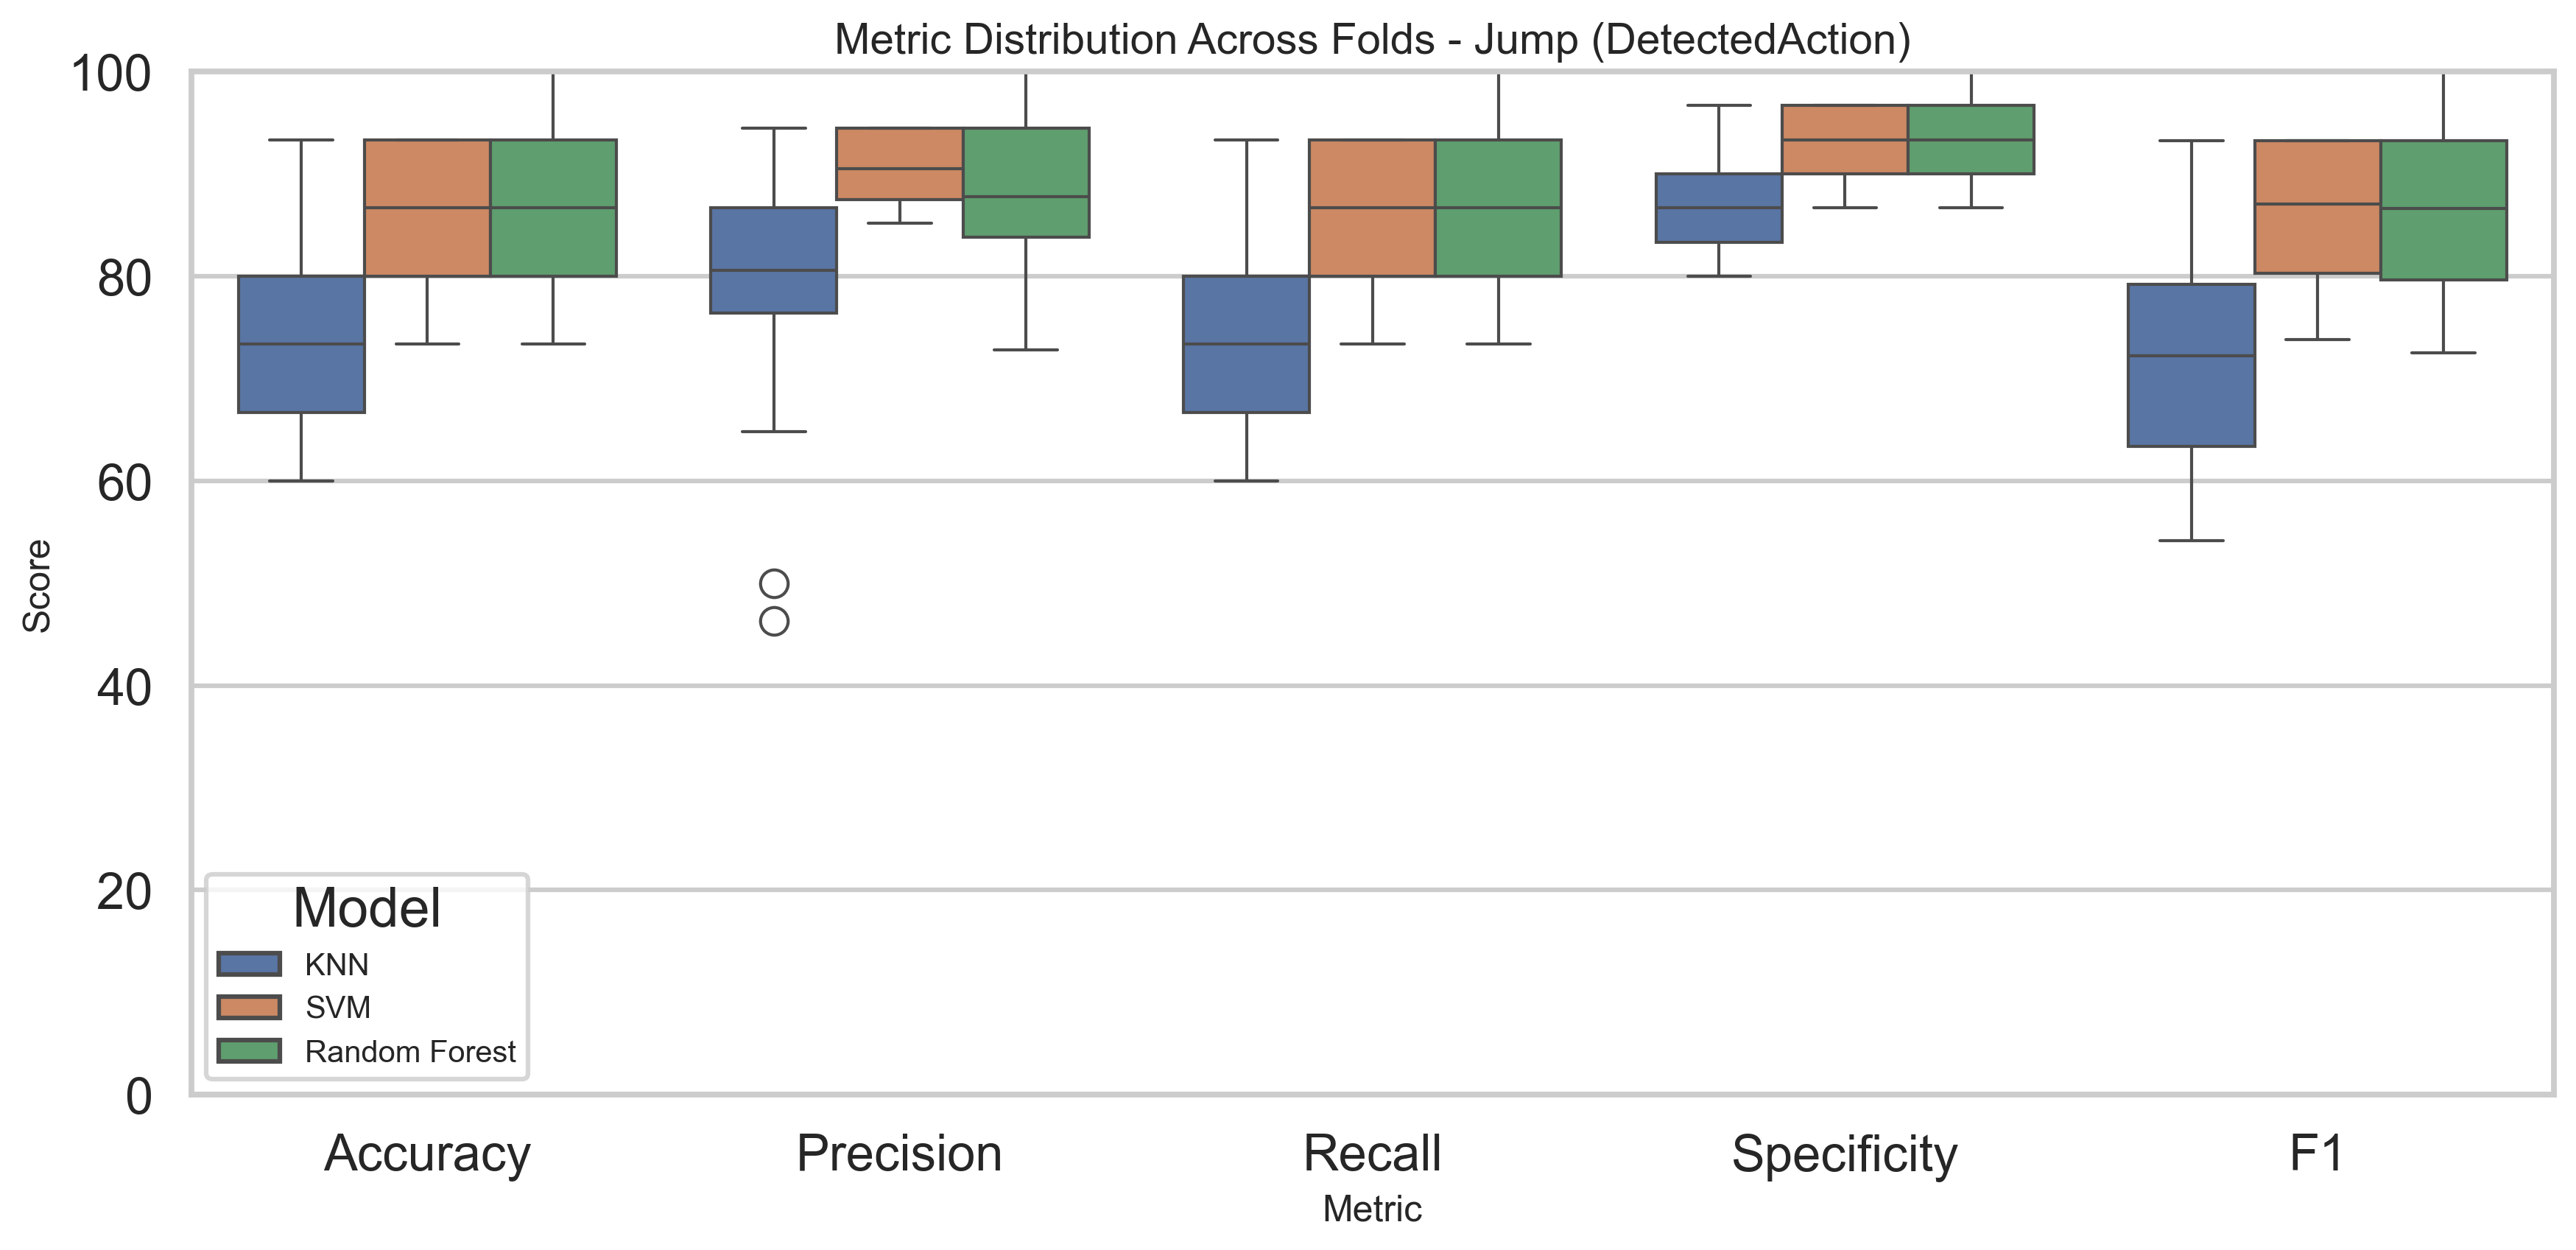
\includegraphics[width=0.85\linewidth]{Images/Generated/TaskResults/Jump/DetectedAction/metric_boxplots.png}
    \caption{پراکندگی معیارهای ارزیابی در تکرارهای اعتبارسنجی برای فعالیت پریدن.}
    \label{fig:jump_detectedaction_metric_boxplots}
\end{figure}

\noindent\textbf{توضیح شکل:} این شکل پایداری مدل‌ها را در foldهای مختلف نشان می‌دهد.
\vspace{0.8em}

\begin{figure}[H]
    \centering
    
\includegraphics[width=0.85\linewidth]{Images/Generated/TaskResults/Jump/DetectedAction/confusion_matrices_no_pca.png}
    \caption{ماتریس درهم‌ریختگی نرمال‌شده مدل‌ها در فعالیت پریدن (no_pca).}
    \label{fig:jump_detectedaction_confusion_no_pca}
\end{figure}

\noindent\textbf{توضیح شکل:} این شکل مشخص می‌کند خطاهای اصلی بین کدام کلاس‌های عملکردی رخ داده است.
\vspace{0.8em}

\begin{figure}[H]
    \centering
    
\includegraphics[width=0.85\linewidth]{Images/Generated/TaskResults/Jump/DetectedAction/per_class_recall_no_pca.png}
    \caption{مقایسه \lr{Recall} هر کلاس در فعالیت پریدن (no_pca).}
    \label{fig:jump_detectedaction_per_class_recall_no_pca}
\end{figure}

\noindent\textbf{توضیح شکل:} این نمودار حساسیت مدل‌ها نسبت به هر سطح عملکردی را نشان می‌دهد.
\vspace{0.8em}

\begin{figure}[H]
    \centering
    
\includegraphics[width=0.85\linewidth]{Images/Generated/TaskResults/Jump/DetectedAction/confusion_matrices_pca95.png}
    \caption{ماتریس درهم‌ریختگی نرمال‌شده مدل‌ها در فعالیت پریدن (pca95).}
    \label{fig:jump_detectedaction_confusion_pca95}
\end{figure}

\noindent\textbf{توضیح شکل:} این شکل مشخص می‌کند خطاهای اصلی بین کدام کلاس‌های عملکردی رخ داده است.
\vspace{0.8em}

\begin{figure}[H]
    \centering
    
\includegraphics[width=0.85\linewidth]{Images/Generated/TaskResults/Jump/DetectedAction/per_class_recall_pca95.png}
    \caption{مقایسه \lr{Recall} هر کلاس در فعالیت پریدن (pca95).}
    \label{fig:jump_detectedaction_per_class_recall_pca95}
\end{figure}

\noindent\textbf{توضیح شکل:} این نمودار حساسیت مدل‌ها نسبت به هر سطح عملکردی را نشان می‌دهد.
\vspace{0.8em}

\begin{figure}[H]
    \centering
    
\includegraphics[width=0.85\linewidth]{Images/Generated/TaskResults/Jump/DetectedAction/rf_top_feature_importance.png}
    \caption{20 ویژگی برتر بر اساس اهمیت در مدل \lr{Random Forest} برای فعالیت پریدن.}
    \label{fig:jump_detectedaction_rf_importance}
\end{figure}

\noindent\textbf{توضیح شکل:} این شکل نشان می‌دهد کدام حسگرها، محورها و شاخص‌های آماری نقش بیشتری در تصمیم‌گیری مدل داشته‌اند.
\vspace{0.8em}

\begin{figure}[H]
    \centering
    
\includegraphics[width=0.85\linewidth]{Images/Generated/TaskResults/Jump/DetectedAction/class_centroid_feature_heatmap.png}
    \caption{میانگین نرمال‌شده ویژگی‌های برتر در کلاس‌های مختلف فعالیت پریدن.}
    \label{fig:jump_detectedaction_class_centroid_heatmap}
\end{figure}

\noindent\textbf{توضیح شکل:} این نقشه حرارتی الگوی میانگین ویژگی‌ها را در هر سطح عملکردی نمایش می‌دهد.
\vspace{0.8em}

\begin{figure}[H]
    \centering
    
\includegraphics[width=0.85\linewidth]{Images/Generated/TaskResults/Jump/DetectedAction/svm_metrics_vs_pca_components.png}
    \caption{تغییر عملکرد مدل \lr{SVM} نسبت به تعداد مؤلفه‌های اصلی در فعالیت پریدن.}
    \label{fig:jump_detectedaction_svm_metrics_vs_pca_components}
\end{figure}

\noindent\textbf{توضیح شکل:} این نمودار برای انتخاب بازه مناسب تعداد مؤلفه‌های اصلی استفاده می‌شود.
\vspace{0.8em}

\begin{figure}[H]
    \centering
    
\includegraphics[width=0.85\linewidth]{Images/Generated/TaskResults/Jump/DetectedAction/models_f1_vs_pca_components.png}
    \caption{مقایسه مدل‌ها نسبت به تعداد مؤلفه‌های اصلی در فعالیت پریدن.}
    \label{fig:jump_detectedaction_models_f1_vs_pca_components}
\end{figure}

\noindent\textbf{توضیح شکل:} این نمودار نشان می‌دهد انتخاب تعداد مؤلفه‌ها و انتخاب مدل باید هم‌زمان انجام شود.
\vspace{0.8em}


\subsection*{نمودارهای فعالیت ایستادن}

\subsubsection*{داده‌های اصلی}

\begin{figure}[H]
    \centering
    
\includegraphics[width=0.85\linewidth]{Images/Generated/TaskResults/Stand/Normal/signal_sample.png}
    \caption{نمونه سیگنال‌های ثبت‌شده در فعالیت ایستادن (داده‌های اصلی).}
    \label{fig:stand_normal_signal_sample}
\end{figure}

\noindent\textbf{توضیح شکل:} این شکل نمایی از ماهیت زمانی سیگنال‌های حسگرها را برای فعالیت مورد نظر نشان می‌دهد.
\vspace{0.8em}

\begin{figure}[H]
    \centering
    
\includegraphics[width=0.85\linewidth]{Images/Generated/TaskResults/Stand/Normal/class_distribution.png}
    \caption{توزیع تعداد نمونه‌ها در سطوح عملکردی فعالیت ایستادن.}
    \label{fig:stand_normal_class_distribution}
\end{figure}

\noindent\textbf{توضیح شکل:} این نمودار برای بررسی تعادل داده‌ها بین کلاس‌های صفر، یک و دو استفاده می‌شود.
\vspace{0.8em}

\begin{figure}[H]
    \centering
    
\includegraphics[width=0.85\linewidth]{Images/Generated/TaskResults/Stand/Normal/feature_correlation_heatmap.png}
    \caption{نقشه همبستگی 20 ویژگی با بیشترین واریانس در فعالیت ایستادن.}
    \label{fig:stand_normal_feature_correlation}
\end{figure}

\noindent\textbf{توضیح شکل:} این نمودار وجود اطلاعات تکراری در فضای ویژگی را نشان می‌دهد و استفاده از کاهش بعد را توجیه می‌کند.
\vspace{0.8em}

\begin{figure}[H]
    \centering
    
\includegraphics[width=0.85\linewidth]{Images/Generated/TaskResults/Stand/Normal/pca_variance_curve.png}
    \caption{درصد واریانس توضیح‌داده‌شده و واریانس تجمعی مؤلفه‌های اصلی در فعالیت ایستادن.}
    \label{fig:stand_normal_pca_variance}
\end{figure}

\noindent\textbf{توضیح شکل:} این شکل مبنای انتخاب آستانه ۹۵ درصد و تعیین تعداد مؤلفه‌های نگه‌داشته‌شده را نشان می‌دهد.
\vspace{0.8em}

\begin{figure}[H]
    \centering
    
\includegraphics[width=0.85\linewidth]{Images/Generated/TaskResults/Stand/Normal/pca_scatter_pc1_pc2.png}
    \caption{پراکندگی نمونه‌های فعالیت ایستادن در فضای دو مؤلفه اصلی اول.}
    \label{fig:stand_normal_pca_scatter}
\end{figure}

\noindent\textbf{توضیح شکل:} این شکل یک تصویر اولیه از جدایی یا هم‌پوشانی کلاس‌ها در فضای کاهش‌یافته ارائه می‌دهد.
\vspace{0.8em}

\begin{figure}[H]
    \centering
    
\includegraphics[width=0.85\linewidth]{Images/Generated/TaskResults/Stand/Normal/model_comparison_f1.png}
    \caption{مقایسه عملکرد مدل‌ها بر اساس معیار \lr{F1} در فعالیت ایستادن.}
    \label{fig:stand_normal_model_comparison_f1}
\end{figure}

\noindent\textbf{توضیح شکل:} این نمودار اثر استفاده یا عدم استفاده از کاهش بعد را برای هر مدل نشان می‌دهد.
\vspace{0.8em}

\begin{figure}[H]
    \centering
    
\includegraphics[width=0.85\linewidth]{Images/Generated/TaskResults/Stand/Normal/model_ranking_f1.png}
    \caption{رتبه‌بندی مدل‌ها بر اساس معیار \lr{F1} در فعالیت ایستادن.}
    \label{fig:stand_normal_model_ranking_f1}
\end{figure}

\noindent\textbf{توضیح شکل:} این شکل جمع‌بندی سریعی از برتری نسبی مدل‌ها ارائه می‌دهد.
\vspace{0.8em}

\begin{figure}[H]
    \centering
    
\includegraphics[width=0.85\linewidth]{Images/Generated/TaskResults/Stand/Normal/f1_gain_pca_vs_no_pca.png}
    \caption{تغییر معیار \lr{F1} پس از اعمال \lr{PCA95} در فعالیت ایستادن.}
    \label{fig:stand_normal_f1_gain_pca}
\end{figure}

\noindent\textbf{توضیح شکل:} این شکل نشان می‌دهد کاهش بعد برای هر مدل سودمند بوده یا موجب افت عملکرد شده است.
\vspace{0.8em}

\begin{figure}[H]
    \centering
    
\includegraphics[width=0.85\linewidth]{Images/Generated/TaskResults/Stand/Normal/metric_boxplots.png}
    \caption{پراکندگی معیارهای ارزیابی در تکرارهای اعتبارسنجی برای فعالیت ایستادن.}
    \label{fig:stand_normal_metric_boxplots}
\end{figure}

\noindent\textbf{توضیح شکل:} این شکل پایداری مدل‌ها را در foldهای مختلف نشان می‌دهد.
\vspace{0.8em}

\begin{figure}[H]
    \centering
    
\includegraphics[width=0.85\linewidth]{Images/Generated/TaskResults/Stand/Normal/confusion_matrices_no_pca.png}
    \caption{ماتریس درهم‌ریختگی نرمال‌شده مدل‌ها در فعالیت ایستادن (no_pca).}
    \label{fig:stand_normal_confusion_no_pca}
\end{figure}

\noindent\textbf{توضیح شکل:} این شکل مشخص می‌کند خطاهای اصلی بین کدام کلاس‌های عملکردی رخ داده است.
\vspace{0.8em}

\begin{figure}[H]
    \centering
    
\includegraphics[width=0.85\linewidth]{Images/Generated/TaskResults/Stand/Normal/per_class_recall_no_pca.png}
    \caption{مقایسه \lr{Recall} هر کلاس در فعالیت ایستادن (no_pca).}
    \label{fig:stand_normal_per_class_recall_no_pca}
\end{figure}

\noindent\textbf{توضیح شکل:} این نمودار حساسیت مدل‌ها نسبت به هر سطح عملکردی را نشان می‌دهد.
\vspace{0.8em}

\begin{figure}[H]
    \centering
    
\includegraphics[width=0.85\linewidth]{Images/Generated/TaskResults/Stand/Normal/confusion_matrices_pca95.png}
    \caption{ماتریس درهم‌ریختگی نرمال‌شده مدل‌ها در فعالیت ایستادن (pca95).}
    \label{fig:stand_normal_confusion_pca95}
\end{figure}

\noindent\textbf{توضیح شکل:} این شکل مشخص می‌کند خطاهای اصلی بین کدام کلاس‌های عملکردی رخ داده است.
\vspace{0.8em}

\begin{figure}[H]
    \centering
    
\includegraphics[width=0.85\linewidth]{Images/Generated/TaskResults/Stand/Normal/per_class_recall_pca95.png}
    \caption{مقایسه \lr{Recall} هر کلاس در فعالیت ایستادن (pca95).}
    \label{fig:stand_normal_per_class_recall_pca95}
\end{figure}

\noindent\textbf{توضیح شکل:} این نمودار حساسیت مدل‌ها نسبت به هر سطح عملکردی را نشان می‌دهد.
\vspace{0.8em}

\begin{figure}[H]
    \centering
    
\includegraphics[width=0.85\linewidth]{Images/Generated/TaskResults/Stand/Normal/rf_top_feature_importance.png}
    \caption{20 ویژگی برتر بر اساس اهمیت در مدل \lr{Random Forest} برای فعالیت ایستادن.}
    \label{fig:stand_normal_rf_importance}
\end{figure}

\noindent\textbf{توضیح شکل:} این شکل نشان می‌دهد کدام حسگرها، محورها و شاخص‌های آماری نقش بیشتری در تصمیم‌گیری مدل داشته‌اند.
\vspace{0.8em}

\begin{figure}[H]
    \centering
    
\includegraphics[width=0.85\linewidth]{Images/Generated/TaskResults/Stand/Normal/class_centroid_feature_heatmap.png}
    \caption{میانگین نرمال‌شده ویژگی‌های برتر در کلاس‌های مختلف فعالیت ایستادن.}
    \label{fig:stand_normal_class_centroid_heatmap}
\end{figure}

\noindent\textbf{توضیح شکل:} این نقشه حرارتی الگوی میانگین ویژگی‌ها را در هر سطح عملکردی نمایش می‌دهد.
\vspace{0.8em}

\begin{figure}[H]
    \centering
    
\includegraphics[width=0.85\linewidth]{Images/Generated/TaskResults/Stand/Normal/svm_metrics_vs_pca_components.png}
    \caption{تغییر عملکرد مدل \lr{SVM} نسبت به تعداد مؤلفه‌های اصلی در فعالیت ایستادن.}
    \label{fig:stand_normal_svm_metrics_vs_pca_components}
\end{figure}

\noindent\textbf{توضیح شکل:} این نمودار برای انتخاب بازه مناسب تعداد مؤلفه‌های اصلی استفاده می‌شود.
\vspace{0.8em}

\begin{figure}[H]
    \centering
    
\includegraphics[width=0.85\linewidth]{Images/Generated/TaskResults/Stand/Normal/models_f1_vs_pca_components.png}
    \caption{مقایسه مدل‌ها نسبت به تعداد مؤلفه‌های اصلی در فعالیت ایستادن.}
    \label{fig:stand_normal_models_f1_vs_pca_components}
\end{figure}

\noindent\textbf{توضیح شکل:} این نمودار نشان می‌دهد انتخاب تعداد مؤلفه‌ها و انتخاب مدل باید هم‌زمان انجام شود.
\vspace{0.8em}

\subsection*{نمودارهای فعالیت بلند شدن از صندلی}

\subsubsection*{داده‌های اصلی}

\begin{figure}[H]
    \centering
    
\includegraphics[width=0.85\linewidth]{Images/Generated/TaskResults/Sit_To_Stand/Normal/signal_sample.png}
    \caption{نمونه سیگنال‌های ثبت‌شده در فعالیت بلند شدن از صندلی (داده‌های اصلی).}
    \label{fig:sit_to_stand_normal_signal_sample}
\end{figure}

\noindent\textbf{توضیح شکل:} این شکل نمایی از ماهیت زمانی سیگنال‌های حسگرها را برای فعالیت مورد نظر نشان می‌دهد.
\vspace{0.8em}

\begin{figure}[H]
    \centering
    
\includegraphics[width=0.85\linewidth]{Images/Generated/TaskResults/Sit_To_Stand/Normal/class_distribution.png}
    \caption{توزیع تعداد نمونه‌ها در سطوح عملکردی فعالیت بلند شدن از صندلی.}
    \label{fig:sit_to_stand_normal_class_distribution}
\end{figure}

\noindent\textbf{توضیح شکل:} این نمودار برای بررسی تعادل داده‌ها بین کلاس‌های صفر، یک و دو استفاده می‌شود.
\vspace{0.8em}

\begin{figure}[H]
    \centering
    
\includegraphics[width=0.85\linewidth]{Images/Generated/TaskResults/Sit_To_Stand/Normal/feature_correlation_heatmap.png}
    \caption{نقشه همبستگی 20 ویژگی با بیشترین واریانس در فعالیت بلند شدن از صندلی.}
    \label{fig:sit_to_stand_normal_feature_correlation}
\end{figure}

\noindent\textbf{توضیح شکل:} این نمودار وجود اطلاعات تکراری در فضای ویژگی را نشان می‌دهد و استفاده از کاهش بعد را توجیه می‌کند.
\vspace{0.8em}

\begin{figure}[H]
    \centering
    
\includegraphics[width=0.85\linewidth]{Images/Generated/TaskResults/Sit_To_Stand/Normal/pca_variance_curve.png}
    \caption{درصد واریانس توضیح‌داده‌شده و واریانس تجمعی مؤلفه‌های اصلی در فعالیت بلند شدن از صندلی.}
    \label{fig:sit_to_stand_normal_pca_variance}
\end{figure}

\noindent\textbf{توضیح شکل:} این شکل مبنای انتخاب آستانه ۹۵ درصد و تعیین تعداد مؤلفه‌های نگه‌داشته‌شده را نشان می‌دهد.
\vspace{0.8em}

\begin{figure}[H]
    \centering
    
\includegraphics[width=0.85\linewidth]{Images/Generated/TaskResults/Sit_To_Stand/Normal/pca_scatter_pc1_pc2.png}
    \caption{پراکندگی نمونه‌های فعالیت بلند شدن از صندلی در فضای دو مؤلفه اصلی اول.}
    \label{fig:sit_to_stand_normal_pca_scatter}
\end{figure}

\noindent\textbf{توضیح شکل:} این شکل یک تصویر اولیه از جدایی یا هم‌پوشانی کلاس‌ها در فضای کاهش‌یافته ارائه می‌دهد.
\vspace{0.8em}

\begin{figure}[H]
    \centering
    
\includegraphics[width=0.85\linewidth]{Images/Generated/TaskResults/Sit_To_Stand/Normal/model_comparison_f1.png}
    \caption{مقایسه عملکرد مدل‌ها بر اساس معیار \lr{F1} در فعالیت بلند شدن از صندلی.}
    \label{fig:sit_to_stand_normal_model_comparison_f1}
\end{figure}

\noindent\textbf{توضیح شکل:} این نمودار اثر استفاده یا عدم استفاده از کاهش بعد را برای هر مدل نشان می‌دهد.
\vspace{0.8em}

\begin{figure}[H]
    \centering
    
\includegraphics[width=0.85\linewidth]{Images/Generated/TaskResults/Sit_To_Stand/Normal/model_ranking_f1.png}
    \caption{رتبه‌بندی مدل‌ها بر اساس معیار \lr{F1} در فعالیت بلند شدن از صندلی.}
    \label{fig:sit_to_stand_normal_model_ranking_f1}
\end{figure}

\noindent\textbf{توضیح شکل:} این شکل جمع‌بندی سریعی از برتری نسبی مدل‌ها ارائه می‌دهد.
\vspace{0.8em}

\begin{figure}[H]
    \centering
    
\includegraphics[width=0.85\linewidth]{Images/Generated/TaskResults/Sit_To_Stand/Normal/f1_gain_pca_vs_no_pca.png}
    \caption{تغییر معیار \lr{F1} پس از اعمال \lr{PCA95} در فعالیت بلند شدن از صندلی.}
    \label{fig:sit_to_stand_normal_f1_gain_pca}
\end{figure}

\noindent\textbf{توضیح شکل:} این شکل نشان می‌دهد کاهش بعد برای هر مدل سودمند بوده یا موجب افت عملکرد شده است.
\vspace{0.8em}

\begin{figure}[H]
    \centering
    
\includegraphics[width=0.85\linewidth]{Images/Generated/TaskResults/Sit_To_Stand/Normal/metric_boxplots.png}
    \caption{پراکندگی معیارهای ارزیابی در تکرارهای اعتبارسنجی برای فعالیت بلند شدن از صندلی.}
    \label{fig:sit_to_stand_normal_metric_boxplots}
\end{figure}

\noindent\textbf{توضیح شکل:} این شکل پایداری مدل‌ها را در foldهای مختلف نشان می‌دهد.
\vspace{0.8em}

\begin{figure}[H]
    \centering
    
\includegraphics[width=0.85\linewidth]{Images/Generated/TaskResults/Sit_To_Stand/Normal/confusion_matrices_no_pca.png}
    \caption{ماتریس درهم‌ریختگی نرمال‌شده مدل‌ها در فعالیت بلند شدن از صندلی (no_pca).}
    \label{fig:sit_to_stand_normal_confusion_no_pca}
\end{figure}

\noindent\textbf{توضیح شکل:} این شکل مشخص می‌کند خطاهای اصلی بین کدام کلاس‌های عملکردی رخ داده است.
\vspace{0.8em}

\begin{figure}[H]
    \centering
    
\includegraphics[width=0.85\linewidth]{Images/Generated/TaskResults/Sit_To_Stand/Normal/per_class_recall_no_pca.png}
    \caption{مقایسه \lr{Recall} هر کلاس در فعالیت بلند شدن از صندلی (no_pca).}
    \label{fig:sit_to_stand_normal_per_class_recall_no_pca}
\end{figure}

\noindent\textbf{توضیح شکل:} این نمودار حساسیت مدل‌ها نسبت به هر سطح عملکردی را نشان می‌دهد.
\vspace{0.8em}

\begin{figure}[H]
    \centering
    
\includegraphics[width=0.85\linewidth]{Images/Generated/TaskResults/Sit_To_Stand/Normal/confusion_matrices_pca95.png}
    \caption{ماتریس درهم‌ریختگی نرمال‌شده مدل‌ها در فعالیت بلند شدن از صندلی (pca95).}
    \label{fig:sit_to_stand_normal_confusion_pca95}
\end{figure}

\noindent\textbf{توضیح شکل:} این شکل مشخص می‌کند خطاهای اصلی بین کدام کلاس‌های عملکردی رخ داده است.
\vspace{0.8em}

\begin{figure}[H]
    \centering
    
\includegraphics[width=0.85\linewidth]{Images/Generated/TaskResults/Sit_To_Stand/Normal/per_class_recall_pca95.png}
    \caption{مقایسه \lr{Recall} هر کلاس در فعالیت بلند شدن از صندلی (pca95).}
    \label{fig:sit_to_stand_normal_per_class_recall_pca95}
\end{figure}

\noindent\textbf{توضیح شکل:} این نمودار حساسیت مدل‌ها نسبت به هر سطح عملکردی را نشان می‌دهد.
\vspace{0.8em}

\begin{figure}[H]
    \centering
    
\includegraphics[width=0.85\linewidth]{Images/Generated/TaskResults/Sit_To_Stand/Normal/rf_top_feature_importance.png}
    \caption{20 ویژگی برتر بر اساس اهمیت در مدل \lr{Random Forest} برای فعالیت بلند شدن از صندلی.}
    \label{fig:sit_to_stand_normal_rf_importance}
\end{figure}

\noindent\textbf{توضیح شکل:} این شکل نشان می‌دهد کدام حسگرها، محورها و شاخص‌های آماری نقش بیشتری در تصمیم‌گیری مدل داشته‌اند.
\vspace{0.8em}

\begin{figure}[H]
    \centering
    
\includegraphics[width=0.85\linewidth]{Images/Generated/TaskResults/Sit_To_Stand/Normal/class_centroid_feature_heatmap.png}
    \caption{میانگین نرمال‌شده ویژگی‌های برتر در کلاس‌های مختلف فعالیت بلند شدن از صندلی.}
    \label{fig:sit_to_stand_normal_class_centroid_heatmap}
\end{figure}

\noindent\textbf{توضیح شکل:} این نقشه حرارتی الگوی میانگین ویژگی‌ها را در هر سطح عملکردی نمایش می‌دهد.
\vspace{0.8em}

\begin{figure}[H]
    \centering
    
\includegraphics[width=0.85\linewidth]{Images/Generated/TaskResults/Sit_To_Stand/Normal/svm_metrics_vs_pca_components.png}
    \caption{تغییر عملکرد مدل \lr{SVM} نسبت به تعداد مؤلفه‌های اصلی در فعالیت بلند شدن از صندلی.}
    \label{fig:sit_to_stand_normal_svm_metrics_vs_pca_components}
\end{figure}

\noindent\textbf{توضیح شکل:} این نمودار برای انتخاب بازه مناسب تعداد مؤلفه‌های اصلی استفاده می‌شود.
\vspace{0.8em}

\begin{figure}[H]
    \centering
    
\includegraphics[width=0.85\linewidth]{Images/Generated/TaskResults/Sit_To_Stand/Normal/models_f1_vs_pca_components.png}
    \caption{مقایسه مدل‌ها نسبت به تعداد مؤلفه‌های اصلی در فعالیت بلند شدن از صندلی.}
    \label{fig:sit_to_stand_normal_models_f1_vs_pca_components}
\end{figure}

\noindent\textbf{توضیح شکل:} این نمودار نشان می‌دهد انتخاب تعداد مؤلفه‌ها و انتخاب مدل باید هم‌زمان انجام شود.
\vspace{0.8em}

\subsubsection*{داده‌های جداسازی‌شده با تشخیص فعالیت}

\begin{figure}[H]
    \centering
    
\includegraphics[width=0.85\linewidth]{Images/Generated/TaskResults/Sit_To_Stand/DetectedAction/signal_sample.png}
    \caption{نمونه سیگنال‌های ثبت‌شده در فعالیت بلند شدن از صندلی (داده‌های جداسازی‌شده با تشخیص فعالیت).}
    \label{fig:sit_to_stand_detectedaction_signal_sample}
\end{figure}

\noindent\textbf{توضیح شکل:} این شکل نمایی از ماهیت زمانی سیگنال‌های حسگرها را برای فعالیت مورد نظر نشان می‌دهد.
\vspace{0.8em}

\begin{figure}[H]
    \centering
    
\includegraphics[width=0.85\linewidth]{Images/Generated/TaskResults/Sit_To_Stand/DetectedAction/class_distribution.png}
    \caption{توزیع تعداد نمونه‌ها در سطوح عملکردی فعالیت بلند شدن از صندلی.}
    \label{fig:sit_to_stand_detectedaction_class_distribution}
\end{figure}

\noindent\textbf{توضیح شکل:} این نمودار برای بررسی تعادل داده‌ها بین کلاس‌های صفر، یک و دو استفاده می‌شود.
\vspace{0.8em}

\begin{figure}[H]
    \centering
    
\includegraphics[width=0.85\linewidth]{Images/Generated/TaskResults/Sit_To_Stand/DetectedAction/feature_correlation_heatmap.png}
    \caption{نقشه همبستگی 20 ویژگی با بیشترین واریانس در فعالیت بلند شدن از صندلی.}
    \label{fig:sit_to_stand_detectedaction_feature_correlation}
\end{figure}

\noindent\textbf{توضیح شکل:} این نمودار وجود اطلاعات تکراری در فضای ویژگی را نشان می‌دهد و استفاده از کاهش بعد را توجیه می‌کند.
\vspace{0.8em}

\begin{figure}[H]
    \centering
    
\includegraphics[width=0.85\linewidth]{Images/Generated/TaskResults/Sit_To_Stand/DetectedAction/pca_variance_curve.png}
    \caption{درصد واریانس توضیح‌داده‌شده و واریانس تجمعی مؤلفه‌های اصلی در فعالیت بلند شدن از صندلی.}
    \label{fig:sit_to_stand_detectedaction_pca_variance}
\end{figure}

\noindent\textbf{توضیح شکل:} این شکل مبنای انتخاب آستانه ۹۵ درصد و تعیین تعداد مؤلفه‌های نگه‌داشته‌شده را نشان می‌دهد.
\vspace{0.8em}

\begin{figure}[H]
    \centering
    
\includegraphics[width=0.85\linewidth]{Images/Generated/TaskResults/Sit_To_Stand/DetectedAction/pca_scatter_pc1_pc2.png}
    \caption{پراکندگی نمونه‌های فعالیت بلند شدن از صندلی در فضای دو مؤلفه اصلی اول.}
    \label{fig:sit_to_stand_detectedaction_pca_scatter}
\end{figure}

\noindent\textbf{توضیح شکل:} این شکل یک تصویر اولیه از جدایی یا هم‌پوشانی کلاس‌ها در فضای کاهش‌یافته ارائه می‌دهد.
\vspace{0.8em}

\begin{figure}[H]
    \centering
    
\includegraphics[width=0.85\linewidth]{Images/Generated/TaskResults/Sit_To_Stand/DetectedAction/model_comparison_f1.png}
    \caption{مقایسه عملکرد مدل‌ها بر اساس معیار \lr{F1} در فعالیت بلند شدن از صندلی.}
    \label{fig:sit_to_stand_detectedaction_model_comparison_f1}
\end{figure}

\noindent\textbf{توضیح شکل:} این نمودار اثر استفاده یا عدم استفاده از کاهش بعد را برای هر مدل نشان می‌دهد.
\vspace{0.8em}

\begin{figure}[H]
    \centering
    
\includegraphics[width=0.85\linewidth]{Images/Generated/TaskResults/Sit_To_Stand/DetectedAction/model_ranking_f1.png}
    \caption{رتبه‌بندی مدل‌ها بر اساس معیار \lr{F1} در فعالیت بلند شدن از صندلی.}
    \label{fig:sit_to_stand_detectedaction_model_ranking_f1}
\end{figure}

\noindent\textbf{توضیح شکل:} این شکل جمع‌بندی سریعی از برتری نسبی مدل‌ها ارائه می‌دهد.
\vspace{0.8em}

\begin{figure}[H]
    \centering
    
\includegraphics[width=0.85\linewidth]{Images/Generated/TaskResults/Sit_To_Stand/DetectedAction/f1_gain_pca_vs_no_pca.png}
    \caption{تغییر معیار \lr{F1} پس از اعمال \lr{PCA95} در فعالیت بلند شدن از صندلی.}
    \label{fig:sit_to_stand_detectedaction_f1_gain_pca}
\end{figure}

\noindent\textbf{توضیح شکل:} این شکل نشان می‌دهد کاهش بعد برای هر مدل سودمند بوده یا موجب افت عملکرد شده است.
\vspace{0.8em}

\begin{figure}[H]
    \centering
    
\includegraphics[width=0.85\linewidth]{Images/Generated/TaskResults/Sit_To_Stand/DetectedAction/metric_boxplots.png}
    \caption{پراکندگی معیارهای ارزیابی در تکرارهای اعتبارسنجی برای فعالیت بلند شدن از صندلی.}
    \label{fig:sit_to_stand_detectedaction_metric_boxplots}
\end{figure}

\noindent\textbf{توضیح شکل:} این شکل پایداری مدل‌ها را در foldهای مختلف نشان می‌دهد.
\vspace{0.8em}

\begin{figure}[H]
    \centering
    
\includegraphics[width=0.85\linewidth]{Images/Generated/TaskResults/Sit_To_Stand/DetectedAction/confusion_matrices_no_pca.png}
    \caption{ماتریس درهم‌ریختگی نرمال‌شده مدل‌ها در فعالیت بلند شدن از صندلی (no_pca).}
    \label{fig:sit_to_stand_detectedaction_confusion_no_pca}
\end{figure}

\noindent\textbf{توضیح شکل:} این شکل مشخص می‌کند خطاهای اصلی بین کدام کلاس‌های عملکردی رخ داده است.
\vspace{0.8em}

\begin{figure}[H]
    \centering
    
\includegraphics[width=0.85\linewidth]{Images/Generated/TaskResults/Sit_To_Stand/DetectedAction/per_class_recall_no_pca.png}
    \caption{مقایسه \lr{Recall} هر کلاس در فعالیت بلند شدن از صندلی (no_pca).}
    \label{fig:sit_to_stand_detectedaction_per_class_recall_no_pca}
\end{figure}

\noindent\textbf{توضیح شکل:} این نمودار حساسیت مدل‌ها نسبت به هر سطح عملکردی را نشان می‌دهد.
\vspace{0.8em}

\begin{figure}[H]
    \centering
    
\includegraphics[width=0.85\linewidth]{Images/Generated/TaskResults/Sit_To_Stand/DetectedAction/confusion_matrices_pca95.png}
    \caption{ماتریس درهم‌ریختگی نرمال‌شده مدل‌ها در فعالیت بلند شدن از صندلی (pca95).}
    \label{fig:sit_to_stand_detectedaction_confusion_pca95}
\end{figure}

\noindent\textbf{توضیح شکل:} این شکل مشخص می‌کند خطاهای اصلی بین کدام کلاس‌های عملکردی رخ داده است.
\vspace{0.8em}

\begin{figure}[H]
    \centering
    
\includegraphics[width=0.85\linewidth]{Images/Generated/TaskResults/Sit_To_Stand/DetectedAction/per_class_recall_pca95.png}
    \caption{مقایسه \lr{Recall} هر کلاس در فعالیت بلند شدن از صندلی (pca95).}
    \label{fig:sit_to_stand_detectedaction_per_class_recall_pca95}
\end{figure}

\noindent\textbf{توضیح شکل:} این نمودار حساسیت مدل‌ها نسبت به هر سطح عملکردی را نشان می‌دهد.
\vspace{0.8em}

\begin{figure}[H]
    \centering
    
\includegraphics[width=0.85\linewidth]{Images/Generated/TaskResults/Sit_To_Stand/DetectedAction/rf_top_feature_importance.png}
    \caption{20 ویژگی برتر بر اساس اهمیت در مدل \lr{Random Forest} برای فعالیت بلند شدن از صندلی.}
    \label{fig:sit_to_stand_detectedaction_rf_importance}
\end{figure}

\noindent\textbf{توضیح شکل:} این شکل نشان می‌دهد کدام حسگرها، محورها و شاخص‌های آماری نقش بیشتری در تصمیم‌گیری مدل داشته‌اند.
\vspace{0.8em}

\begin{figure}[H]
    \centering
    
\includegraphics[width=0.85\linewidth]{Images/Generated/TaskResults/Sit_To_Stand/DetectedAction/class_centroid_feature_heatmap.png}
    \caption{میانگین نرمال‌شده ویژگی‌های برتر در کلاس‌های مختلف فعالیت بلند شدن از صندلی.}
    \label{fig:sit_to_stand_detectedaction_class_centroid_heatmap}
\end{figure}

\noindent\textbf{توضیح شکل:} این نقشه حرارتی الگوی میانگین ویژگی‌ها را در هر سطح عملکردی نمایش می‌دهد.
\vspace{0.8em}

\begin{figure}[H]
    \centering
    
\includegraphics[width=0.85\linewidth]{Images/Generated/TaskResults/Sit_To_Stand/DetectedAction/svm_metrics_vs_pca_components.png}
    \caption{تغییر عملکرد مدل \lr{SVM} نسبت به تعداد مؤلفه‌های اصلی در فعالیت بلند شدن از صندلی.}
    \label{fig:sit_to_stand_detectedaction_svm_metrics_vs_pca_components}
\end{figure}

\noindent\textbf{توضیح شکل:} این نمودار برای انتخاب بازه مناسب تعداد مؤلفه‌های اصلی استفاده می‌شود.
\vspace{0.8em}

\begin{figure}[H]
    \centering
    
\includegraphics[width=0.85\linewidth]{Images/Generated/TaskResults/Sit_To_Stand/DetectedAction/models_f1_vs_pca_components.png}
    \caption{مقایسه مدل‌ها نسبت به تعداد مؤلفه‌های اصلی در فعالیت بلند شدن از صندلی.}
    \label{fig:sit_to_stand_detectedaction_models_f1_vs_pca_components}
\end{figure}

\noindent\textbf{توضیح شکل:} این نمودار نشان می‌دهد انتخاب تعداد مؤلفه‌ها و انتخاب مدل باید هم‌زمان انجام شود.
\vspace{0.8em}

\subsection*{نمودارهای فعالیت پریدن}

\subsubsection*{داده‌های اصلی}

\begin{figure}[H]
    \centering
    
\includegraphics[width=0.85\linewidth]{Images/Generated/TaskResults/Jump/Normal/signal_sample.png}
    \caption{نمونه سیگنال‌های ثبت‌شده در فعالیت پریدن (داده‌های اصلی).}
    \label{fig:jump_normal_signal_sample}
\end{figure}

\noindent\textbf{توضیح شکل:} این شکل نمایی از ماهیت زمانی سیگنال‌های حسگرها را برای فعالیت مورد نظر نشان می‌دهد.
\vspace{0.8em}

\begin{figure}[H]
    \centering
    
\includegraphics[width=0.85\linewidth]{Images/Generated/TaskResults/Jump/Normal/class_distribution.png}
    \caption{توزیع تعداد نمونه‌ها در سطوح عملکردی فعالیت پریدن.}
    \label{fig:jump_normal_class_distribution}
\end{figure}

\noindent\textbf{توضیح شکل:} این نمودار برای بررسی تعادل داده‌ها بین کلاس‌های صفر، یک و دو استفاده می‌شود.
\vspace{0.8em}

\begin{figure}[H]
    \centering
    
\includegraphics[width=0.85\linewidth]{Images/Generated/TaskResults/Jump/Normal/feature_correlation_heatmap.png}
    \caption{نقشه همبستگی 20 ویژگی با بیشترین واریانس در فعالیت پریدن.}
    \label{fig:jump_normal_feature_correlation}
\end{figure}

\noindent\textbf{توضیح شکل:} این نمودار وجود اطلاعات تکراری در فضای ویژگی را نشان می‌دهد و استفاده از کاهش بعد را توجیه می‌کند.
\vspace{0.8em}

\begin{figure}[H]
    \centering
    
\includegraphics[width=0.85\linewidth]{Images/Generated/TaskResults/Jump/Normal/pca_variance_curve.png}
    \caption{درصد واریانس توضیح‌داده‌شده و واریانس تجمعی مؤلفه‌های اصلی در فعالیت پریدن.}
    \label{fig:jump_normal_pca_variance}
\end{figure}

\noindent\textbf{توضیح شکل:} این شکل مبنای انتخاب آستانه ۹۵ درصد و تعیین تعداد مؤلفه‌های نگه‌داشته‌شده را نشان می‌دهد.
\vspace{0.8em}

\begin{figure}[H]
    \centering
    
\includegraphics[width=0.85\linewidth]{Images/Generated/TaskResults/Jump/Normal/pca_scatter_pc1_pc2.png}
    \caption{پراکندگی نمونه‌های فعالیت پریدن در فضای دو مؤلفه اصلی اول.}
    \label{fig:jump_normal_pca_scatter}
\end{figure}

\noindent\textbf{توضیح شکل:} این شکل یک تصویر اولیه از جدایی یا هم‌پوشانی کلاس‌ها در فضای کاهش‌یافته ارائه می‌دهد.
\vspace{0.8em}

\begin{figure}[H]
    \centering
    
\includegraphics[width=0.85\linewidth]{Images/Generated/TaskResults/Jump/Normal/model_comparison_f1.png}
    \caption{مقایسه عملکرد مدل‌ها بر اساس معیار \lr{F1} در فعالیت پریدن.}
    \label{fig:jump_normal_model_comparison_f1}
\end{figure}

\noindent\textbf{توضیح شکل:} این نمودار اثر استفاده یا عدم استفاده از کاهش بعد را برای هر مدل نشان می‌دهد.
\vspace{0.8em}

\begin{figure}[H]
    \centering
    
\includegraphics[width=0.85\linewidth]{Images/Generated/TaskResults/Jump/Normal/model_ranking_f1.png}
    \caption{رتبه‌بندی مدل‌ها بر اساس معیار \lr{F1} در فعالیت پریدن.}
    \label{fig:jump_normal_model_ranking_f1}
\end{figure}

\noindent\textbf{توضیح شکل:} این شکل جمع‌بندی سریعی از برتری نسبی مدل‌ها ارائه می‌دهد.
\vspace{0.8em}

\begin{figure}[H]
    \centering
    
\includegraphics[width=0.85\linewidth]{Images/Generated/TaskResults/Jump/Normal/f1_gain_pca_vs_no_pca.png}
    \caption{تغییر معیار \lr{F1} پس از اعمال \lr{PCA95} در فعالیت پریدن.}
    \label{fig:jump_normal_f1_gain_pca}
\end{figure}

\noindent\textbf{توضیح شکل:} این شکل نشان می‌دهد کاهش بعد برای هر مدل سودمند بوده یا موجب افت عملکرد شده است.
\vspace{0.8em}

\begin{figure}[H]
    \centering
    
\includegraphics[width=0.85\linewidth]{Images/Generated/TaskResults/Jump/Normal/metric_boxplots.png}
    \caption{پراکندگی معیارهای ارزیابی در تکرارهای اعتبارسنجی برای فعالیت پریدن.}
    \label{fig:jump_normal_metric_boxplots}
\end{figure}

\noindent\textbf{توضیح شکل:} این شکل پایداری مدل‌ها را در foldهای مختلف نشان می‌دهد.
\vspace{0.8em}

\begin{figure}[H]
    \centering
    
\includegraphics[width=0.85\linewidth]{Images/Generated/TaskResults/Jump/Normal/confusion_matrices_no_pca.png}
    \caption{ماتریس درهم‌ریختگی نرمال‌شده مدل‌ها در فعالیت پریدن (no_pca).}
    \label{fig:jump_normal_confusion_no_pca}
\end{figure}

\noindent\textbf{توضیح شکل:} این شکل مشخص می‌کند خطاهای اصلی بین کدام کلاس‌های عملکردی رخ داده است.
\vspace{0.8em}

\begin{figure}[H]
    \centering
    
\includegraphics[width=0.85\linewidth]{Images/Generated/TaskResults/Jump/Normal/per_class_recall_no_pca.png}
    \caption{مقایسه \lr{Recall} هر کلاس در فعالیت پریدن (no_pca).}
    \label{fig:jump_normal_per_class_recall_no_pca}
\end{figure}

\noindent\textbf{توضیح شکل:} این نمودار حساسیت مدل‌ها نسبت به هر سطح عملکردی را نشان می‌دهد.
\vspace{0.8em}

\begin{figure}[H]
    \centering
    
\includegraphics[width=0.85\linewidth]{Images/Generated/TaskResults/Jump/Normal/confusion_matrices_pca95.png}
    \caption{ماتریس درهم‌ریختگی نرمال‌شده مدل‌ها در فعالیت پریدن (pca95).}
    \label{fig:jump_normal_confusion_pca95}
\end{figure}

\noindent\textbf{توضیح شکل:} این شکل مشخص می‌کند خطاهای اصلی بین کدام کلاس‌های عملکردی رخ داده است.
\vspace{0.8em}

\begin{figure}[H]
    \centering
    
\includegraphics[width=0.85\linewidth]{Images/Generated/TaskResults/Jump/Normal/per_class_recall_pca95.png}
    \caption{مقایسه \lr{Recall} هر کلاس در فعالیت پریدن (pca95).}
    \label{fig:jump_normal_per_class_recall_pca95}
\end{figure}

\noindent\textbf{توضیح شکل:} این نمودار حساسیت مدل‌ها نسبت به هر سطح عملکردی را نشان می‌دهد.
\vspace{0.8em}

\begin{figure}[H]
    \centering
    
\includegraphics[width=0.85\linewidth]{Images/Generated/TaskResults/Jump/Normal/rf_top_feature_importance.png}
    \caption{20 ویژگی برتر بر اساس اهمیت در مدل \lr{Random Forest} برای فعالیت پریدن.}
    \label{fig:jump_normal_rf_importance}
\end{figure}

\noindent\textbf{توضیح شکل:} این شکل نشان می‌دهد کدام حسگرها، محورها و شاخص‌های آماری نقش بیشتری در تصمیم‌گیری مدل داشته‌اند.
\vspace{0.8em}

\begin{figure}[H]
    \centering
    
\includegraphics[width=0.85\linewidth]{Images/Generated/TaskResults/Jump/Normal/class_centroid_feature_heatmap.png}
    \caption{میانگین نرمال‌شده ویژگی‌های برتر در کلاس‌های مختلف فعالیت پریدن.}
    \label{fig:jump_normal_class_centroid_heatmap}
\end{figure}

\noindent\textbf{توضیح شکل:} این نقشه حرارتی الگوی میانگین ویژگی‌ها را در هر سطح عملکردی نمایش می‌دهد.
\vspace{0.8em}

\begin{figure}[H]
    \centering
    
\includegraphics[width=0.85\linewidth]{Images/Generated/TaskResults/Jump/Normal/svm_metrics_vs_pca_components.png}
    \caption{تغییر عملکرد مدل \lr{SVM} نسبت به تعداد مؤلفه‌های اصلی در فعالیت پریدن.}
    \label{fig:jump_normal_svm_metrics_vs_pca_components}
\end{figure}

\noindent\textbf{توضیح شکل:} این نمودار برای انتخاب بازه مناسب تعداد مؤلفه‌های اصلی استفاده می‌شود.
\vspace{0.8em}

\begin{figure}[H]
    \centering
    
\includegraphics[width=0.85\linewidth]{Images/Generated/TaskResults/Jump/Normal/models_f1_vs_pca_components.png}
    \caption{مقایسه مدل‌ها نسبت به تعداد مؤلفه‌های اصلی در فعالیت پریدن.}
    \label{fig:jump_normal_models_f1_vs_pca_components}
\end{figure}

\noindent\textbf{توضیح شکل:} این نمودار نشان می‌دهد انتخاب تعداد مؤلفه‌ها و انتخاب مدل باید هم‌زمان انجام شود.
\vspace{0.8em}

\subsubsection*{داده‌های جداسازی‌شده با تشخیص فعالیت}

\begin{figure}[H]
    \centering
    
\includegraphics[width=0.85\linewidth]{Images/Generated/TaskResults/Jump/DetectedAction/signal_sample.png}
    \caption{نمونه سیگنال‌های ثبت‌شده در فعالیت پریدن (داده‌های جداسازی‌شده با تشخیص فعالیت).}
    \label{fig:jump_detectedaction_signal_sample}
\end{figure}

\noindent\textbf{توضیح شکل:} این شکل نمایی از ماهیت زمانی سیگنال‌های حسگرها را برای فعالیت مورد نظر نشان می‌دهد.
\vspace{0.8em}

\begin{figure}[H]
    \centering
    
\includegraphics[width=0.85\linewidth]{Images/Generated/TaskResults/Jump/DetectedAction/class_distribution.png}
    \caption{توزیع تعداد نمونه‌ها در سطوح عملکردی فعالیت پریدن.}
    \label{fig:jump_detectedaction_class_distribution}
\end{figure}

\noindent\textbf{توضیح شکل:} این نمودار برای بررسی تعادل داده‌ها بین کلاس‌های صفر، یک و دو استفاده می‌شود.
\vspace{0.8em}

\begin{figure}[H]
    \centering
    
\includegraphics[width=0.85\linewidth]{Images/Generated/TaskResults/Jump/DetectedAction/feature_correlation_heatmap.png}
    \caption{نقشه همبستگی 20 ویژگی با بیشترین واریانس در فعالیت پریدن.}
    \label{fig:jump_detectedaction_feature_correlation}
\end{figure}

\noindent\textbf{توضیح شکل:} این نمودار وجود اطلاعات تکراری در فضای ویژگی را نشان می‌دهد و استفاده از کاهش بعد را توجیه می‌کند.
\vspace{0.8em}

\begin{figure}[H]
    \centering
    
\includegraphics[width=0.85\linewidth]{Images/Generated/TaskResults/Jump/DetectedAction/pca_variance_curve.png}
    \caption{درصد واریانس توضیح‌داده‌شده و واریانس تجمعی مؤلفه‌های اصلی در فعالیت پریدن.}
    \label{fig:jump_detectedaction_pca_variance}
\end{figure}

\noindent\textbf{توضیح شکل:} این شکل مبنای انتخاب آستانه ۹۵ درصد و تعیین تعداد مؤلفه‌های نگه‌داشته‌شده را نشان می‌دهد.
\vspace{0.8em}

\begin{figure}[H]
    \centering
    
\includegraphics[width=0.85\linewidth]{Images/Generated/TaskResults/Jump/DetectedAction/pca_scatter_pc1_pc2.png}
    \caption{پراکندگی نمونه‌های فعالیت پریدن در فضای دو مؤلفه اصلی اول.}
    \label{fig:jump_detectedaction_pca_scatter}
\end{figure}

\noindent\textbf{توضیح شکل:} این شکل یک تصویر اولیه از جدایی یا هم‌پوشانی کلاس‌ها در فضای کاهش‌یافته ارائه می‌دهد.
\vspace{0.8em}

\begin{figure}[H]
    \centering
    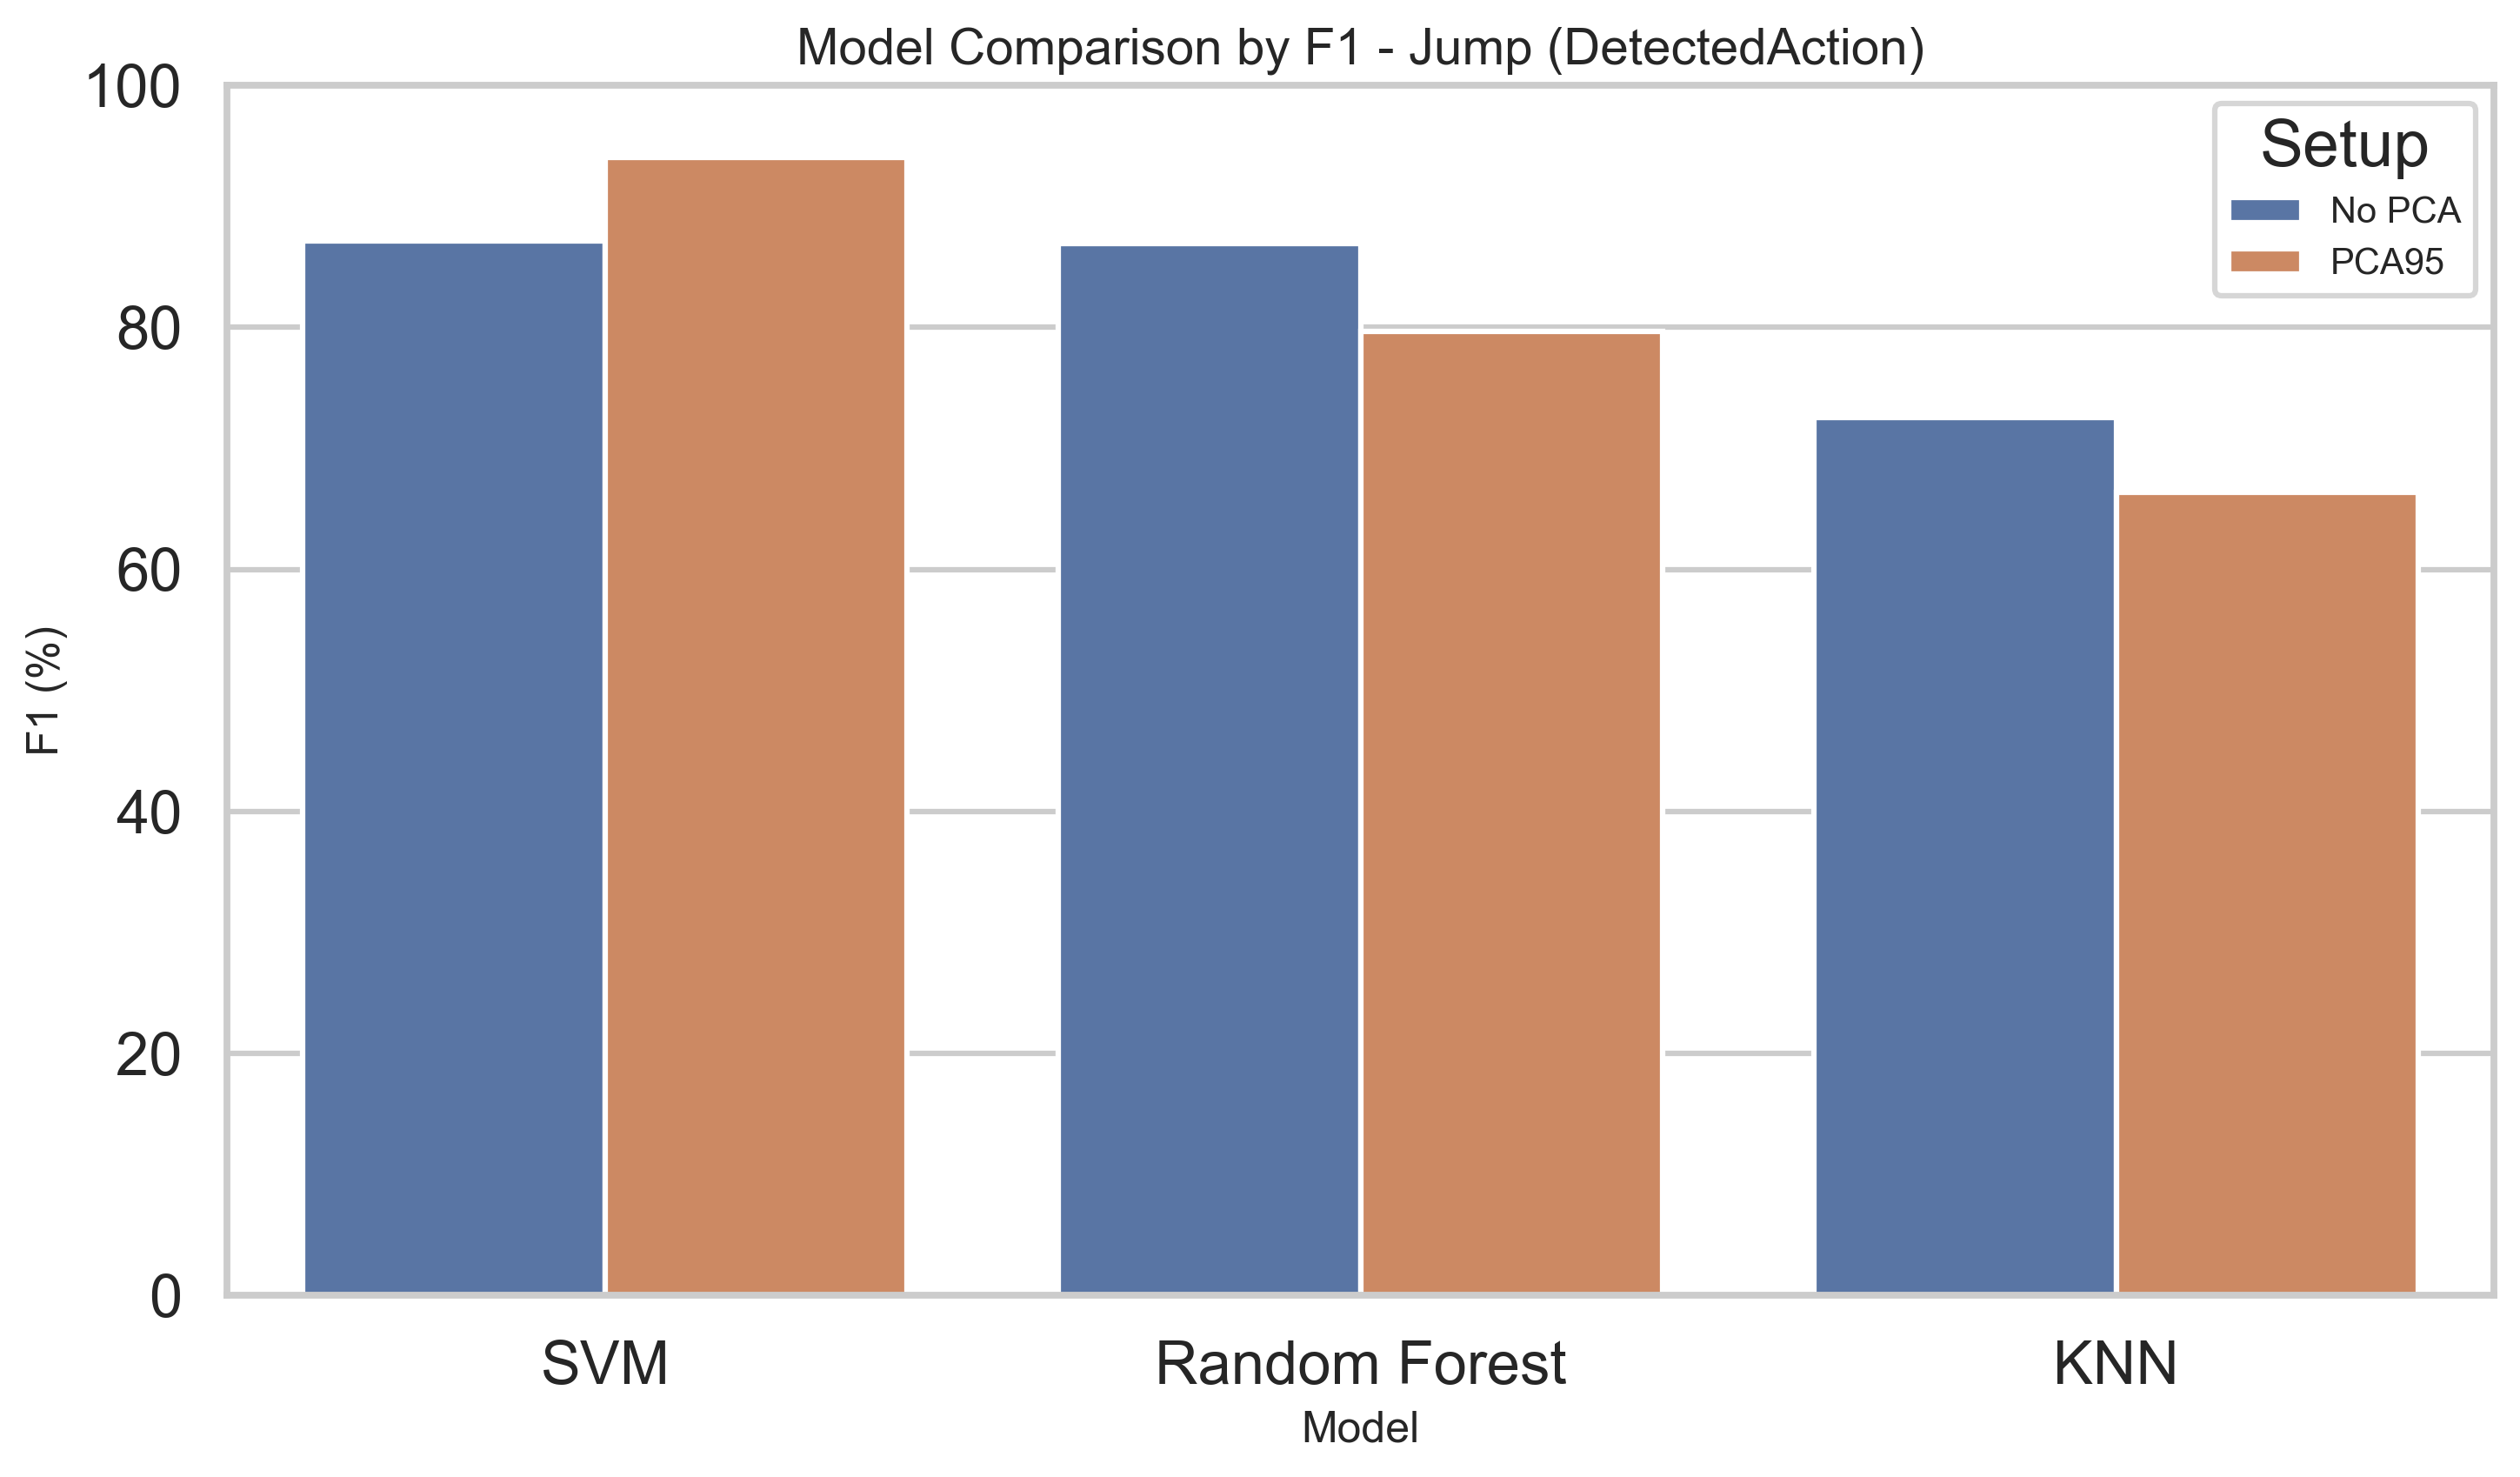
\includegraphics[width=0.85\linewidth]{Images/Generated/TaskResults/Jump/DetectedAction/model_comparison_f1.png}
    \caption{مقایسه عملکرد مدل‌ها بر اساس معیار \lr{F1} در فعالیت پریدن.}
    \label{fig:jump_detectedaction_model_comparison_f1}
\end{figure}

\noindent\textbf{توضیح شکل:} این نمودار اثر استفاده یا عدم استفاده از کاهش بعد را برای هر مدل نشان می‌دهد.
\vspace{0.8em}

\begin{figure}[H]
    \centering
    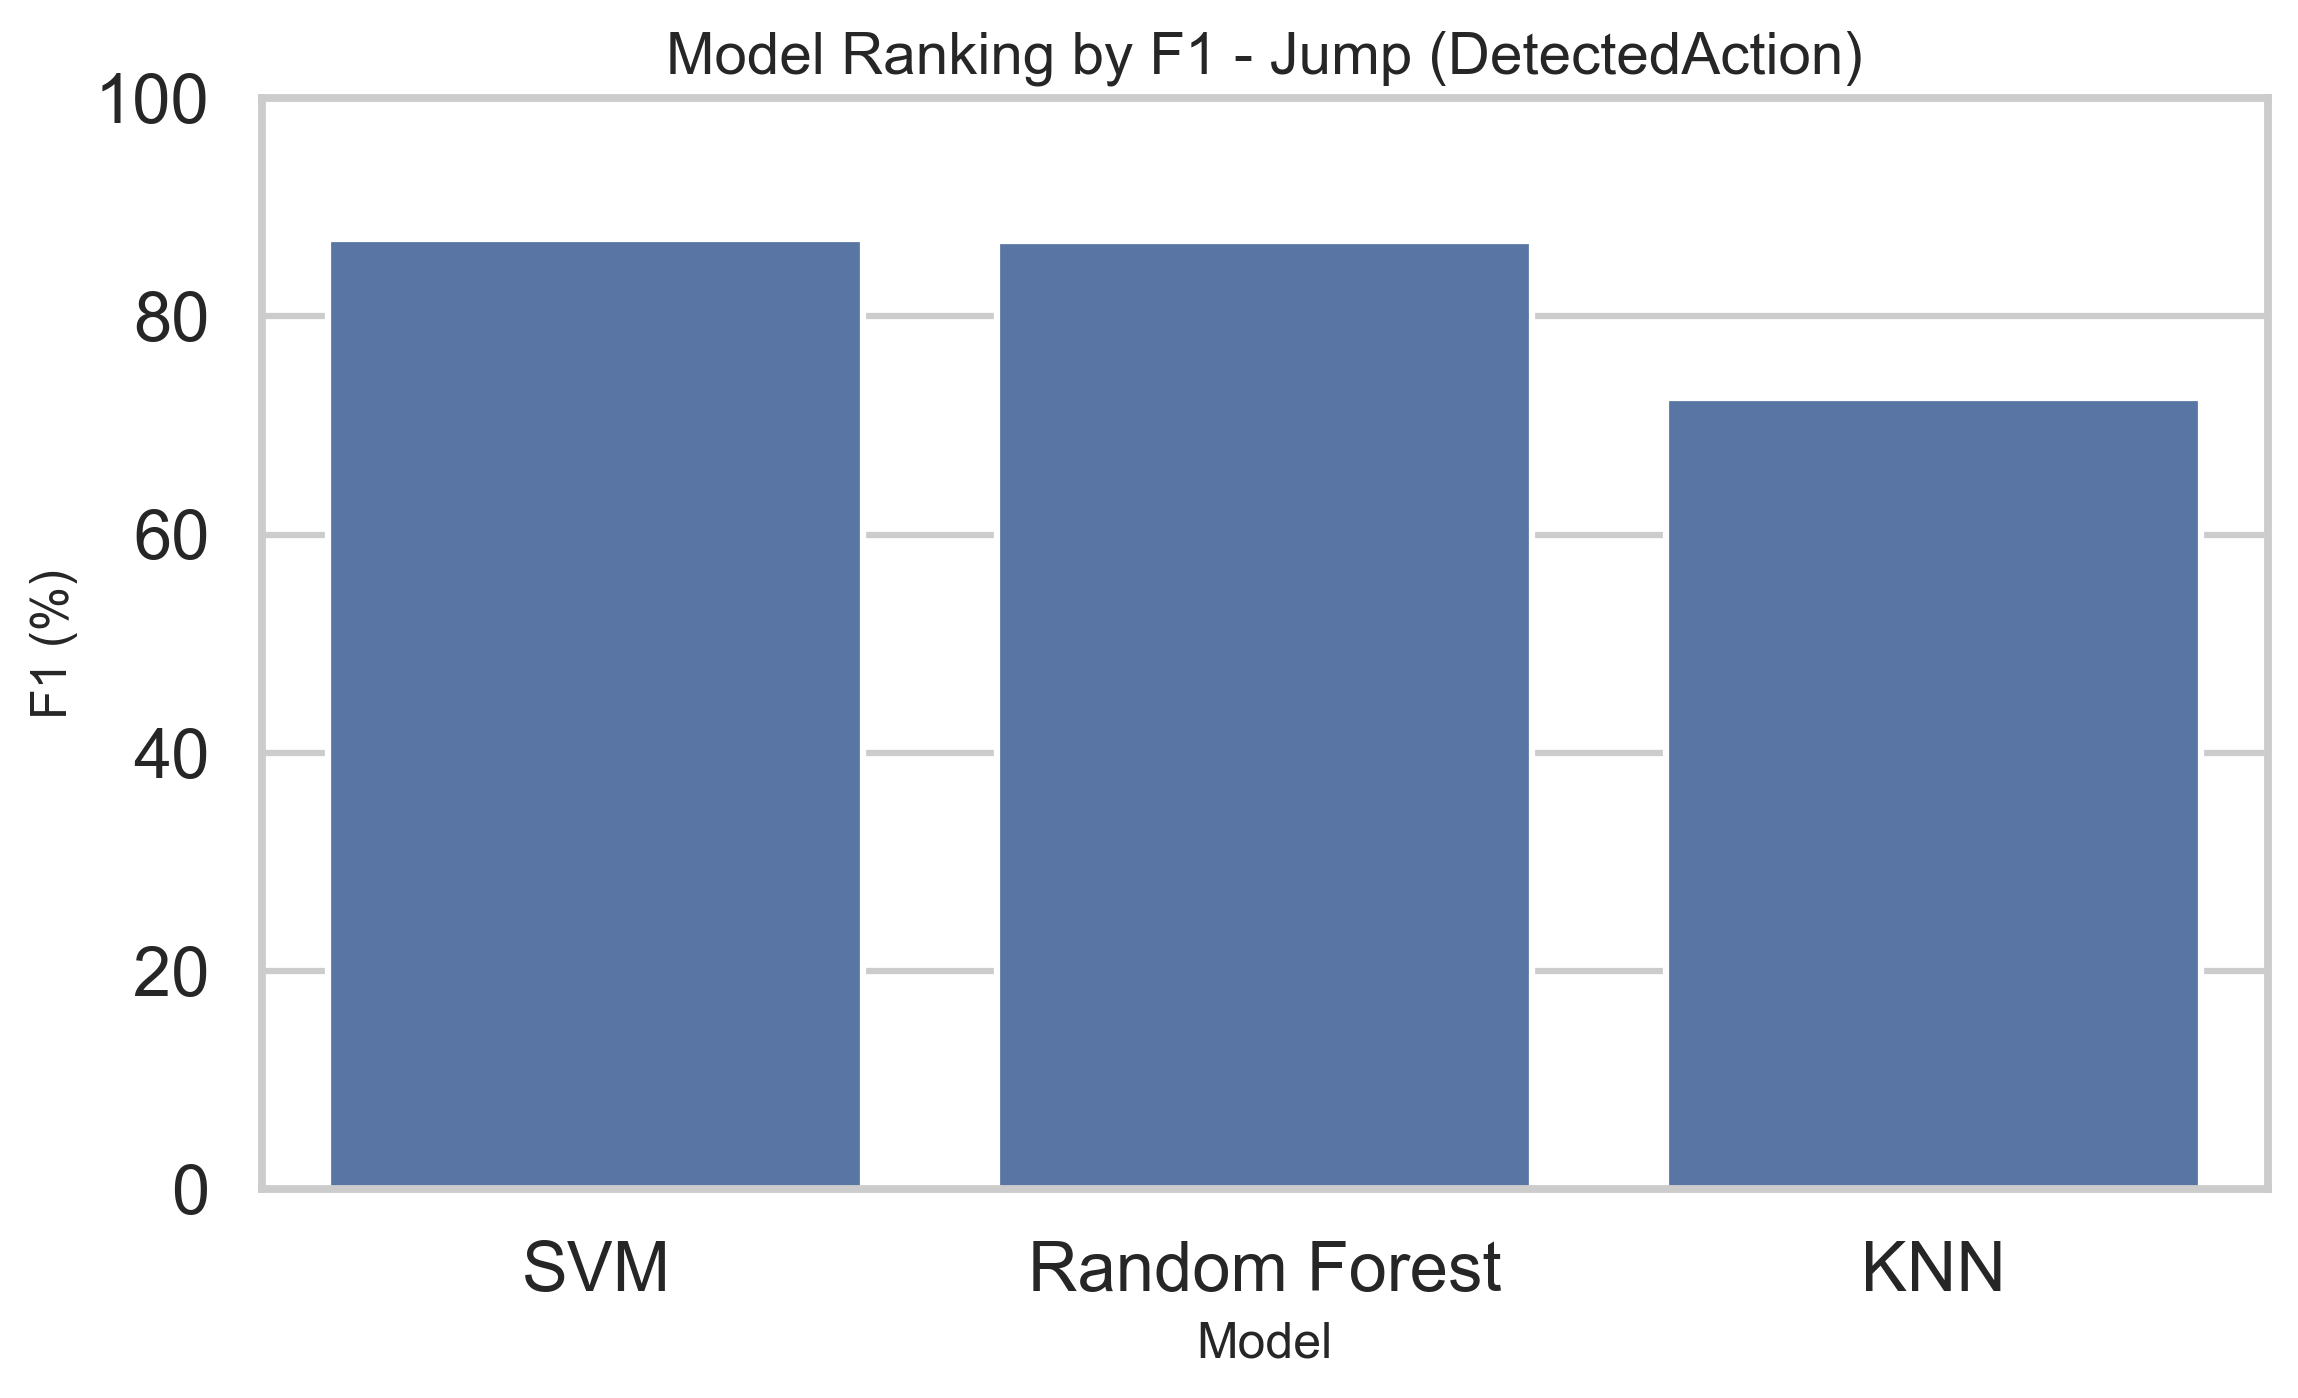
\includegraphics[width=0.85\linewidth]{Images/Generated/TaskResults/Jump/DetectedAction/model_ranking_f1.png}
    \caption{رتبه‌بندی مدل‌ها بر اساس معیار \lr{F1} در فعالیت پریدن.}
    \label{fig:jump_detectedaction_model_ranking_f1}
\end{figure}

\noindent\textbf{توضیح شکل:} این شکل جمع‌بندی سریعی از برتری نسبی مدل‌ها ارائه می‌دهد.
\vspace{0.8em}

\begin{figure}[H]
    \centering
    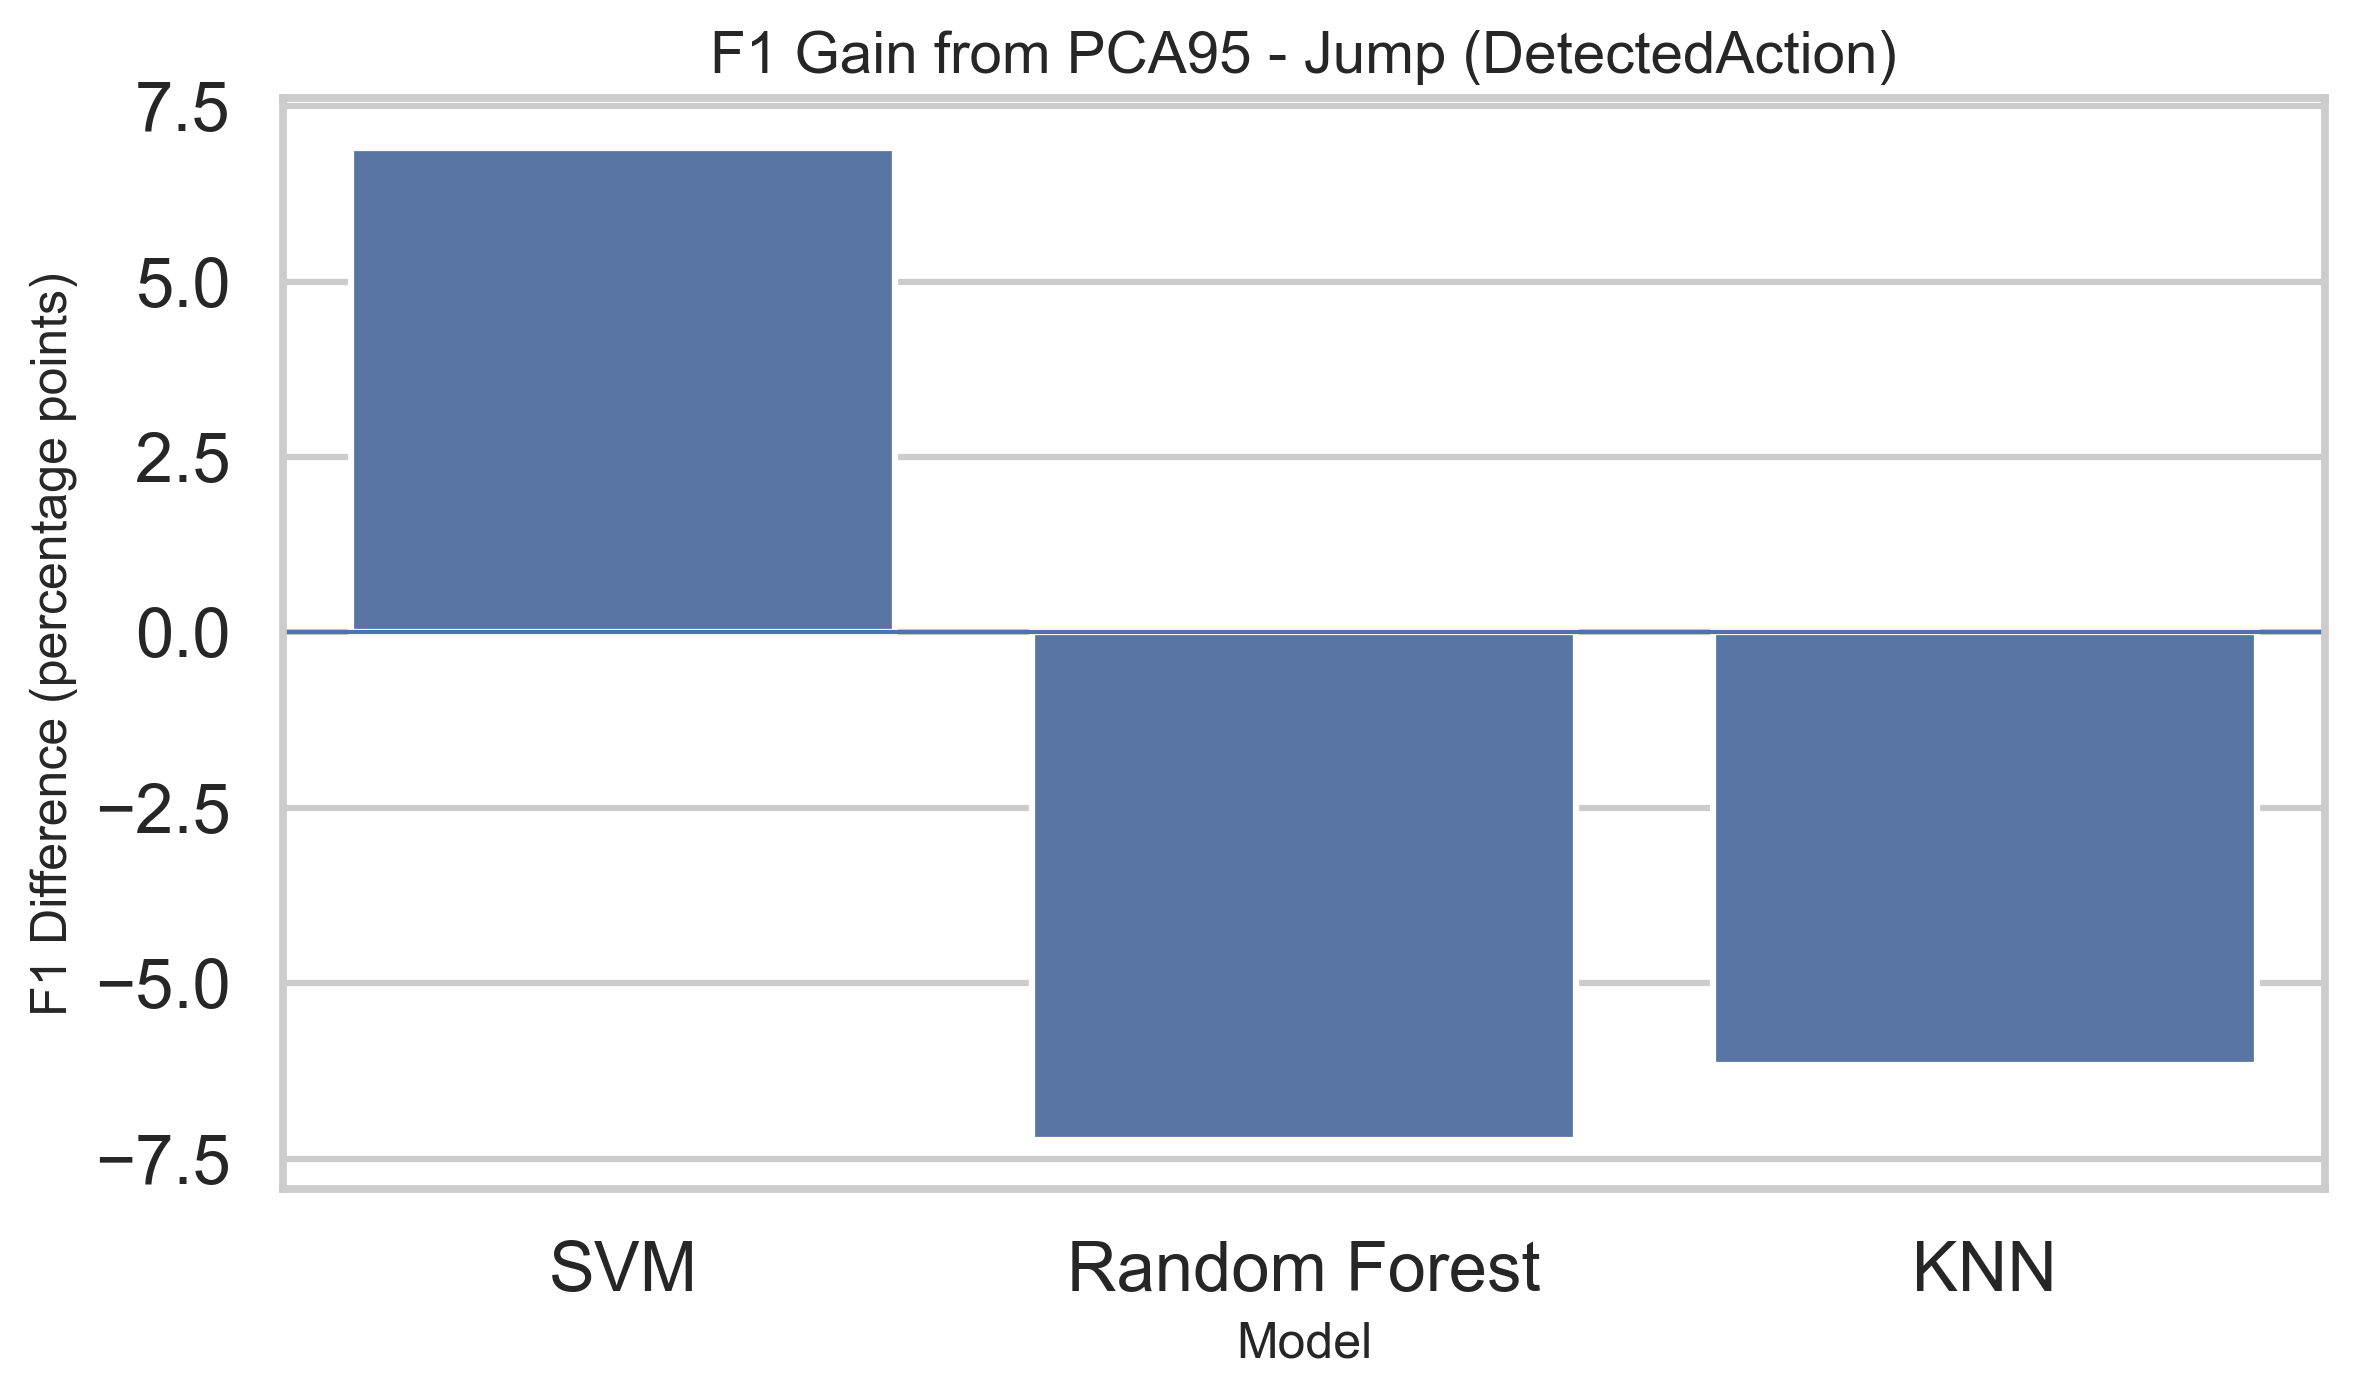
\includegraphics[width=0.85\linewidth]{Images/Generated/TaskResults/Jump/DetectedAction/f1_gain_pca_vs_no_pca.png}
    \caption{تغییر معیار \lr{F1} پس از اعمال \lr{PCA95} در فعالیت پریدن.}
    \label{fig:jump_detectedaction_f1_gain_pca}
\end{figure}

\noindent\textbf{توضیح شکل:} این شکل نشان می‌دهد کاهش بعد برای هر مدل سودمند بوده یا موجب افت عملکرد شده است.
\vspace{0.8em}

\begin{figure}[H]
    \centering
    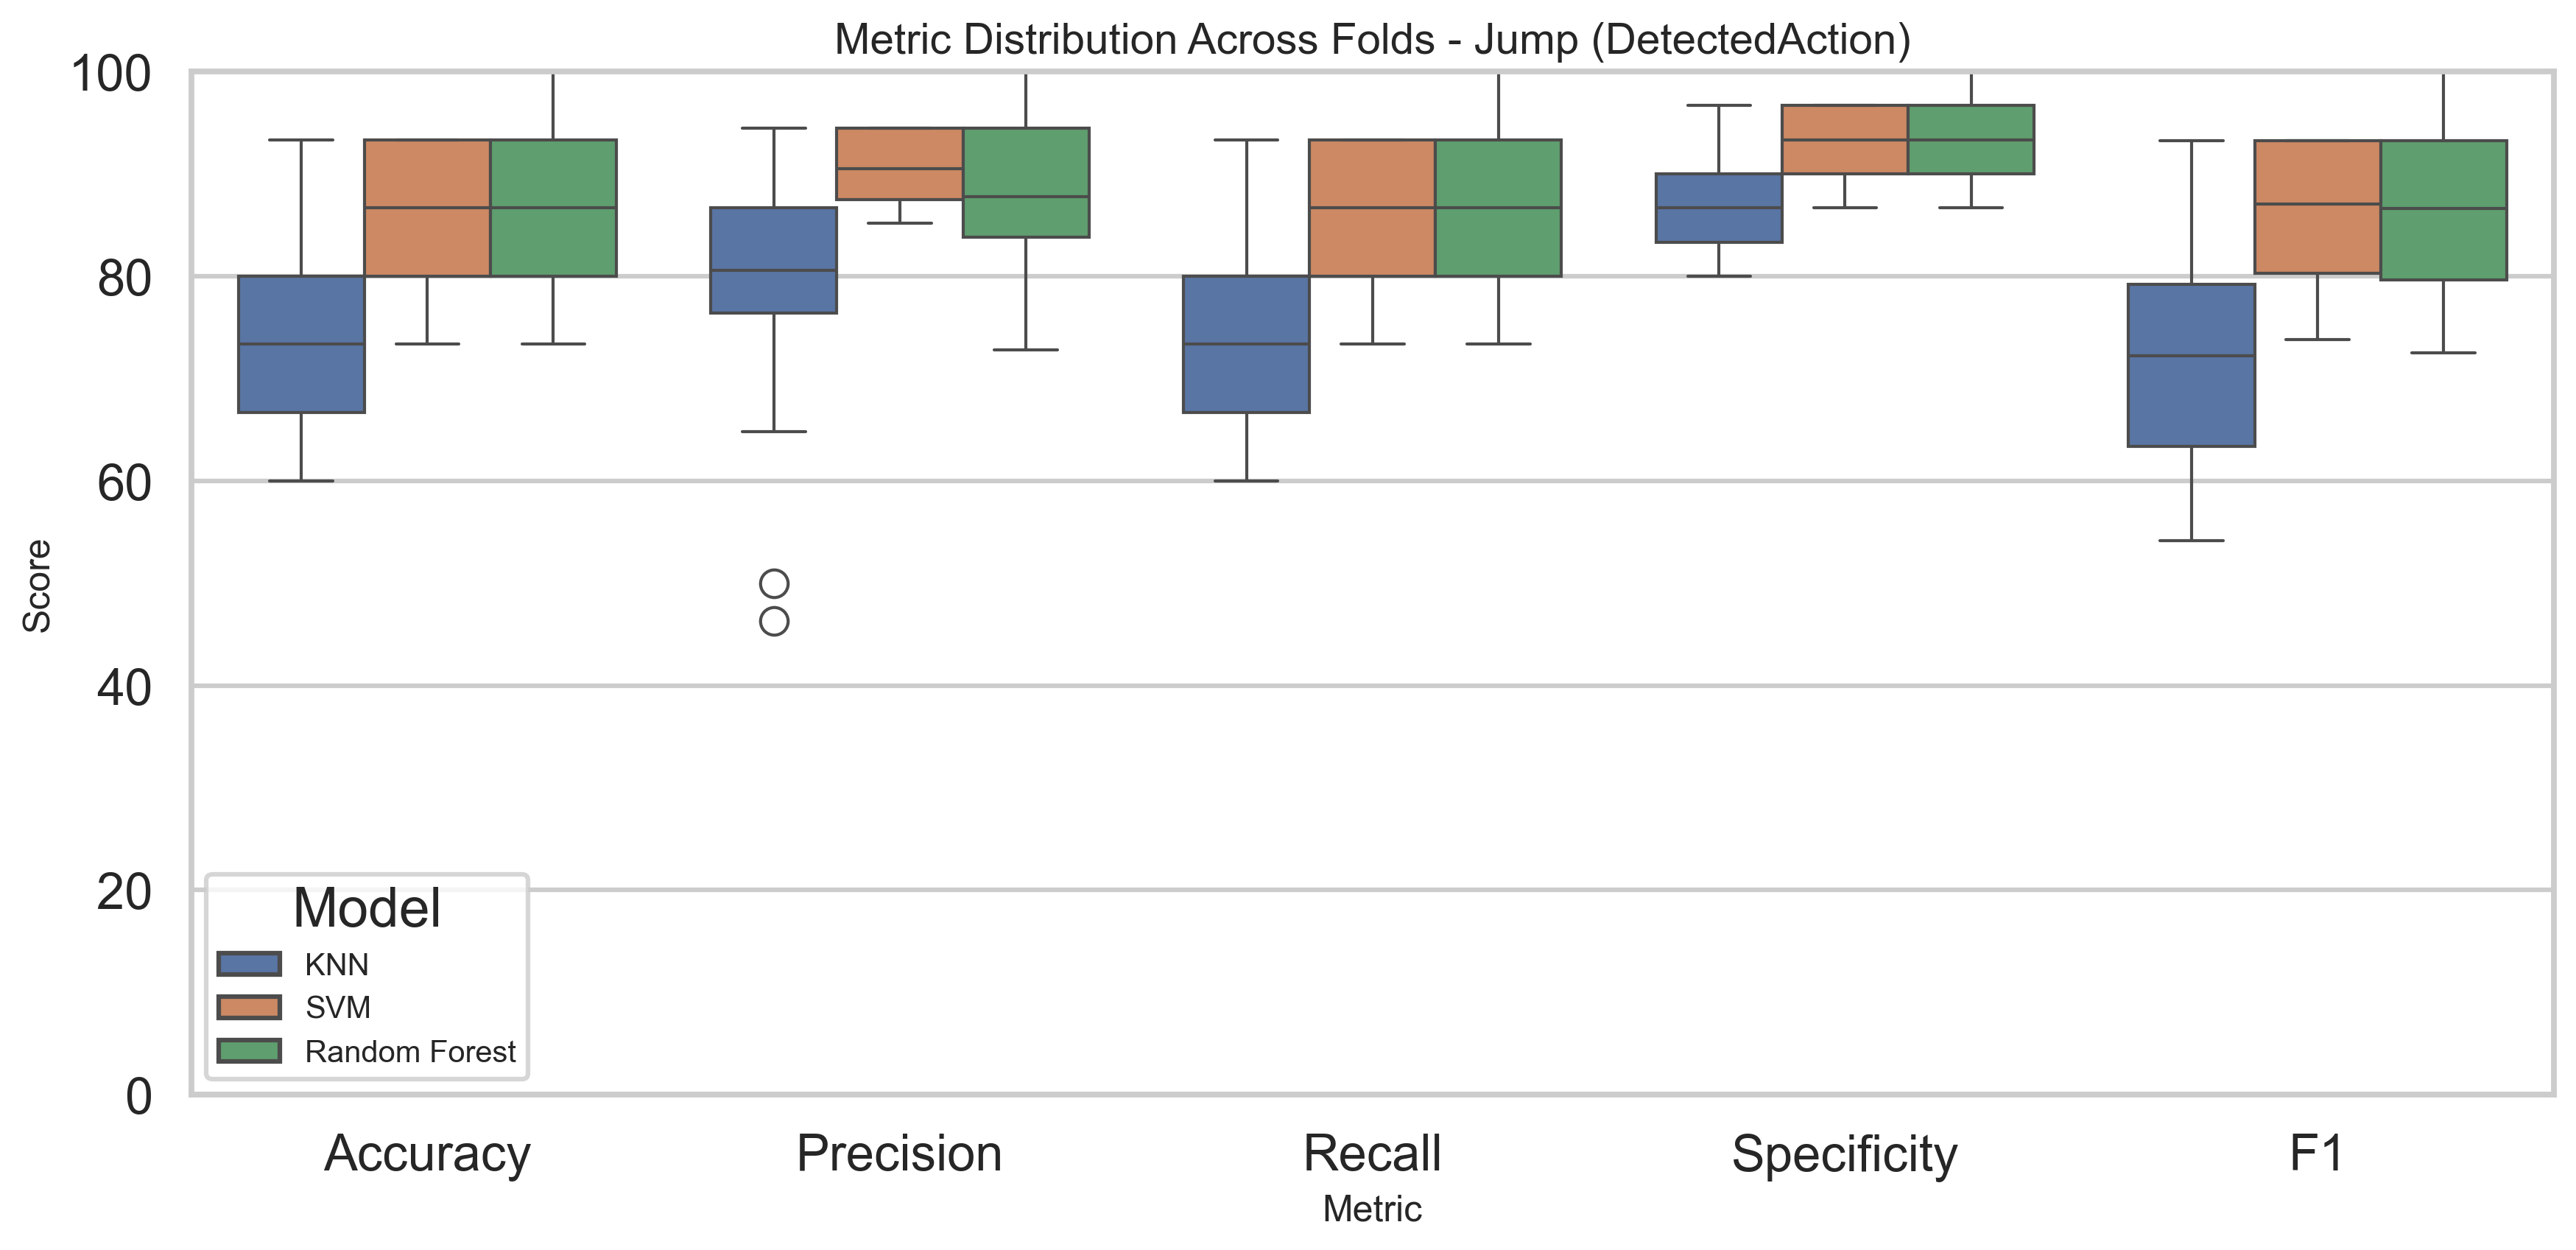
\includegraphics[width=0.85\linewidth]{Images/Generated/TaskResults/Jump/DetectedAction/metric_boxplots.png}
    \caption{پراکندگی معیارهای ارزیابی در تکرارهای اعتبارسنجی برای فعالیت پریدن.}
    \label{fig:jump_detectedaction_metric_boxplots}
\end{figure}

\noindent\textbf{توضیح شکل:} این شکل پایداری مدل‌ها را در foldهای مختلف نشان می‌دهد.
\vspace{0.8em}

\begin{figure}[H]
    \centering
    
\includegraphics[width=0.85\linewidth]{Images/Generated/TaskResults/Jump/DetectedAction/confusion_matrices_no_pca.png}
    \caption{ماتریس درهم‌ریختگی نرمال‌شده مدل‌ها در فعالیت پریدن (no_pca).}
    \label{fig:jump_detectedaction_confusion_no_pca}
\end{figure}

\noindent\textbf{توضیح شکل:} این شکل مشخص می‌کند خطاهای اصلی بین کدام کلاس‌های عملکردی رخ داده است.
\vspace{0.8em}

\begin{figure}[H]
    \centering
    
\includegraphics[width=0.85\linewidth]{Images/Generated/TaskResults/Jump/DetectedAction/per_class_recall_no_pca.png}
    \caption{مقایسه \lr{Recall} هر کلاس در فعالیت پریدن (no_pca).}
    \label{fig:jump_detectedaction_per_class_recall_no_pca}
\end{figure}

\noindent\textbf{توضیح شکل:} این نمودار حساسیت مدل‌ها نسبت به هر سطح عملکردی را نشان می‌دهد.
\vspace{0.8em}

\begin{figure}[H]
    \centering
    
\includegraphics[width=0.85\linewidth]{Images/Generated/TaskResults/Jump/DetectedAction/confusion_matrices_pca95.png}
    \caption{ماتریس درهم‌ریختگی نرمال‌شده مدل‌ها در فعالیت پریدن (pca95).}
    \label{fig:jump_detectedaction_confusion_pca95}
\end{figure}

\noindent\textbf{توضیح شکل:} این شکل مشخص می‌کند خطاهای اصلی بین کدام کلاس‌های عملکردی رخ داده است.
\vspace{0.8em}

\begin{figure}[H]
    \centering
    
\includegraphics[width=0.85\linewidth]{Images/Generated/TaskResults/Jump/DetectedAction/per_class_recall_pca95.png}
    \caption{مقایسه \lr{Recall} هر کلاس در فعالیت پریدن (pca95).}
    \label{fig:jump_detectedaction_per_class_recall_pca95}
\end{figure}

\noindent\textbf{توضیح شکل:} این نمودار حساسیت مدل‌ها نسبت به هر سطح عملکردی را نشان می‌دهد.
\vspace{0.8em}

\begin{figure}[H]
    \centering
    
\includegraphics[width=0.85\linewidth]{Images/Generated/TaskResults/Jump/DetectedAction/rf_top_feature_importance.png}
    \caption{20 ویژگی برتر بر اساس اهمیت در مدل \lr{Random Forest} برای فعالیت پریدن.}
    \label{fig:jump_detectedaction_rf_importance}
\end{figure}

\noindent\textbf{توضیح شکل:} این شکل نشان می‌دهد کدام حسگرها، محورها و شاخص‌های آماری نقش بیشتری در تصمیم‌گیری مدل داشته‌اند.
\vspace{0.8em}

\begin{figure}[H]
    \centering
    
\includegraphics[width=0.85\linewidth]{Images/Generated/TaskResults/Jump/DetectedAction/class_centroid_feature_heatmap.png}
    \caption{میانگین نرمال‌شده ویژگی‌های برتر در کلاس‌های مختلف فعالیت پریدن.}
    \label{fig:jump_detectedaction_class_centroid_heatmap}
\end{figure}

\noindent\textbf{توضیح شکل:} این نقشه حرارتی الگوی میانگین ویژگی‌ها را در هر سطح عملکردی نمایش می‌دهد.
\vspace{0.8em}

\begin{figure}[H]
    \centering
    
\includegraphics[width=0.85\linewidth]{Images/Generated/TaskResults/Jump/DetectedAction/svm_metrics_vs_pca_components.png}
    \caption{تغییر عملکرد مدل \lr{SVM} نسبت به تعداد مؤلفه‌های اصلی در فعالیت پریدن.}
    \label{fig:jump_detectedaction_svm_metrics_vs_pca_components}
\end{figure}

\noindent\textbf{توضیح شکل:} این نمودار برای انتخاب بازه مناسب تعداد مؤلفه‌های اصلی استفاده می‌شود.
\vspace{0.8em}

\begin{figure}[H]
    \centering
    
\includegraphics[width=0.85\linewidth]{Images/Generated/TaskResults/Jump/DetectedAction/models_f1_vs_pca_components.png}
    \caption{مقایسه مدل‌ها نسبت به تعداد مؤلفه‌های اصلی در فعالیت پریدن.}
    \label{fig:jump_detectedaction_models_f1_vs_pca_components}
\end{figure}

\noindent\textbf{توضیح شکل:} این نمودار نشان می‌دهد انتخاب تعداد مؤلفه‌ها و انتخاب مدل باید هم‌زمان انجام شود.
\vspace{0.8em}


\subsection*{نمودارهای فعالیت ایستادن}

\subsubsection*{داده‌های اصلی}

\begin{figure}[H]
    \centering
    
\includegraphics[width=0.85\linewidth]{Images/Generated/TaskResults/Stand/Normal/signal_sample.png}
    \caption{نمونه سیگنال‌های ثبت‌شده در فعالیت ایستادن (داده‌های اصلی).}
    \label{fig:stand_normal_signal_sample}
\end{figure}

\noindent\textbf{توضیح شکل:} این شکل نمایی از ماهیت زمانی سیگنال‌های حسگرها را برای فعالیت مورد نظر نشان می‌دهد.
\vspace{0.8em}

\begin{figure}[H]
    \centering
    
\includegraphics[width=0.85\linewidth]{Images/Generated/TaskResults/Stand/Normal/class_distribution.png}
    \caption{توزیع تعداد نمونه‌ها در سطوح عملکردی فعالیت ایستادن.}
    \label{fig:stand_normal_class_distribution}
\end{figure}

\noindent\textbf{توضیح شکل:} این نمودار برای بررسی تعادل داده‌ها بین کلاس‌های صفر، یک و دو استفاده می‌شود.
\vspace{0.8em}

\begin{figure}[H]
    \centering
    
\includegraphics[width=0.85\linewidth]{Images/Generated/TaskResults/Stand/Normal/feature_correlation_heatmap.png}
    \caption{نقشه همبستگی 20 ویژگی با بیشترین واریانس در فعالیت ایستادن.}
    \label{fig:stand_normal_feature_correlation}
\end{figure}

\noindent\textbf{توضیح شکل:} این نمودار وجود اطلاعات تکراری در فضای ویژگی را نشان می‌دهد و استفاده از کاهش بعد را توجیه می‌کند.
\vspace{0.8em}

\begin{figure}[H]
    \centering
    
\includegraphics[width=0.85\linewidth]{Images/Generated/TaskResults/Stand/Normal/pca_variance_curve.png}
    \caption{درصد واریانس توضیح‌داده‌شده و واریانس تجمعی مؤلفه‌های اصلی در فعالیت ایستادن.}
    \label{fig:stand_normal_pca_variance}
\end{figure}

\noindent\textbf{توضیح شکل:} این شکل مبنای انتخاب آستانه ۹۵ درصد و تعیین تعداد مؤلفه‌های نگه‌داشته‌شده را نشان می‌دهد.
\vspace{0.8em}

\begin{figure}[H]
    \centering
    
\includegraphics[width=0.85\linewidth]{Images/Generated/TaskResults/Stand/Normal/pca_scatter_pc1_pc2.png}
    \caption{پراکندگی نمونه‌های فعالیت ایستادن در فضای دو مؤلفه اصلی اول.}
    \label{fig:stand_normal_pca_scatter}
\end{figure}

\noindent\textbf{توضیح شکل:} این شکل یک تصویر اولیه از جدایی یا هم‌پوشانی کلاس‌ها در فضای کاهش‌یافته ارائه می‌دهد.
\vspace{0.8em}

\begin{figure}[H]
    \centering
    
\includegraphics[width=0.85\linewidth]{Images/Generated/TaskResults/Stand/Normal/model_comparison_f1.png}
    \caption{مقایسه عملکرد مدل‌ها بر اساس معیار \lr{F1} در فعالیت ایستادن.}
    \label{fig:stand_normal_model_comparison_f1}
\end{figure}

\noindent\textbf{توضیح شکل:} این نمودار اثر استفاده یا عدم استفاده از کاهش بعد را برای هر مدل نشان می‌دهد.
\vspace{0.8em}

\begin{figure}[H]
    \centering
    
\includegraphics[width=0.85\linewidth]{Images/Generated/TaskResults/Stand/Normal/model_ranking_f1.png}
    \caption{رتبه‌بندی مدل‌ها بر اساس معیار \lr{F1} در فعالیت ایستادن.}
    \label{fig:stand_normal_model_ranking_f1}
\end{figure}

\noindent\textbf{توضیح شکل:} این شکل جمع‌بندی سریعی از برتری نسبی مدل‌ها ارائه می‌دهد.
\vspace{0.8em}

\begin{figure}[H]
    \centering
    
\includegraphics[width=0.85\linewidth]{Images/Generated/TaskResults/Stand/Normal/f1_gain_pca_vs_no_pca.png}
    \caption{تغییر معیار \lr{F1} پس از اعمال \lr{PCA95} در فعالیت ایستادن.}
    \label{fig:stand_normal_f1_gain_pca}
\end{figure}

\noindent\textbf{توضیح شکل:} این شکل نشان می‌دهد کاهش بعد برای هر مدل سودمند بوده یا موجب افت عملکرد شده است.
\vspace{0.8em}

\begin{figure}[H]
    \centering
    
\includegraphics[width=0.85\linewidth]{Images/Generated/TaskResults/Stand/Normal/metric_boxplots.png}
    \caption{پراکندگی معیارهای ارزیابی در تکرارهای اعتبارسنجی برای فعالیت ایستادن.}
    \label{fig:stand_normal_metric_boxplots}
\end{figure}

\noindent\textbf{توضیح شکل:} این شکل پایداری مدل‌ها را در foldهای مختلف نشان می‌دهد.
\vspace{0.8em}

\begin{figure}[H]
    \centering
    
\includegraphics[width=0.85\linewidth]{Images/Generated/TaskResults/Stand/Normal/confusion_matrices_no_pca.png}
    \caption{ماتریس درهم‌ریختگی نرمال‌شده مدل‌ها در فعالیت ایستادن (no_pca).}
    \label{fig:stand_normal_confusion_no_pca}
\end{figure}

\noindent\textbf{توضیح شکل:} این شکل مشخص می‌کند خطاهای اصلی بین کدام کلاس‌های عملکردی رخ داده است.
\vspace{0.8em}

\begin{figure}[H]
    \centering
    
\includegraphics[width=0.85\linewidth]{Images/Generated/TaskResults/Stand/Normal/per_class_recall_no_pca.png}
    \caption{مقایسه \lr{Recall} هر کلاس در فعالیت ایستادن (no_pca).}
    \label{fig:stand_normal_per_class_recall_no_pca}
\end{figure}

\noindent\textbf{توضیح شکل:} این نمودار حساسیت مدل‌ها نسبت به هر سطح عملکردی را نشان می‌دهد.
\vspace{0.8em}

\begin{figure}[H]
    \centering
    
\includegraphics[width=0.85\linewidth]{Images/Generated/TaskResults/Stand/Normal/confusion_matrices_pca95.png}
    \caption{ماتریس درهم‌ریختگی نرمال‌شده مدل‌ها در فعالیت ایستادن (pca95).}
    \label{fig:stand_normal_confusion_pca95}
\end{figure}

\noindent\textbf{توضیح شکل:} این شکل مشخص می‌کند خطاهای اصلی بین کدام کلاس‌های عملکردی رخ داده است.
\vspace{0.8em}

\begin{figure}[H]
    \centering
    
\includegraphics[width=0.85\linewidth]{Images/Generated/TaskResults/Stand/Normal/per_class_recall_pca95.png}
    \caption{مقایسه \lr{Recall} هر کلاس در فعالیت ایستادن (pca95).}
    \label{fig:stand_normal_per_class_recall_pca95}
\end{figure}

\noindent\textbf{توضیح شکل:} این نمودار حساسیت مدل‌ها نسبت به هر سطح عملکردی را نشان می‌دهد.
\vspace{0.8em}

\begin{figure}[H]
    \centering
    
\includegraphics[width=0.85\linewidth]{Images/Generated/TaskResults/Stand/Normal/rf_top_feature_importance.png}
    \caption{20 ویژگی برتر بر اساس اهمیت در مدل \lr{Random Forest} برای فعالیت ایستادن.}
    \label{fig:stand_normal_rf_importance}
\end{figure}

\noindent\textbf{توضیح شکل:} این شکل نشان می‌دهد کدام حسگرها، محورها و شاخص‌های آماری نقش بیشتری در تصمیم‌گیری مدل داشته‌اند.
\vspace{0.8em}

\begin{figure}[H]
    \centering
    
\includegraphics[width=0.85\linewidth]{Images/Generated/TaskResults/Stand/Normal/class_centroid_feature_heatmap.png}
    \caption{میانگین نرمال‌شده ویژگی‌های برتر در کلاس‌های مختلف فعالیت ایستادن.}
    \label{fig:stand_normal_class_centroid_heatmap}
\end{figure}

\noindent\textbf{توضیح شکل:} این نقشه حرارتی الگوی میانگین ویژگی‌ها را در هر سطح عملکردی نمایش می‌دهد.
\vspace{0.8em}

\begin{figure}[H]
    \centering
    
\includegraphics[width=0.85\linewidth]{Images/Generated/TaskResults/Stand/Normal/svm_metrics_vs_pca_components.png}
    \caption{تغییر عملکرد مدل \lr{SVM} نسبت به تعداد مؤلفه‌های اصلی در فعالیت ایستادن.}
    \label{fig:stand_normal_svm_metrics_vs_pca_components}
\end{figure}

\noindent\textbf{توضیح شکل:} این نمودار برای انتخاب بازه مناسب تعداد مؤلفه‌های اصلی استفاده می‌شود.
\vspace{0.8em}

\begin{figure}[H]
    \centering
    
\includegraphics[width=0.85\linewidth]{Images/Generated/TaskResults/Stand/Normal/models_f1_vs_pca_components.png}
    \caption{مقایسه مدل‌ها نسبت به تعداد مؤلفه‌های اصلی در فعالیت ایستادن.}
    \label{fig:stand_normal_models_f1_vs_pca_components}
\end{figure}

\noindent\textbf{توضیح شکل:} این نمودار نشان می‌دهد انتخاب تعداد مؤلفه‌ها و انتخاب مدل باید هم‌زمان انجام شود.
\vspace{0.8em}

\subsection*{نمودارهای فعالیت بلند شدن از صندلی}

\subsubsection*{داده‌های اصلی}

\begin{figure}[H]
    \centering
    
\includegraphics[width=0.85\linewidth]{Images/Generated/TaskResults/Sit_To_Stand/Normal/signal_sample.png}
    \caption{نمونه سیگنال‌های ثبت‌شده در فعالیت بلند شدن از صندلی (داده‌های اصلی).}
    \label{fig:sit_to_stand_normal_signal_sample}
\end{figure}

\noindent\textbf{توضیح شکل:} این شکل نمایی از ماهیت زمانی سیگنال‌های حسگرها را برای فعالیت مورد نظر نشان می‌دهد.
\vspace{0.8em}

\begin{figure}[H]
    \centering
    
\includegraphics[width=0.85\linewidth]{Images/Generated/TaskResults/Sit_To_Stand/Normal/class_distribution.png}
    \caption{توزیع تعداد نمونه‌ها در سطوح عملکردی فعالیت بلند شدن از صندلی.}
    \label{fig:sit_to_stand_normal_class_distribution}
\end{figure}

\noindent\textbf{توضیح شکل:} این نمودار برای بررسی تعادل داده‌ها بین کلاس‌های صفر، یک و دو استفاده می‌شود.
\vspace{0.8em}

\begin{figure}[H]
    \centering
    
\includegraphics[width=0.85\linewidth]{Images/Generated/TaskResults/Sit_To_Stand/Normal/feature_correlation_heatmap.png}
    \caption{نقشه همبستگی 20 ویژگی با بیشترین واریانس در فعالیت بلند شدن از صندلی.}
    \label{fig:sit_to_stand_normal_feature_correlation}
\end{figure}

\noindent\textbf{توضیح شکل:} این نمودار وجود اطلاعات تکراری در فضای ویژگی را نشان می‌دهد و استفاده از کاهش بعد را توجیه می‌کند.
\vspace{0.8em}

\begin{figure}[H]
    \centering
    
\includegraphics[width=0.85\linewidth]{Images/Generated/TaskResults/Sit_To_Stand/Normal/pca_variance_curve.png}
    \caption{درصد واریانس توضیح‌داده‌شده و واریانس تجمعی مؤلفه‌های اصلی در فعالیت بلند شدن از صندلی.}
    \label{fig:sit_to_stand_normal_pca_variance}
\end{figure}

\noindent\textbf{توضیح شکل:} این شکل مبنای انتخاب آستانه ۹۵ درصد و تعیین تعداد مؤلفه‌های نگه‌داشته‌شده را نشان می‌دهد.
\vspace{0.8em}

\begin{figure}[H]
    \centering
    
\includegraphics[width=0.85\linewidth]{Images/Generated/TaskResults/Sit_To_Stand/Normal/pca_scatter_pc1_pc2.png}
    \caption{پراکندگی نمونه‌های فعالیت بلند شدن از صندلی در فضای دو مؤلفه اصلی اول.}
    \label{fig:sit_to_stand_normal_pca_scatter}
\end{figure}

\noindent\textbf{توضیح شکل:} این شکل یک تصویر اولیه از جدایی یا هم‌پوشانی کلاس‌ها در فضای کاهش‌یافته ارائه می‌دهد.
\vspace{0.8em}

\begin{figure}[H]
    \centering
    
\includegraphics[width=0.85\linewidth]{Images/Generated/TaskResults/Sit_To_Stand/Normal/model_comparison_f1.png}
    \caption{مقایسه عملکرد مدل‌ها بر اساس معیار \lr{F1} در فعالیت بلند شدن از صندلی.}
    \label{fig:sit_to_stand_normal_model_comparison_f1}
\end{figure}

\noindent\textbf{توضیح شکل:} این نمودار اثر استفاده یا عدم استفاده از کاهش بعد را برای هر مدل نشان می‌دهد.
\vspace{0.8em}

\begin{figure}[H]
    \centering
    
\includegraphics[width=0.85\linewidth]{Images/Generated/TaskResults/Sit_To_Stand/Normal/model_ranking_f1.png}
    \caption{رتبه‌بندی مدل‌ها بر اساس معیار \lr{F1} در فعالیت بلند شدن از صندلی.}
    \label{fig:sit_to_stand_normal_model_ranking_f1}
\end{figure}

\noindent\textbf{توضیح شکل:} این شکل جمع‌بندی سریعی از برتری نسبی مدل‌ها ارائه می‌دهد.
\vspace{0.8em}

\begin{figure}[H]
    \centering
    
\includegraphics[width=0.85\linewidth]{Images/Generated/TaskResults/Sit_To_Stand/Normal/f1_gain_pca_vs_no_pca.png}
    \caption{تغییر معیار \lr{F1} پس از اعمال \lr{PCA95} در فعالیت بلند شدن از صندلی.}
    \label{fig:sit_to_stand_normal_f1_gain_pca}
\end{figure}

\noindent\textbf{توضیح شکل:} این شکل نشان می‌دهد کاهش بعد برای هر مدل سودمند بوده یا موجب افت عملکرد شده است.
\vspace{0.8em}

\begin{figure}[H]
    \centering
    
\includegraphics[width=0.85\linewidth]{Images/Generated/TaskResults/Sit_To_Stand/Normal/metric_boxplots.png}
    \caption{پراکندگی معیارهای ارزیابی در تکرارهای اعتبارسنجی برای فعالیت بلند شدن از صندلی.}
    \label{fig:sit_to_stand_normal_metric_boxplots}
\end{figure}

\noindent\textbf{توضیح شکل:} این شکل پایداری مدل‌ها را در foldهای مختلف نشان می‌دهد.
\vspace{0.8em}

\begin{figure}[H]
    \centering
    
\includegraphics[width=0.85\linewidth]{Images/Generated/TaskResults/Sit_To_Stand/Normal/confusion_matrices_no_pca.png}
    \caption{ماتریس درهم‌ریختگی نرمال‌شده مدل‌ها در فعالیت بلند شدن از صندلی (no_pca).}
    \label{fig:sit_to_stand_normal_confusion_no_pca}
\end{figure}

\noindent\textbf{توضیح شکل:} این شکل مشخص می‌کند خطاهای اصلی بین کدام کلاس‌های عملکردی رخ داده است.
\vspace{0.8em}

\begin{figure}[H]
    \centering
    
\includegraphics[width=0.85\linewidth]{Images/Generated/TaskResults/Sit_To_Stand/Normal/per_class_recall_no_pca.png}
    \caption{مقایسه \lr{Recall} هر کلاس در فعالیت بلند شدن از صندلی (no_pca).}
    \label{fig:sit_to_stand_normal_per_class_recall_no_pca}
\end{figure}

\noindent\textbf{توضیح شکل:} این نمودار حساسیت مدل‌ها نسبت به هر سطح عملکردی را نشان می‌دهد.
\vspace{0.8em}

\begin{figure}[H]
    \centering
    
\includegraphics[width=0.85\linewidth]{Images/Generated/TaskResults/Sit_To_Stand/Normal/confusion_matrices_pca95.png}
    \caption{ماتریس درهم‌ریختگی نرمال‌شده مدل‌ها در فعالیت بلند شدن از صندلی (pca95).}
    \label{fig:sit_to_stand_normal_confusion_pca95}
\end{figure}

\noindent\textbf{توضیح شکل:} این شکل مشخص می‌کند خطاهای اصلی بین کدام کلاس‌های عملکردی رخ داده است.
\vspace{0.8em}

\begin{figure}[H]
    \centering
    
\includegraphics[width=0.85\linewidth]{Images/Generated/TaskResults/Sit_To_Stand/Normal/per_class_recall_pca95.png}
    \caption{مقایسه \lr{Recall} هر کلاس در فعالیت بلند شدن از صندلی (pca95).}
    \label{fig:sit_to_stand_normal_per_class_recall_pca95}
\end{figure}

\noindent\textbf{توضیح شکل:} این نمودار حساسیت مدل‌ها نسبت به هر سطح عملکردی را نشان می‌دهد.
\vspace{0.8em}

\begin{figure}[H]
    \centering
    \includegraphics[width=0.85\linewidth]{Images/Generated/TaskResults/Sit_To_Stand/Normal/rf_top_feature_importance.png}
    \caption{20 ویژگی برتر بر اساس اهمیت در مدل \lr{Random Forest} برای فعالیت بلند شدن از صندلی.}
    \label{fig:sit_to_stand_normal_rf_importance}
\end{figure}

\noindent\textbf{توضیح شکل:} این شکل نشان می‌دهد کدام حسگرها، محورها و شاخص‌های آماری نقش بیشتری در تصمیم‌گیری مدل داشته‌اند.
\vspace{0.8em}

\begin{figure}[H]
    \centering
    \includegraphics[width=0.85\linewidth]{Images/Generated/TaskResults/Sit_To_Stand/Normal/class_centroid_feature_heatmap.png}
    \caption{میانگین نرمال‌شده ویژگی‌های برتر در کلاس‌های مختلف فعالیت بلند شدن از صندلی.}
    \label{fig:sit_to_stand_normal_class_centroid_heatmap}
\end{figure}

\noindent\textbf{توضیح شکل:} این نقشه حرارتی الگوی میانگین ویژگی‌ها را در هر سطح عملکردی نمایش می‌دهد.
\vspace{0.8em}

\begin{figure}[H]
    \centering
    \includegraphics[width=0.85\linewidth]{Images/Generated/TaskResults/Sit_To_Stand/Normal/svm_metrics_vs_pca_components.png}
    \caption{تغییر عملکرد مدل \lr{SVM} نسبت به تعداد مؤلفه‌های اصلی در فعالیت بلند شدن از صندلی.}
    \label{fig:sit_to_stand_normal_svm_metrics_vs_pca_components}
\end{figure}

\noindent\textbf{توضیح شکل:} این نمودار برای انتخاب بازه مناسب تعداد مؤلفه‌های اصلی استفاده می‌شود.
\vspace{0.8em}

\begin{figure}[H]
    \centering
    \includegraphics[width=0.85\linewidth]{Images/Generated/TaskResults/Sit_To_Stand/Normal/models_f1_vs_pca_components.png}
    \caption{مقایسه مدل‌ها نسبت به تعداد مؤلفه‌های اصلی در فعالیت بلند شدن از صندلی.}
    \label{fig:sit_to_stand_normal_models_f1_vs_pca_components}
\end{figure}

\noindent\textbf{توضیح شکل:} این نمودار نشان می‌دهد انتخاب تعداد مؤلفه‌ها و انتخاب مدل باید هم‌زمان انجام شود.
\vspace{0.8em}

\subsubsection*{داده‌های جداسازی‌شده با تشخیص فعالیت}

\begin{figure}[H]
    \centering
    \includegraphics[width=0.85\linewidth]{Images/Generated/TaskResults/Sit_To_Stand/DetectedAction/signal_sample.png}
    \caption{نمونه سیگنال‌های ثبت‌شده در فعالیت بلند شدن از صندلی (داده‌های جداسازی‌شده با تشخیص فعالیت).}
    \label{fig:sit_to_stand_detectedaction_signal_sample}
\end{figure}

\noindent\textbf{توضیح شکل:} این شکل نمایی از ماهیت زمانی سیگنال‌های حسگرها را برای فعالیت مورد نظر نشان می‌دهد.
\vspace{0.8em}

\begin{figure}[H]
    \centering
    \includegraphics[width=0.85\linewidth]{Images/Generated/TaskResults/Sit_To_Stand/DetectedAction/class_distribution.png}
    \caption{توزیع تعداد نمونه‌ها در سطوح عملکردی فعالیت بلند شدن از صندلی.}
    \label{fig:sit_to_stand_detectedaction_class_distribution}
\end{figure}

\noindent\textbf{توضیح شکل:} این نمودار برای بررسی تعادل داده‌ها بین کلاس‌های صفر، یک و دو استفاده می‌شود.
\vspace{0.8em}

\begin{figure}[H]
    \centering
    \includegraphics[width=0.85\linewidth]{Images/Generated/TaskResults/Sit_To_Stand/DetectedAction/feature_correlation_heatmap.png}
    \caption{نقشه همبستگی 20 ویژگی با بیشترین واریانس در فعالیت بلند شدن از صندلی.}
    \label{fig:sit_to_stand_detectedaction_feature_correlation}
\end{figure}

\noindent\textbf{توضیح شکل:} این نمودار وجود اطلاعات تکراری در فضای ویژگی را نشان می‌دهد و استفاده از کاهش بعد را توجیه می‌کند.
\vspace{0.8em}

\begin{figure}[H]
    \centering
    \includegraphics[width=0.85\linewidth]{Images/Generated/TaskResults/Sit_To_Stand/DetectedAction/pca_variance_curve.png}
    \caption{درصد واریانس توضیح‌داده‌شده و واریانس تجمعی مؤلفه‌های اصلی در فعالیت بلند شدن از صندلی.}
    \label{fig:sit_to_stand_detectedaction_pca_variance}
\end{figure}

\noindent\textbf{توضیح شکل:} این شکل مبنای انتخاب آستانه ۹۵ درصد و تعیین تعداد مؤلفه‌های نگه‌داشته‌شده را نشان می‌دهد.
\vspace{0.8em}

\begin{figure}[H]
    \centering
    \includegraphics[width=0.85\linewidth]{Images/Generated/TaskResults/Sit_To_Stand/DetectedAction/pca_scatter_pc1_pc2.png}
    \caption{پراکندگی نمونه‌های فعالیت بلند شدن از صندلی در فضای دو مؤلفه اصلی اول.}
    \label{fig:sit_to_stand_detectedaction_pca_scatter}
\end{figure}

\noindent\textbf{توضیح شکل:} این شکل یک تصویر اولیه از جدایی یا هم‌پوشانی کلاس‌ها در فضای کاهش‌یافته ارائه می‌دهد.
\vspace{0.8em}

\begin{figure}[H]
    \centering
    \includegraphics[width=0.85\linewidth]{Images/Generated/TaskResults/Sit_To_Stand/DetectedAction/model_comparison_f1.png}
    \caption{مقایسه عملکرد مدل‌ها بر اساس معیار \lr{F1} در فعالیت بلند شدن از صندلی.}
    \label{fig:sit_to_stand_detectedaction_model_comparison_f1}
\end{figure}

\noindent\textbf{توضیح شکل:} این نمودار اثر استفاده یا عدم استفاده از کاهش بعد را برای هر مدل نشان می‌دهد.
\vspace{0.8em}

\begin{figure}[H]
    \centering
    \includegraphics[width=0.85\linewidth]{Images/Generated/TaskResults/Sit_To_Stand/DetectedAction/model_ranking_f1.png}
    \caption{رتبه‌بندی مدل‌ها بر اساس معیار \lr{F1} در فعالیت بلند شدن از صندلی.}
    \label{fig:sit_to_stand_detectedaction_model_ranking_f1}
\end{figure}

\noindent\textbf{توضیح شکل:} این شکل جمع‌بندی سریعی از برتری نسبی مدل‌ها ارائه می‌دهد.
\vspace{0.8em}

\begin{figure}[H]
    \centering
    \includegraphics[width=0.85\linewidth]{Images/Generated/TaskResults/Sit_To_Stand/DetectedAction/f1_gain_pca_vs_no_pca.png}
    \caption{تغییر معیار \lr{F1} پس از اعمال \lr{PCA95} در فعالیت بلند شدن از صندلی.}
    \label{fig:sit_to_stand_detectedaction_f1_gain_pca}
\end{figure}

\noindent\textbf{توضیح شکل:} این شکل نشان می‌دهد کاهش بعد برای هر مدل سودمند بوده یا موجب افت عملکرد شده است.
\vspace{0.8em}

\begin{figure}[H]
    \centering
    \includegraphics[width=0.85\linewidth]{Images/Generated/TaskResults/Sit_To_Stand/DetectedAction/metric_boxplots.png}
    \caption{پراکندگی معیارهای ارزیابی در تکرارهای اعتبارسنجی برای فعالیت بلند شدن از صندلی.}
    \label{fig:sit_to_stand_detectedaction_metric_boxplots}
\end{figure}

\noindent\textbf{توضیح شکل:} این شکل پایداری مدل‌ها را در foldهای مختلف نشان می‌دهد.
\vspace{0.8em}

\begin{figure}[H]
    \centering
    \includegraphics[width=0.85\linewidth]{Images/Generated/TaskResults/Sit_To_Stand/DetectedAction/confusion_matrices_no_pca.png}
    \caption{ماتریس درهم‌ریختگی نرمال‌شده مدل‌ها در فعالیت بلند شدن از صندلی (no_pca).}
    \label{fig:sit_to_stand_detectedaction_confusion_no_pca}
\end{figure}

\noindent\textbf{توضیح شکل:} این شکل مشخص می‌کند خطاهای اصلی بین کدام کلاس‌های عملکردی رخ داده است.
\vspace{0.8em}

\begin{figure}[H]
    \centering
    \includegraphics[width=0.85\linewidth]{Images/Generated/TaskResults/Sit_To_Stand/DetectedAction/per_class_recall_no_pca.png}
    \caption{مقایسه \lr{Recall} هر کلاس در فعالیت بلند شدن از صندلی (no_pca).}
    \label{fig:sit_to_stand_detectedaction_per_class_recall_no_pca}
\end{figure}

\noindent\textbf{توضیح شکل:} این نمودار حساسیت مدل‌ها نسبت به هر سطح عملکردی را نشان می‌دهد.
\vspace{0.8em}

\begin{figure}[H]
    \centering
    \includegraphics[width=0.85\linewidth]{Images/Generated/TaskResults/Sit_To_Stand/DetectedAction/confusion_matrices_pca95.png}
    \caption{ماتریس درهم‌ریختگی نرمال‌شده مدل‌ها در فعالیت بلند شدن از صندلی (pca95).}
    \label{fig:sit_to_stand_detectedaction_confusion_pca95}
\end{figure}

\noindent\textbf{توضیح شکل:} این شکل مشخص می‌کند خطاهای اصلی بین کدام کلاس‌های عملکردی رخ داده است.
\vspace{0.8em}

\begin{figure}[H]
    \centering
    \includegraphics[width=0.85\linewidth]{Images/Generated/TaskResults/Sit_To_Stand/DetectedAction/per_class_recall_pca95.png}
    \caption{مقایسه \lr{Recall} هر کلاس در فعالیت بلند شدن از صندلی (pca95).}
    \label{fig:sit_to_stand_detectedaction_per_class_recall_pca95}
\end{figure}

\noindent\textbf{توضیح شکل:} این نمودار حساسیت مدل‌ها نسبت به هر سطح عملکردی را نشان می‌دهد.
\vspace{0.8em}

\begin{figure}[H]
    \centering
    \includegraphics[width=0.85\linewidth]{Images/Generated/TaskResults/Sit_To_Stand/DetectedAction/rf_top_feature_importance.png}
    \caption{20 ویژگی برتر بر اساس اهمیت در مدل \lr{Random Forest} برای فعالیت بلند شدن از صندلی.}
    \label{fig:sit_to_stand_detectedaction_rf_importance}
\end{figure}

\noindent\textbf{توضیح شکل:} این شکل نشان می‌دهد کدام حسگرها، محورها و شاخص‌های آماری نقش بیشتری در تصمیم‌گیری مدل داشته‌اند.
\vspace{0.8em}

\begin{figure}[H]
    \centering
    \includegraphics[width=0.85\linewidth]{Images/Generated/TaskResults/Sit_To_Stand/DetectedAction/class_centroid_feature_heatmap.png}
    \caption{میانگین نرمال‌شده ویژگی‌های برتر در کلاس‌های مختلف فعالیت بلند شدن از صندلی.}
    \label{fig:sit_to_stand_detectedaction_class_centroid_heatmap}
\end{figure}

\noindent\textbf{توضیح شکل:} این نقشه حرارتی الگوی میانگین ویژگی‌ها را در هر سطح عملکردی نمایش می‌دهد.
\vspace{0.8em}

\begin{figure}[H]
    \centering
    \includegraphics[width=0.85\linewidth]{Images/Generated/TaskResults/Sit_To_Stand/DetectedAction/svm_metrics_vs_pca_components.png}
    \caption{تغییر عملکرد مدل \lr{SVM} نسبت به تعداد مؤلفه‌های اصلی در فعالیت بلند شدن از صندلی.}
    \label{fig:sit_to_stand_detectedaction_svm_metrics_vs_pca_components}
\end{figure}

\noindent\textbf{توضیح شکل:} این نمودار برای انتخاب بازه مناسب تعداد مؤلفه‌های اصلی استفاده می‌شود.
\vspace{0.8em}

\begin{figure}[H]
    \centering
    \includegraphics[width=0.85\linewidth]{Images/Generated/TaskResults/Sit_To_Stand/DetectedAction/models_f1_vs_pca_components.png}
    \caption{مقایسه مدل‌ها نسبت به تعداد مؤلفه‌های اصلی در فعالیت بلند شدن از صندلی.}
    \label{fig:sit_to_stand_detectedaction_models_f1_vs_pca_components}
\end{figure}

\noindent\textbf{توضیح شکل:} این نمودار نشان می‌دهد انتخاب تعداد مؤلفه‌ها و انتخاب مدل باید هم‌زمان انجام شود.
\vspace{0.8em}

\subsection*{نمودارهای فعالیت پریدن}

\subsubsection*{داده‌های اصلی}

\begin{figure}[H]
    \centering
    \includegraphics[width=0.85\linewidth]{Images/Generated/TaskResults/Jump/Normal/signal_sample.png}
    \caption{نمونه سیگنال‌های ثبت‌شده در فعالیت پریدن (داده‌های اصلی).}
    \label{fig:jump_normal_signal_sample}
\end{figure}

\noindent\textbf{توضیح شکل:} این شکل نمایی از ماهیت زمانی سیگنال‌های حسگرها را برای فعالیت مورد نظر نشان می‌دهد.
\vspace{0.8em}

\begin{figure}[H]
    \centering
    \includegraphics[width=0.85\linewidth]{Images/Generated/TaskResults/Jump/Normal/class_distribution.png}
    \caption{توزیع تعداد نمونه‌ها در سطوح عملکردی فعالیت پریدن.}
    \label{fig:jump_normal_class_distribution}
\end{figure}

\noindent\textbf{توضیح شکل:} این نمودار برای بررسی تعادل داده‌ها بین کلاس‌های صفر، یک و دو استفاده می‌شود.
\vspace{0.8em}

\begin{figure}[H]
    \centering
    \includegraphics[width=0.85\linewidth]{Images/Generated/TaskResults/Jump/Normal/feature_correlation_heatmap.png}
    \caption{نقشه همبستگی 20 ویژگی با بیشترین واریانس در فعالیت پریدن.}
    \label{fig:jump_normal_feature_correlation}
\end{figure}

\noindent\textbf{توضیح شکل:} این نمودار وجود اطلاعات تکراری در فضای ویژگی را نشان می‌دهد و استفاده از کاهش بعد را توجیه می‌کند.
\vspace{0.8em}

\begin{figure}[H]
    \centering
    \includegraphics[width=0.85\linewidth]{Images/Generated/TaskResults/Jump/Normal/pca_variance_curve.png}
    \caption{درصد واریانس توضیح‌داده‌شده و واریانس تجمعی مؤلفه‌های اصلی در فعالیت پریدن.}
    \label{fig:jump_normal_pca_variance}
\end{figure}

\noindent\textbf{توضیح شکل:} این شکل مبنای انتخاب آستانه ۹۵ درصد و تعیین تعداد مؤلفه‌های نگه‌داشته‌شده را نشان می‌دهد.
\vspace{0.8em}

\begin{figure}[H]
    \centering
    \includegraphics[width=0.85\linewidth]{Images/Generated/TaskResults/Jump/Normal/pca_scatter_pc1_pc2.png}
    \caption{پراکندگی نمونه‌های فعالیت پریدن در فضای دو مؤلفه اصلی اول.}
    \label{fig:jump_normal_pca_scatter}
\end{figure}

\noindent\textbf{توضیح شکل:} این شکل یک تصویر اولیه از جدایی یا هم‌پوشانی کلاس‌ها در فضای کاهش‌یافته ارائه می‌دهد.
\vspace{0.8em}

\begin{figure}[H]
    \centering
    \includegraphics[width=0.85\linewidth]{Images/Generated/TaskResults/Jump/Normal/model_comparison_f1.png}
    \caption{مقایسه عملکرد مدل‌ها بر اساس معیار \lr{F1} در فعالیت پریدن.}
    \label{fig:jump_normal_model_comparison_f1}
\end{figure}

\noindent\textbf{توضیح شکل:} این نمودار اثر استفاده یا عدم استفاده از کاهش بعد را برای هر مدل نشان می‌دهد.
\vspace{0.8em}

\begin{figure}[H]
    \centering
    \includegraphics[width=0.85\linewidth]{Images/Generated/TaskResults/Jump/Normal/model_ranking_f1.png}
    \caption{رتبه‌بندی مدل‌ها بر اساس معیار \lr{F1} در فعالیت پریدن.}
    \label{fig:jump_normal_model_ranking_f1}
\end{figure}

\noindent\textbf{توضیح شکل:} این شکل جمع‌بندی سریعی از برتری نسبی مدل‌ها ارائه می‌دهد.
\vspace{0.8em}

\begin{figure}[H]
    \centering
    \includegraphics[width=0.85\linewidth]{Images/Generated/TaskResults/Jump/Normal/f1_gain_pca_vs_no_pca.png}
    \caption{تغییر معیار \lr{F1} پس از اعمال \lr{PCA95} در فعالیت پریدن.}
    \label{fig:jump_normal_f1_gain_pca}
\end{figure}

\noindent\textbf{توضیح شکل:} این شکل نشان می‌دهد کاهش بعد برای هر مدل سودمند بوده یا موجب افت عملکرد شده است.
\vspace{0.8em}

\begin{figure}[H]
    \centering
    \includegraphics[width=0.85\linewidth]{Images/Generated/TaskResults/Jump/Normal/metric_boxplots.png}
    \caption{پراکندگی معیارهای ارزیابی در تکرارهای اعتبارسنجی برای فعالیت پریدن.}
    \label{fig:jump_normal_metric_boxplots}
\end{figure}

\noindent\textbf{توضیح شکل:} این شکل پایداری مدل‌ها را در foldهای مختلف نشان می‌دهد.
\vspace{0.8em}

\begin{figure}[H]
    \centering
    \includegraphics[width=0.85\linewidth]{Images/Generated/TaskResults/Jump/Normal/confusion_matrices_no_pca.png}
    \caption{ماتریس درهم‌ریختگی نرمال‌شده مدل‌ها در فعالیت پریدن (no_pca).}
    \label{fig:jump_normal_confusion_no_pca}
\end{figure}

\noindent\textbf{توضیح شکل:} این شکل مشخص می‌کند خطاهای اصلی بین کدام کلاس‌های عملکردی رخ داده است.
\vspace{0.8em}

\begin{figure}[H]
    \centering
    \includegraphics[width=0.85\linewidth]{Images/Generated/TaskResults/Jump/Normal/per_class_recall_no_pca.png}
    \caption{مقایسه \lr{Recall} هر کلاس در فعالیت پریدن (no_pca).}
    \label{fig:jump_normal_per_class_recall_no_pca}
\end{figure}

\noindent\textbf{توضیح شکل:} این نمودار حساسیت مدل‌ها نسبت به هر سطح عملکردی را نشان می‌دهد.
\vspace{0.8em}

\begin{figure}[H]
    \centering
    \includegraphics[width=0.85\linewidth]{Images/Generated/TaskResults/Jump/Normal/confusion_matrices_pca95.png}
    \caption{ماتریس درهم‌ریختگی نرمال‌شده مدل‌ها در فعالیت پریدن (pca95).}
    \label{fig:jump_normal_confusion_pca95}
\end{figure}

\noindent\textbf{توضیح شکل:} این شکل مشخص می‌کند خطاهای اصلی بین کدام کلاس‌های عملکردی رخ داده است.
\vspace{0.8em}

\begin{figure}[H]
    \centering
    \includegraphics[width=0.85\linewidth]{Images/Generated/TaskResults/Jump/Normal/per_class_recall_pca95.png}
    \caption{مقایسه \lr{Recall} هر کلاس در فعالیت پریدن (pca95).}
    \label{fig:jump_normal_per_class_recall_pca95}
\end{figure}

\noindent\textbf{توضیح شکل:} این نمودار حساسیت مدل‌ها نسبت به هر سطح عملکردی را نشان می‌دهد.
\vspace{0.8em}

\begin{figure}[H]
    \centering
    \includegraphics[width=0.85\linewidth]{Images/Generated/TaskResults/Jump/Normal/rf_top_feature_importance.png}
    \caption{20 ویژگی برتر بر اساس اهمیت در مدل \lr{Random Forest} برای فعالیت پریدن.}
    \label{fig:jump_normal_rf_importance}
\end{figure}

\noindent\textbf{توضیح شکل:} این شکل نشان می‌دهد کدام حسگرها، محورها و شاخص‌های آماری نقش بیشتری در تصمیم‌گیری مدل داشته‌اند.
\vspace{0.8em}

\begin{figure}[H]
    \centering
    \includegraphics[width=0.85\linewidth]{Images/Generated/TaskResults/Jump/Normal/class_centroid_feature_heatmap.png}
    \caption{میانگین نرمال‌شده ویژگی‌های برتر در کلاس‌های مختلف فعالیت پریدن.}
    \label{fig:jump_normal_class_centroid_heatmap}
\end{figure}

\noindent\textbf{توضیح شکل:} این نقشه حرارتی الگوی میانگین ویژگی‌ها را در هر سطح عملکردی نمایش می‌دهد.
\vspace{0.8em}

\begin{figure}[H]
    \centering
    \includegraphics[width=0.85\linewidth]{Images/Generated/TaskResults/Jump/Normal/svm_metrics_vs_pca_components.png}
    \caption{تغییر عملکرد مدل \lr{SVM} نسبت به تعداد مؤلفه‌های اصلی در فعالیت پریدن.}
    \label{fig:jump_normal_svm_metrics_vs_pca_components}
\end{figure}

\noindent\textbf{توضیح شکل:} این نمودار برای انتخاب بازه مناسب تعداد مؤلفه‌های اصلی استفاده می‌شود.
\vspace{0.8em}

\begin{figure}[H]
    \centering
    \includegraphics[width=0.85\linewidth]{Images/Generated/TaskResults/Jump/Normal/models_f1_vs_pca_components.png}
    \caption{مقایسه مدل‌ها نسبت به تعداد مؤلفه‌های اصلی در فعالیت پریدن.}
    \label{fig:jump_normal_models_f1_vs_pca_components}
\end{figure}

\noindent\textbf{توضیح شکل:} این نمودار نشان می‌دهد انتخاب تعداد مؤلفه‌ها و انتخاب مدل باید هم‌زمان انجام شود.
\vspace{0.8em}

\subsubsection*{داده‌های جداسازی‌شده با تشخیص فعالیت}

\begin{figure}[H]
    \centering
    \includegraphics[width=0.85\linewidth]{Images/Generated/TaskResults/Jump/DetectedAction/signal_sample.png}
    \caption{نمونه سیگنال‌های ثبت‌شده در فعالیت پریدن (داده‌های جداسازی‌شده با تشخیص فعالیت).}
    \label{fig:jump_detectedaction_signal_sample}
\end{figure}

\noindent\textbf{توضیح شکل:} این شکل نمایی از ماهیت زمانی سیگنال‌های حسگرها را برای فعالیت مورد نظر نشان می‌دهد.
\vspace{0.8em}

\begin{figure}[H]
    \centering
    \includegraphics[width=0.85\linewidth]{Images/Generated/TaskResults/Jump/DetectedAction/class_distribution.png}
    \caption{توزیع تعداد نمونه‌ها در سطوح عملکردی فعالیت پریدن.}
    \label{fig:jump_detectedaction_class_distribution}
\end{figure}

\noindent\textbf{توضیح شکل:} این نمودار برای بررسی تعادل داده‌ها بین کلاس‌های صفر، یک و دو استفاده می‌شود.
\vspace{0.8em}

\begin{figure}[H]
    \centering
    \includegraphics[width=0.85\linewidth]{Images/Generated/TaskResults/Jump/DetectedAction/feature_correlation_heatmap.png}
    \caption{نقشه همبستگی 20 ویژگی با بیشترین واریانس در فعالیت پریدن.}
    \label{fig:jump_detectedaction_feature_correlation}
\end{figure}

\noindent\textbf{توضیح شکل:} این نمودار وجود اطلاعات تکراری در فضای ویژگی را نشان می‌دهد و استفاده از کاهش بعد را توجیه می‌کند.
\vspace{0.8em}

\begin{figure}[H]
    \centering
    \includegraphics[width=0.85\linewidth]{Images/Generated/TaskResults/Jump/DetectedAction/pca_variance_curve.png}
    \caption{درصد واریانس توضیح‌داده‌شده و واریانس تجمعی مؤلفه‌های اصلی در فعالیت پریدن.}
    \label{fig:jump_detectedaction_pca_variance}
\end{figure}

\noindent\textbf{توضیح شکل:} این شکل مبنای انتخاب آستانه ۹۵ درصد و تعیین تعداد مؤلفه‌های نگه‌داشته‌شده را نشان می‌دهد.
\vspace{0.8em}

\begin{figure}[H]
    \centering
    \includegraphics[width=0.85\linewidth]{Images/Generated/TaskResults/Jump/DetectedAction/pca_scatter_pc1_pc2.png}
    \caption{پراکندگی نمونه‌های فعالیت پریدن در فضای دو مؤلفه اصلی اول.}
    \label{fig:jump_detectedaction_pca_scatter}
\end{figure}

\noindent\textbf{توضیح شکل:} این شکل یک تصویر اولیه از جدایی یا هم‌پوشانی کلاس‌ها در فضای کاهش‌یافته ارائه می‌دهد.
\vspace{0.8em}

\begin{figure}[H]
    \centering
    \includegraphics[width=0.85\linewidth]{Images/Generated/TaskResults/Jump/DetectedAction/model_comparison_f1.png}
    \caption{مقایسه عملکرد مدل‌ها بر اساس معیار \lr{F1} در فعالیت پریدن.}
    \label{fig:jump_detectedaction_model_comparison_f1}
\end{figure}

\noindent\textbf{توضیح شکل:} این نمودار اثر استفاده یا عدم استفاده از کاهش بعد را برای هر مدل نشان می‌دهد.
\vspace{0.8em}

\begin{figure}[H]
    \centering
    \includegraphics[width=0.85\linewidth]{Images/Generated/TaskResults/Jump/DetectedAction/model_ranking_f1.png}
    \caption{رتبه‌بندی مدل‌ها بر اساس معیار \lr{F1} در فعالیت پریدن.}
    \label{fig:jump_detectedaction_model_ranking_f1}
\end{figure}

\noindent\textbf{توضیح شکل:} این شکل جمع‌بندی سریعی از برتری نسبی مدل‌ها ارائه می‌دهد.
\vspace{0.8em}

\begin{figure}[H]
    \centering
    \includegraphics[width=0.85\linewidth]{Images/Generated/TaskResults/Jump/DetectedAction/f1_gain_pca_vs_no_pca.png}
    \caption{تغییر معیار \lr{F1} پس از اعمال \lr{PCA95} در فعالیت پریدن.}
    \label{fig:jump_detectedaction_f1_gain_pca}
\end{figure}

\noindent\textbf{توضیح شکل:} این شکل نشان می‌دهد کاهش بعد برای هر مدل سودمند بوده یا موجب افت عملکرد شده است.
\vspace{0.8em}

\begin{figure}[H]
    \centering
    \includegraphics[width=0.85\linewidth]{Images/Generated/TaskResults/Jump/DetectedAction/metric_boxplots.png}
    \caption{پراکندگی معیارهای ارزیابی در تکرارهای اعتبارسنجی برای فعالیت پریدن.}
    \label{fig:jump_detectedaction_metric_boxplots}
\end{figure}

\noindent\textbf{توضیح شکل:} این شکل پایداری مدل‌ها را در foldهای مختلف نشان می‌دهد.
\vspace{0.8em}

\begin{figure}[H]
    \centering
    \includegraphics[width=0.85\linewidth]{Images/Generated/TaskResults/Jump/DetectedAction/confusion_matrices_no_pca.png}
    \caption{ماتریس درهم‌ریختگی نرمال‌شده مدل‌ها در فعالیت پریدن (no_pca).}
    \label{fig:jump_detectedaction_confusion_no_pca}
\end{figure}

\noindent\textbf{توضیح شکل:} این شکل مشخص می‌کند خطاهای اصلی بین کدام کلاس‌های عملکردی رخ داده است.
\vspace{0.8em}

\begin{figure}[H]
    \centering
    \includegraphics[width=0.85\linewidth]{Images/Generated/TaskResults/Jump/DetectedAction/per_class_recall_no_pca.png}
    \caption{مقایسه \lr{Recall} هر کلاس در فعالیت پریدن (no_pca).}
    \label{fig:jump_detectedaction_per_class_recall_no_pca}
\end{figure}

\noindent\textbf{توضیح شکل:} این نمودار حساسیت مدل‌ها نسبت به هر سطح عملکردی را نشان می‌دهد.
\vspace{0.8em}

\begin{figure}[H]
    \centering
    \includegraphics[width=0.85\linewidth]{Images/Generated/TaskResults/Jump/DetectedAction/confusion_matrices_pca95.png}
    \caption{ماتریس درهم‌ریختگی نرمال‌شده مدل‌ها در فعالیت پریدن (pca95).}
    \label{fig:jump_detectedaction_confusion_pca95}
\end{figure}

\noindent\textbf{توضیح شکل:} این شکل مشخص می‌کند خطاهای اصلی بین کدام کلاس‌های عملکردی رخ داده است.
\vspace{0.8em}

\begin{figure}[H]
    \centering
    \includegraphics[width=0.85\linewidth]{Images/Generated/TaskResults/Jump/DetectedAction/per_class_recall_pca95.png}
    \caption{مقایسه \lr{Recall} هر کلاس در فعالیت پریدن (pca95).}
    \label{fig:jump_detectedaction_per_class_recall_pca95}
\end{figure}

\noindent\textbf{توضیح شکل:} این نمودار حساسیت مدل‌ها نسبت به هر سطح عملکردی را نشان می‌دهد.
\vspace{0.8em}

\begin{figure}[H]
    \centering
    \includegraphics[width=0.85\linewidth]{Images/Generated/TaskResults/Jump/DetectedAction/rf_top_feature_importance.png}
    \caption{20 ویژگی برتر بر اساس اهمیت در مدل \lr{Random Forest} برای فعالیت پریدن.}
    \label{fig:jump_detectedaction_rf_importance}
\end{figure}

\noindent\textbf{توضیح شکل:} این شکل نشان می‌دهد کدام حسگرها، محورها و شاخص‌های آماری نقش بیشتری در تصمیم‌گیری مدل داشته‌اند.
\vspace{0.8em}

\begin{figure}[H]
    \centering
    \includegraphics[width=0.85\linewidth]{Images/Generated/TaskResults/Jump/DetectedAction/class_centroid_feature_heatmap.png}
    \caption{میانگین نرمال‌شده ویژگی‌های برتر در کلاس‌های مختلف فعالیت پریدن.}
    \label{fig:jump_detectedaction_class_centroid_heatmap}
\end{figure}

\noindent\textbf{توضیح شکل:} این نقشه حرارتی الگوی میانگین ویژگی‌ها را در هر سطح عملکردی نمایش می‌دهد.
\vspace{0.8em}

\begin{figure}[H]
    \centering
    \includegraphics[width=0.85\linewidth]{Images/Generated/TaskResults/Jump/DetectedAction/svm_metrics_vs_pca_components.png}
    \caption{تغییر عملکرد مدل \lr{SVM} نسبت به تعداد مؤلفه‌های اصلی در فعالیت پریدن.}
    \label{fig:jump_detectedaction_svm_metrics_vs_pca_components}
\end{figure}

\noindent\textbf{توضیح شکل:} این نمودار برای انتخاب بازه مناسب تعداد مؤلفه‌های اصلی استفاده می‌شود.
\vspace{0.8em}

\begin{figure}[H]
    \centering
    \includegraphics[width=0.85\linewidth]{Images/Generated/TaskResults/Jump/DetectedAction/models_f1_vs_pca_components.png}
    \caption{مقایسه مدل‌ها نسبت به تعداد مؤلفه‌های اصلی در فعالیت پریدن.}
    \label{fig:jump_detectedaction_models_f1_vs_pca_components}
\end{figure}

\noindent\textbf{توضیح شکل:} این نمودار نشان می‌دهد انتخاب تعداد مؤلفه‌ها و انتخاب مدل باید هم‌زمان انجام شود.
\vspace{0.8em}


\subsection{تحلیل فعالیت ایستادن}

فعالیت ایستادن از نظر دامنه حرکتی نسبتاً محدودتر از فعالیت‌های دینامیک است، اما برای تحلیل کنترل وضعیت بدن، تعادل و الگوهای جبرانی اهمیت دارد. در این فعالیت، تفاوت بین سطوح عملکردی الزاماً به صورت حرکت بزرگ و واضح دیده نمی‌شود، بلکه ممکن است در نوسانات کوچک سر، تغییرات اندام‌های تحتانی، میزان پایداری بدن و تغییرات ظریف در سیگنال‌های شتاب و سرعت زاویه‌ای ظاهر شود.

در شکل‌های مربوط به فعالیت ایستادن، ابتدا نمونه سیگنال و توزیع کلاس‌ها نشان داده شده است. توزیع کلاس‌ها برای بررسی تعادل مجموعه‌داده اهمیت دارد، زیرا در صورت عدم تعادل شدید، معیار Accuracy ممکن است تصویر دقیقی از عملکرد مدل ارائه نکند. سپس نقشه همبستگی ویژگی‌ها نشان می‌دهد که بخشی از ویژگی‌های استخراج‌شده دارای اطلاعات هم‌پوشان هستند. این موضوع استفاده از روش کاهش بعد مانند \lr{PCA} را توجیه می‌کند.

پراکندگی نمونه‌ها در فضای دو مؤلفه اصلی اول، تصویری اولیه از میزان جدایی یا هم‌پوشانی کلاس‌ها فراهم می‌کند. باید توجه داشت که این نمودار فقط دو مؤلفه اول را نمایش می‌دهد و تصمیم نهایی مدل‌ها بر اساس فضای کامل‌تری انجام شده است؛ بنابراین، هم‌پوشانی در این شکل الزاماً به معنای ناممکن بودن طبقه‌بندی نیست، اما می‌تواند دشواری مسئله را نشان دهد.

در نمودارهای مقایسه مدل‌ها، عملکرد \lr{KNN}، \lr{SVM} و \lr{Random Forest} در حالت بدون \lr{PCA} و با \lr{PCA95} مقایسه شده است. تفسیر این نمودار باید همراه با نمودار تغییر \lr{F1} پس از اعمال \lr{PCA} انجام شود. اگر کاهش بعد موجب بهبود \lr{F1} شود، می‌توان نتیجه گرفت که حذف بخشی از افزونگی ویژگی‌ها برای آن مدل مفید بوده است. اگر عملکرد کاهش یابد، احتمالاً برخی اطلاعات تفکیک‌کننده در مؤلفه‌های حذف‌شده قرار داشته‌اند یا مدل با ویژگی‌های اولیه بهتر عمل کرده است.

ماتریس‌های درهم‌ریختگی و نمودار Recall هر کلاس برای فعالیت ایستادن اهمیت زیادی دارند، زیرا ممکن است میانگین عملکرد مدل مناسب باشد، اما یکی از کلاس‌ها به شکل ضعیف‌تری تشخیص داده شود. در تحلیل نهایی، باید مشخص شود که خطاهای اصلی بین کدام کلاس‌ها رخ داده‌اند؛ به‌ویژه خطای بین سطح یک و دو، چون از نظر عملکردی تمایز بین اجرای اصلاح‌شده و اجرای طبیعی می‌تواند ظریف باشد.

% TODO: عددهای جدول زیر را از خروجی‌های Excel فعالیت Stand وارد کن.
\begin{table}[H]
	\centering
	\caption{خلاصه عملکرد مدل‌ها برای فعالیت ایستادن}
	\label{tab:stand_model_summary}
	\begin{tabular}{lccccc}
		\toprule
		مدل & \lr{Accuracy} & \lr{Precision} & \lr{Recall} & \lr{Specificity} & \lr{F1} \\
		\midrule
		\lr{KNN} &  &  &  &  &  \\
		\lr{SVM} &  &  &  &  &  \\
		\lr{Random Forest} &  &  &  &  &  \\
		\bottomrule
	\end{tabular}
\end{table}

\subsection{تحلیل فعالیت بلند شدن از صندلی}

فعالیت بلند شدن از صندلی یکی از فعالیت‌های مهم در ارزیابی عملکرد حرکتی است، زیرا اجرای آن به هماهنگی تنه، اندام‌های تحتانی و کنترل انتقال وزن نیاز دارد. در افراد دارای ضعف عضلانی، این فعالیت ممکن است با الگوهای جبرانی مانند افزایش خم‌شدن تنه، استفاده بیشتر از دست‌ها، تغییر زمان‌بندی حرکت یا ناپایداری هنگام برخاستن همراه شود. بنابراین انتظار می‌رود حسگرهای نصب‌شده روی مچ پا، مچ دست و سر بتوانند بخشی از تفاوت بین سطوح عملکردی را ثبت کنند.

برای این فعالیت، نتایج در دو حالت داده‌های اصلی و داده‌های جداسازی‌شده با تشخیص فعالیت موجود است. در داده‌های اصلی، کل بازه ثبت‌شده پس از آماده‌سازی وارد فرآیند استخراج ویژگی می‌شود. در داده‌های جداسازی‌شده، ابتدا بخش مربوط به اجرای واقعی حرکت جدا شده و سپس ویژگی‌ها از همان بازه استخراج می‌شوند. این مقایسه اهمیت زیادی دارد، زیرا وجود بخش‌های قبل و بعد از حرکت می‌تواند ویژگی‌هایی مانند میانگین، انرژی، دامنه تغییرات و شاخص‌های مشتق‌شده را تغییر دهد.

اگر در نمودارهای عملکرد، داده‌های جداسازی‌شده نسبت به داده‌های اصلی عملکرد بهتری نشان دهند، می‌توان نتیجه گرفت که مرحله تشخیص فعالیت توانسته تمرکز ویژگی‌ها را روی بخش مؤثر حرکت افزایش دهد. اما اگر داده‌های اصلی عملکرد مشابه یا بهتر داشته باشند، ممکن است نشان دهد که اطلاعات مفید در کل بازه ثبت‌شده نیز وجود داشته یا الگوریتم جداسازی فعالیت هنوز نیازمند تنظیم دقیق‌تر است.

نمودارهای مربوط به تعداد مؤلفه‌های اصلی در این فعالیت نشان می‌دهند که انتخاب تعداد مؤلفه‌ها باید با توجه به رفتار مدل انجام شود. در برخی حالت‌ها، مدل \lr{SVM} ممکن است با تعداد محدودی مؤلفه به عملکرد پایدار برسد، اما مدل‌های دیگر به تعداد مؤلفه متفاوتی نیاز داشته باشند. بنابراین، نتیجه نهایی نباید فقط بر اساس یک نمودار انتخاب شود، بلکه باید همراه با رتبه‌بندی مدل‌ها، \lr{F1}، ماتریس درهم‌ریختگی و پایداری foldها تفسیر گردد.

% TODO: عددهای جدول زیر را از خروجی‌های Normal و DetectedAction برای Sit_To_Stand وارد کن.
\begin{table}[H]
	\centering
	\caption{خلاصه عملکرد مدل‌ها برای فعالیت بلند شدن از صندلی}
	\label{tab:sit_to_stand_model_summary}
	\begin{tabular}{p{3cm}lccccc}
		\toprule
		نوع داده & مدل & \lr{Accuracy} & \lr{Precision} & \lr{Recall} & \lr{Specificity} & \lr{F1} \\
		\midrule
		داده‌های اصلی & \lr{KNN} &  &  &  &  &  \\
		داده‌های اصلی & \lr{SVM} &  &  &  &  &  \\
		داده‌های اصلی & \lr{Random Forest} &  &  &  &  &  \\
		داده‌های جداسازی‌شده & \lr{KNN} &  &  &  &  &  \\
		داده‌های جداسازی‌شده & \lr{SVM} &  &  &  &  &  \\
		داده‌های جداسازی‌شده & \lr{Random Forest} &  &  &  &  &  \\
		\bottomrule
	\end{tabular}
\end{table}

\subsection{تحلیل فعالیت پریدن}

فعالیت پریدن نسبت به ایستادن و بلند شدن از صندلی، ماهیت دینامیک‌تری دارد. این فعالیت شامل چند مرحله حرکتی است: آماده‌سازی، اعمال نیرو برای جدا شدن از زمین، فاز پرش، فرود و بازیابی تعادل. بنابراین انتظار می‌رود ویژگی‌هایی مانند انرژی سیگنال، دامنه تغییرات، شتاب‌های ناگهانی و نوسانات اندام‌های تحتانی در این فعالیت نقش پررنگ‌تری داشته باشند.

در فعالیت پریدن نیز نتایج برای داده‌های اصلی و داده‌های جداسازی‌شده با تشخیص فعالیت گزارش شده‌اند. از آنجا که پریدن یک حرکت سریع است، بخش‌های غیرمرتبط قبل و بعد از حرکت می‌توانند تأثیر بیشتری بر ویژگی‌های آماری داشته باشند. به همین دلیل، مقایسه داده‌های اصلی و جداسازی‌شده در این فعالیت اهمیت بیشتری پیدا می‌کند.

ماتریس‌های درهم‌ریختگی در فعالیت پریدن باید با دقت بیشتری بررسی شوند، زیرا ممکن است برخی سطوح عملکردی از نظر الگوی حرکتی به یکدیگر نزدیک باشند. برای مثال، اگر اختلاف بین اجرای سطح یک و دو بیشتر در کیفیت فرود یا میزان جبرانی بودن حرکت باشد، تشخیص آن تنها با برخی ویژگی‌های کلی ممکن است دشوار باشد. در چنین حالتی، ویژگی‌های وابسته به فازهای حرکت یا جداسازی دقیق‌تر مراحل پرش می‌تواند در آینده مفید باشد.

نمودارهای اهمیت ویژگی‌ها برای پریدن می‌توانند مشخص کنند که آیا حسگرهای پا نقش اصلی را در تصمیم‌گیری مدل داشته‌اند یا اینکه حسگرهای سر و دست نیز در تشخیص جبرانی بودن حرکت مؤثر بوده‌اند. اگر ویژگی‌های مرتبط با اندام‌های تحتانی غالب باشند، این موضوع با ماهیت مکانیکی حرکت سازگار است. اگر ویژگی‌های سر یا دست نیز اهمیت زیادی داشته باشند، می‌تواند نشان‌دهنده نقش تعادل و حرکات جبرانی بالاتنه در تفکیک سطوح عملکردی باشد.

% TODO: عددهای جدول زیر را از خروجی‌های Normal و DetectedAction برای Jump وارد کن.
\begin{table}[H]
	\centering
	\caption{خلاصه عملکرد مدل‌ها برای فعالیت پریدن}
	\label{tab:jump_model_summary}
	\begin{tabular}{p{3cm}lccccc}
		\toprule
		نوع داده & مدل & \lr{Accuracy} & \lr{Precision} & \lr{Recall} & \lr{Specificity} & \lr{F1} \\
		\midrule
		داده‌های اصلی & \lr{KNN} &  &  &  &  &  \\
		داده‌های اصلی & \lr{SVM} &  &  &  &  &  \\
		داده‌های اصلی & \lr{Random Forest} &  &  &  &  &  \\
		داده‌های جداسازی‌شده & \lr{KNN} &  &  &  &  &  \\
		داده‌های جداسازی‌شده & \lr{SVM} &  &  &  &  &  \\
		داده‌های جداسازی‌شده & \lr{Random Forest} &  &  &  &  &  \\
		\bottomrule
	\end{tabular}
\end{table}

\subsection{مقایسه کلی فعالیت‌ها}

مقایسه کلی نتایج نشان می‌دهد که هر فعالیت از نظر الگوی حرکتی، میزان جدایی‌پذیری کلاس‌ها و حساسیت به کاهش بعد رفتار متفاوتی دارد. ایستادن بیشتر به کنترل وضعیت و تعادل وابسته است، بلند شدن از صندلی یک حرکت انتقالی و هماهنگ بین تنه و اندام‌های تحتانی است، و پریدن یک فعالیت سریع و دینامیک محسوب می‌شود. بنابراین طبیعی است که یک مدل مشخص در همه فعالیت‌ها بهترین عملکرد را نداشته باشد.

در تحلیل نهایی، انتخاب مدل مناسب باید بر اساس چند معیار انجام شود: مقدار \lr{F1}، پایداری عملکرد در foldهای مختلف، عملکرد هر کلاس در نمودار Recall، نوع خطاهای مشاهده‌شده در ماتریس درهم‌ریختگی و پیچیدگی مدل از نظر تعداد مؤلفه‌های اصلی مورد نیاز. اگر دو مدل عملکرد عددی نزدیک داشته باشند، مدلی که پایداری بیشتر و تعداد مؤلفه کمتر داشته باشد می‌تواند برای استفاده عملی مناسب‌تر باشد.

% TODO: این جدول را بعد از انتخاب مدل نهایی هر فعالیت تکمیل کن.
\begin{table}[H]
	\centering
	\caption{جمع‌بندی مدل و تعداد مؤلفه‌های اصلی منتخب برای فعالیت‌های بررسی‌شده}
	\label{tab:overall_selected_models}
	\begin{tabular}{p{3.2cm}p{3cm}p{3cm}p{3cm}p{2cm}}
		\toprule
		فعالیت & نوع داده & مدل منتخب & تعداد مؤلفه‌های اصلی منتخب & معیار اصلی انتخاب \\
		\midrule
		ایستادن & داده‌های اصلی &  &  &  \\
		بلند شدن از صندلی & داده‌های اصلی &  &  &  \\
		بلند شدن از صندلی & داده‌های جداسازی‌شده &  &  &  \\
		پریدن & داده‌های اصلی &  &  &  \\
		پریدن & داده‌های جداسازی‌شده &  &  &  \\
		\bottomrule
	\end{tabular}
\end{table}

\subsection{اثر جداسازی بازه فعالیت}

برای فعالیت‌های بلند شدن از صندلی و پریدن، داده‌های جداسازی‌شده با تشخیص فعالیت نیز بررسی شدند. هدف از این کار، حذف بخش‌هایی از سیگنال بود که مربوط به اجرای واقعی حرکت نیستند. از نظر تئوری، این کار می‌تواند ویژگی‌های استخراج‌شده را متمرکزتر و مرتبط‌تر با حرکت هدف کند. با این حال، اثر آن وابسته به کیفیت الگوریتم جداسازی و ماهیت فعالیت است.

اگر عملکرد مدل در داده‌های جداسازی‌شده بهتر شود، می‌توان نتیجه گرفت که مرحله تشخیص فعالیت به کاهش نویز و حذف اطلاعات غیرمرتبط کمک کرده است. اگر عملکرد افت کند، ممکن است بخشی از اطلاعات مفید در فرآیند جداسازی حذف شده باشد یا بازه انتخاب‌شده بیش از حد محدود بوده باشد. بنابراین، این مرحله باید در آینده با روش‌های دقیق‌تر تشخیص شروع و پایان حرکت بهبود یابد.

% TODO: پس از وارد کردن عددها، در ستون تفسیر نهایی بنویس کدام حالت برای هر فعالیت مناسب‌تر بوده است.
\begin{table}[H]
	\centering
	\caption{مقایسه داده‌های اصلی و داده‌های جداسازی‌شده در فعالیت‌های دارای خروجی تشخیص فعالیت}
	\label{tab:normal_vs_detected_action}
	\begin{tabular}{p{3.2cm}p{3cm}p{3cm}p{2.5cm}p{3cm}}
		\toprule
		فعالیت & حالت داده & بهترین مدل & بهترین \lr{F1} & تفسیر نهایی \\
		\midrule
		بلند شدن از صندلی & داده‌های اصلی &  &  &  \\
		بلند شدن از صندلی & داده‌های جداسازی‌شده &  &  &  \\
		پریدن & داده‌های اصلی &  &  &  \\
		پریدن & داده‌های جداسازی‌شده &  &  &  \\
		\bottomrule
	\end{tabular}
\end{table}

\subsection{تحلیل ویژگی‌های اثرگذار}

نمودارهای اهمیت ویژگی‌ها نشان می‌دهند که همه ویژگی‌های استخراج‌شده نقش یکسانی در تصمیم‌گیری مدل ندارند. برخی ویژگی‌ها بسته به ماهیت فعالیت، نقش برجسته‌تری دارند. در فعالیت‌های ایستا یا نیمه‌ایستا، ویژگی‌های مربوط به نوسانات وضعیت بدن و کنترل تعادل می‌توانند اهمیت بیشتری داشته باشند. در فعالیت‌های دینامیک مانند پریدن، ویژگی‌های مربوط به دامنه، انرژی و تغییرات سریع سیگنال انتظار می‌رود سهم بیشتری داشته باشند.

نقشه‌های حرارتی میانگین نرمال‌شده ویژگی‌ها نیز برای تفسیر تفاوت بین کلاس‌ها مفید هستند. اگر الگوی میانگین ویژگی‌های برتر در کلاس‌های مختلف متفاوت باشد، این موضوع نشان می‌دهد که طبقه‌بندی صرفاً بر اساس نویز یا الگوهای تصادفی انجام نشده است، بلکه فضای ویژگی واقعاً حاوی اطلاعاتی درباره سطح عملکردی نمونه‌ها است.

\subsection{محدودیت‌های نتایج}

با وجود نتایج قابل استفاده، چند محدودیت مهم باید در تفسیر این فصل در نظر گرفته شود. نخست آنکه داده‌های این مرحله بر اساس اجرای شبیه‌سازی‌شده سطوح عملکردی ثبت شده‌اند و بنابراین هنوز جایگزین داده‌های واقعی بیماران نیستند. دوم آنکه تعداد نمونه‌ها محدود است و نتایج باید به عنوان ارزیابی مقدماتی سامانه در شرایط کنترل‌شده تفسیر شوند. سوم آنکه عملکرد مدل‌ها می‌تواند به شرایط ثبت داده، نحوه نصب حسگرها، کیفیت جداسازی بازه فعالیت و انتخاب ویژگی‌ها وابسته باشد.

همچنین، برخی خطاهای بین‌کلاسی ممکن است ناشی از نزدیکی واقعی الگوهای حرکتی سطوح عملکردی باشد. به‌ویژه تمایز بین اجرای اصلاح‌شده و اجرای طبیعی در برخی فعالیت‌ها می‌تواند ظریف باشد و نیاز به ویژگی‌های دقیق‌تر یا داده‌های بیشتر داشته باشد.

\subsection{جمع‌بندی فصل}

در این فصل، نتایج مربوط به فعالیت‌های ایستادن، بلند شدن از صندلی و پریدن ارائه و تحلیل شد. شکل‌های مربوط به سیگنال‌ها، توزیع کلاس‌ها، همبستگی ویژگی‌ها، تحلیل \lr{PCA}، مقایسه مدل‌ها، ماتریس‌های درهم‌ریختگی، بازخوانی کلاس‌ها و اهمیت ویژگی‌ها نشان دادند که داده‌های ثبت‌شده دارای ساختار قابل تحلیل هستند و می‌توانند برای تفکیک سطوح عملکردی شبیه‌سازی‌شده مورد استفاده قرار گیرند.

به طور کلی، نتایج نشان می‌دهند که ترکیب حسگرهای اینرسیایی پوشیدنی، پردازش سیگنال، استخراج ویژگی، کاهش بعد و مدل‌های یادگیری ماشین می‌تواند چارچوبی مناسب برای تحلیل مقدماتی فعالیت‌های عملکردی مرتبط با \lr{NSAA} فراهم کند. با این حال، برای تبدیل این چارچوب به یک ابزار قابل اتکا در محیط بالینی، لازم است داده‌ها از بیماران واقعی ثبت شوند، تعداد نمونه‌ها افزایش یابد، فعالیت‌های بیشتری به سامانه اضافه شود و مدل‌ها با روش‌های دقیق‌تر اعتبارسنجی شوند.
